% ============================= Preamble ============================ %
\documentclass[11pt,openany]{book}
% ====================== PAQUETES Y CONFIGURACIONES ===================== %
% Formatos y esquema del documento
\usepackage[letterpaper,left=1.2in,right=1in,top=1in,bottom=1in]{geometry}
\usepackage[utf8]{inputenc}
\usepackage[spanish,es-tabla]{babel}
\usepackage[explicit]{titlesec}  % Títulos y formatos
\usepackage[titles]{tocloft}     % Tabla de contenidos
\usepackage{caption,subcaption}
\usepackage{fancyhdr,listings,adjustbox,setspace,ragged2e}
\usepackage[title]{appendix}
\renewcommand{\baselinestretch}{1.2}

% Fórmulas Matemáticas
\usepackage{amsmath,amssymb,amsfonts,mathrsfs,esint,cancel,latexsym,mathtools,bm,scalerel,nicematrix,amsthm}
\setcounter{MaxMatrixCols}{18}

% Gráficos y Figuras
\usepackage{float,color,xcolor,graphics,graphicx,pgf,tikz,pgfplots,pstricks,pstricks-add,epsfig}
\pgfplotsset{compat=1.16}

% Texto, tablas y marcos de texto
\usepackage{enumerate,lipsum,ulem,enumitem,setspace,multirow,soul,verbatim,fancybox,array}
\usepackage[most]{tcolorbox}
\usepackage{varwidth}
\usepackage[explicit]{titlesec}
\usepackage{microtype}


% Bibliografía y Referencias
%\usepackage{cite}
\definecolor{myblues}{rgb}{0.00, 0.18, 0.39}
\usepackage[colorlinks=true,linkcolor=black,citecolor=myblues]{hyperref}
\usepackage[square,numbers]{natbib}
\bibliographystyle{IEEEtranN}


% Comandos propios y teoremas/lemas
\newcommand{\oequal}[1]{\ensuremath{\overset{(#1)}{=}}}
\newcommand{\mean}[1]{\mathcal{E}\left\{ #1 \right\}}
\newcommand\norm[1]{\left\lVert#1\right\rVert}
\providecommand{\abs}[1]{\lvert#1\rvert}
\numberwithin{equation}{chapter}
%\newtheorem{lemma}{Lema}
%\newtheorem{thm}{Teorema}
%\newtheorem{example}{Ejemplo}
%\newtheorem{remark}{Observación}
%\renewcommand{\chaptertitlename}{Capítulo}
%\renewcommand{\proofname}{Demostración}


\newtheorem{theorem}{Teorema}
\newtheorem{corollary}{Corolario}
\newtheorem{lemma}{Lema}
\newtheorem{assumption}{Suposición}
\newtheorem{definition}{Definición}
\newtheorem{remark}{Observación}

% Estilo de letra para el texto (diferente de las ecuaciones)
\usepackage{charter}
\let\temp\rmdefault
\usepackage{lmodern}
\let\rmdefault\temp		
%\usepackage[T1]{fontenc}
\tolerance=1
\emergencystretch=\maxdimen
\hyphenpenalty=10000
\hbadness=10000

% Bordes de página
\newgeometry{
		top= 28mm,
		bottom=28mm,
		left = 25mm,
		right= 25mm,
	}

% Cuadros para los teoremas y definiciones
\usepackage{varwidth}
\newtcolorbox{mybox}[2][]{enhanced,before skip=2mm,after skip=2mm, colback=black!5, colframe=black!50,boxrule=0.2mm,attach boxed title to top left={xshift=1cm,yshift*=1mm-\tcboxedtitleheight},varwidth boxed title*=-3cm,boxed title style={frame code={\path[fill=tcbcolback!30!black]([yshift=-1mm,xshift=-1mm]frame.north west)arc[start angle=0,end angle=180,radius=1mm]([yshift=-1mm,xshift=1mm]frame.north east)arc[start angle=180,end angle=0,radius=1mm];
\path[left color=tcbcolback!60!black,right color=tcbcolback!60!black,middle color=tcbcolback!80!black]([xshift=-2mm]frame.north west) -- ([xshift=2mm]frame.north east)[rounded corners=1mm]-- ([xshift=1mm,yshift=-1mm]frame.north east)-- (frame.south east) -- (frame.south west)-- ([xshift=-1mm,yshift=-1mm]frame.north west)[sharp corners]-- cycle;},interior engine=empty,},fonttitle=\bfseries,title={#2},#1}
 

% ===================== Preparar el documento ======================= %
\lhead[]{}
\chead[]{}
\rhead[]{}
\renewcommand{\headrulewidth}{0pt}

\lfoot[]{}
\cfoot[]{}
\rfoot[]{}
\renewcommand{\footrulewidth}{0pt}

\fancypagestyle{plain}{
	\fancyhead[L]{}
	\fancyhead[C]{}
	\fancyhead[R]{}
	\fancyfoot[L]{}
	\fancyfoot[C]{}
	\fancyfoot[R]{}
	\renewcommand{\headrulewidth}{0pt}
	\renewcommand{\footrulewidth}{0pt}
}
\pagestyle{fancy}
\makeatletter
\setlength{\@fptop}{0pt}
\makeatother
% =================================================================== %





\begin{document}
% =============================== Cover ============================= %
\newcommand{\Univtitle}{UNIVERSIDAD TÉCNICA FEDERICO SANTA MARÍA\\}
\newcommand{\yourName}{Tomás Emilio Bernal Sepúlveda}
\newcommand{\yourMonth}{Julio}
\newcommand{\yourYear}{2024}
\newcommand{\thesistitle}{Diseño de algoritmos de control de una plataforma Stewart para seguimiento de referencias sinusoidales}

\begin{titlepage}
	\centering\Large
	\Univtitle
	\large
	DEPARTAMENTO DE INGENIERÍA ELECTRÓNICA \\
	\vspace{1cm}
	{ \raggedright
		\begin{minipage}{0.3\columnwidth}
			\centering
			
\includegraphics[width=1\columnwidth]{Figures/UTFSM.pdf} 
		\end{minipage}
	}
	\vspace{2cm}
	\begin{singlespace}
		\begin{minipage}[t][3cm][c]{\columnwidth}
		\vfill\centering\scshape\Huge\bf{\thesistitle}\par
		\end{minipage}\par
	\end{singlespace}
	\vspace{3cm}
	{
		\begin{minipage}{\columnwidth}
			\vfill
			\centering
			Tesis de grado presentada por\\				
			\textbf{\yourName}
			\vskip .5cm
			Como requisito parcial para optar al grado de \\ \textbf{Magíster en Ciencias de la Ingeniería Electrónica}
			\vskip 0.5cm
			Director de Tesis \\
			Francisco J. Vargas, Ph.D.
            \vskip 0.5cm
			Co-Director de Tesis\\
			Marco A. Gordon, Ph.D.
			\vskip 1cm
			Valparaíso, \today
		\end{minipage}
	}
\end{titlepage}
\newpage

% ========================= Página en blanco ======================== %
$\ $
\thispagestyle{empty}

% ============================ Title Page =========================== %
\begin{titlepage}
	\centering\large 
	\Univtitle 
    Departamento de Ingeniería Electrónica
	\vspace{1cm}
	\begin{singlespace}
		\begin{minipage}[t][5cm][c]{\columnwidth}
			\vfill\centering\scshape\Huge\bf{\thesistitle}\par
		\end{minipage}\par
	\end{singlespace}
	\vspace{3cm}
	{
		\begin{minipage}{\columnwidth}
			\vfill
			\centering
			Tesis de grado presentada por\\				
			\textbf{\yourName}
			
			\vskip .5cm
			Como requisito parcial para optar al grado de \\ \textbf{Magíster en Ciencias de la Ingeniería Electrónica}
			\vskip 0.5cm
			Director de Tesis \\
			Francisco J. Vargas, Ph.D.
            \vskip 0.5cm
			Co-Director de Tesis\\
			Marco A. Gordon, Ph.D.
			\vskip 1cm
			Valparaíso, \today
		\end{minipage}
	}
\end{titlepage}


\newpage

% ========================= Página en blanco ======================== %
$\ $
\thispagestyle{empty}

% =========================== Aproval Page ========================== %
\setlength{\parindent}{0cm}
\begin{titlepage}
	\begin{singlespacing}
		\large
		Tesis:\\
		\large\textbf{\thesistitle} \\
	\vspace{1cm}
	
		Autor:\\
		\large\textbf{\yourName} \\
	\vspace{1cm}
	
	TRABAJO DE TESIS, presentado en cumplimiento parcial de los requisitos para el grado de Magíster en Ciencias de la Ingeniería Electrónica de la Universidad Técnica Federico Santa María, Valparaíso, Chile.\\
	
	\vspace{1cm}
	
	\textbf{Director de Tesis},\\
	Francisco J. Vargas, Ph.D. \hspace{21mm} \rule{7.5cm}{0.1mm}\\

    \vspace{1cm}
    
    \textbf{Co-Director de Tesis},\\
	Marco A. Gordon, Ph.D. \hspace{24mm} \rule{7.5cm}{0.1mm}\\
	
	\vspace{1cm}
	
	\textbf{Examinador Interno},\\
	Héctor Ramirez, Ph.D. \hspace{26mm} \rule{7.5cm}{0.1mm}\\
	
	\vspace{1cm}
	
	\textbf{Examinador Externo},\\
	Andrés Peters, Ph.D. \hspace{30mm} \rule{7.5cm}{0.1mm}\\
    (Universidad Adolfo Ibáñez)

	\end{singlespacing}
\end{titlepage}
\clearpage

% ========================= Agradecimientos ========================= %
\clearpage
\setlength{\parindent}{0cm}
    \vspace{15mm}
	{\huge {\bf Agradecimientos}}\\
\vspace{2cm}
	\large
	\\
\textit{Agradecimiento especial a mis padres y hermano por su cariño y apoyo incondicional que me han brindado. Sin ellos, mis logros obtenidos no hubieran sido posibles.}\\

\textit{A mis queridas abuelas por su amor y por ser un pilar fundamental en mi vida. A mis abuelos por todos los momentos compartidos, tengo los mejores recuerdos de ellos en mi corazón.} \\

\textit{A mis amigos por acompañarme siempre, compartiendo risas y momentos inolvidables durante todo este tiempo.} \\

\textit{A Francisco Vargas por ser un excelente profesor tutor. Gracias por su paciencia y su apoyo en todo este proceso. Su conocimiento en el área del control automático junto a su enseñanza es admirable.} \\

\textit{A Marco Gordon por su amistad y buena disposición en guiarme durante todo el proceso de investigación.} \\

\textit{A todo el equipo de trabajo de electrónica y mecánica del proyecto FONDEF ID23I10188, Alejandro, Francisco, Marco, Carlos y José.} \\





\clearpage

% ======================== Tabla de contenidos ====================== %
\pagenumbering{roman}
\setcounter{page}{1}
%\renewcommand{\cftsecleader}{\cftdotfill{\cftdotsep}}	
\renewcommand\contentsname{Contenido}
\begin{singlespace}
	\tableofcontents
\end{singlespace}
\cfoot{\thepage}
\clearpage

% ============================= Resumen ============================= %
\addcontentsline{toc}{chapter}{Resumen}
\clearpage
\setlength{\parindent}{0cm}
    \vspace{15mm}
	{\huge {\bf Resumen}}\\
\vspace{2cm}
	\large
	\\

Esta Tesis de postgrado se centra en el diseño de control de una manipulador paralelo de 6 grados de libertad (6-DOFs) llamado plataforma Stewart, caracterizado por ser un sistema multivariable no lineal, es decir, múltiples entradas y múltiples salidas (MIMO), de alta complejidad por la cantidad de grados de libertad que posee. El problema radica en lograr un funcionamiento eficiente para la plataforma en cuestión, optimizando criterios de diseño como funcionales de costo.

Se estudian dos tipos de control con distinta estructura, correspondientes a versiones full (matriz con componentes fuera de la diagonal distintos de cero) y versiones descentralizadas, es decir con una estructura diagonal de controladores SISO (entrada única y salida única). La estructura descentralizada posee dos versiones, una inicial y una optimizada mediante un algoritmo numérico de optimización, para mejorar su  desempeño y así ser comparada con la versión full del controlador correspondiente. 

Finalmente se busca diseñar un nuevo controlador MIMO que garantice un seguimiento eficiente en estado estacionario a señales sinusoidales de referencia, las cuales pueden ser de distinta frecuencia para cada actuador de la plataforma Stewart, por ende, el ajuste del controlador MIMO sera individual en cada componente correspondiente a cada brazo con la frecuencia de interés de cada uno. 

Mediante simulaciones se ilustra los resultados de los controladores obtenidos, analizando sus desempeños en base a criterios e índices de medición. Se espera que este trabajo sirva de guía para el análisis del seguimiento de señales sinusoidales de la plataforma Stewart.
\\
\vspace{10mm}

\textit{\textbf{Palabras clave:}} Plataforma Stewart, control PID MIMO, control PID descentralizado, seguimiento sinusoidal, Output Regulation.
\vspace{1cm}
\cfoot{\thepage}
\clearpage


% ======================= Símbolos y Acrónimos ====================== %
\addcontentsline{toc}{chapter}{Símbolos y Acrónimos}
\clearpage
\setlength{\parindent}{0cm}
    \vspace{15mm}
	{\huge {\bf Símbolos y acrónimos}}\\
\vspace{0.5cm}
	\large
	\\

Los símbolos y acrónimos mencionados a continuación son utilizados en la presente Tesis. Aquellos que requieran una definición más rigurosa se detallan en la sección de notación, o en su defecto justo antes de ser necesarios.

\begin{tabular}{p{0.3cm} p{2.7cm} p{16cm}}
&CARE& ecuación algebráica de Ricatti en tiempo continuo \\
&LTI& lineal e invariante en el tiempo \\
& & \\
&$\triangleq$& igual por definición \\
&$| \cdot |$& valor absoluto \\
&$\in$ & pertenencia a un conjunto \\
&$\cup$ & unión \\
& & \\
&$\mathbb{N}$ & $\{ 1,2,3,...\}$ \\
&$\mathbb{N}_0$& $\{ 0,1,2,3,...\}$ \\
&$\mathbb{Z}$ & $\{ ...,-2,-1,0,1,2,... \}$ \\
&$\mathbb{R}$& números reales \\
&$\mathbb{R}^n$& $\mathbb{R} \times \cdots \times \mathbb{R} $ ($n$ veces) \\
&$\mathbb{R}_{\geq 0}$& $\{ x\in \mathbb{R}: 0 \leq x < \infty \}$\\
&$\mathbb{C}$& números complejos\\
& & \\
&$I_n$& matriz identidad de dimensiones $n \times n$ \\
&$A^{\top}$& transpuesta de la matriz $A$ \\
&$A^{*}$& conjugado transpuesto de la matriz $A$ \\
&$A\geq 0$& la matriz $A$ es positiva semi-definida \\
&$A>0$& la matriz $A$ es positiva definida \\
&$\textrm{trace}\{A\}$ & traza de la matriz A \\
&$diag\{ a_1,...,a_n\}$ & matriz diagonal que contiene a $\{ a_1,...,a_n\}$ en su diagonal \\
& & \\
&$\rho(A)$& radio espectral de la matriz $A$ \\
&$\sigma_{max}(A)$& máximo valor singular de la matriz $A$ \\
&$\norm{x}_p$ & norma $p$ del vector $x\in \mathbb{R}^{n}$ con $p\in \mathbb{N}$\\
\end{tabular}

\begin{tabular}{p{0.3cm} p{2.5cm} p{16cm}}
&$\otimes$& producto de Kronecker \\
&$\odot$& producto de Hadamard \\
&$vec\{\cdot \}$& operador vectorización \\
&$vec^{-1}\{\cdot \}$& inversa del operador vectorización \\
& & \\
&$\lim$& límite \\
&$\max$& máximo \\
&$\mathcal{R}^n$& espacio Euclidiano de dimensión $n$\\
&$\mathcal{R}^{n\times m}$&  conjunto de todas las matrices de dimensiones $n \times m$ con elementos en $\mathcal{R}^1$\\
\end{tabular}


\cfoot{\thepage}
\clearpage
	
% ========================== Lista de Figuras ======================= %
\addcontentsline{toc}{chapter}{Lista de Figuras}
\renewcommand{\figurename}{Figura}
\begin{singlespace}
	\renewcommand{\listfigurename}{Lista de Figuras}
	\listoffigures
\end{singlespace}
%\cfoot{\thepage}
\clearpage


% ======================== Set chapters ============================= %

\titleformat%
{\chapter}[hang]%
{\bfseries}{%
\begin{minipage}[t]{0.3\linewidth}  
\vspace{00pt}% do not remove
\begin{tikzpicture}
\node[
outer sep=0pt,
text width=3.5cm,
minimum height=3.5cm,
fill=black,
font=\color{white}\fontsize{100}{80}\selectfont,
align=center
] (num) {\thechapter};
\node[
outer sep=0pt,
inner sep=0pt,
anchor=south,
font=\color{black}\LARGE\normalfont
] at ([yshift=3pt]num.north) {\textls[180]{\textsc{\chaptertitlename}}};
\end{tikzpicture}  
\end{minipage}%
}
{0pt}%
{\begin{minipage}[t]{0.7\linewidth}%
    \vspace{22pt} % do not remove
    \rule{\linewidth}{2.5pt}\\\vskip -1.75\baselineskip%
    \rule{\linewidth}{.7pt}\vskip 10pt
    {\LARGE\raggedright\textsf{#1}}
\end{minipage} }



% \newlength\rulew
% \titleformat{\chapter}[block]
% {\filleft\sffamily\bfseries}
% {\fontsize{120}{120}\selectfont\textcolor{blue}{\thechapter}\hskip8mm\titlerule[1.8pt]}
% {0em}
% {\fontsize{32}{36}\bfseries\llap{\parbox[b]{0.4\linewidth}{\filleft#1\vskip0.6ex}}}%
% \titlespacing*{\chapter}{0pt}{-45pt}{18ex}




% \titleformat{\chapter}[display]
% {\normalfont\bfseries\filcenter}{\MakeUppercase\chaptertitlename\ \thechapter}{0pt}{\MakeUppercase{#1}}  % Spacing between titles
% \titlespacing*{\chapter}
% {0pt}{0pt}{30pt}	        % Controls vertical margins on title
\pagenumbering{arabic}
\setcounter{page}{1}        
\renewcommand{\chaptername}{Capítulo}

% ========================== CAPÍTULO 1 ============================= %
\lhead[\thepage]{\thechapter. \rightmark}
\rhead[\leftmark]{\thepage}
\renewcommand{\headrulewidth}{0.5pt}
\lfoot[]{}
\cfoot[]{}
\rfoot[]{}
\renewcommand{\footrulewidth}{0pt}
	
\fancypagestyle{plain}{
	\fancyhead[L]{}
	\fancyhead[C]{}
	\fancyhead[R]{\thepage}
	\fancyfoot[L]{}
	\fancyfoot[C]{}
	\fancyfoot[R]{}
	\renewcommand{\headrulewidth}{0.5pt}
}

	\chapter{INTRODUCCIÓN}\label{cap:Introduccción}
%\markboth{\thechapter. Introducción}{\thechapter. Introducción}

\section{Motivación}
\lhead[\thepage]{Sección \thesection. Motivación}

Los manipuladores paralelos son sistemas mecánicos diseñados como una serie de enlaces conectados por junturas accionadas por motor. Estas junturas generalmente son actuadores lineales denominados como brazos móviles, que se extienden desde una base fija a una plataforma superior sostenida. El movimiento sincronizado de estos brazos móviles permite realizar distintas elevaciones, rotaciones y movimientos de la plataforma dependiendo de la longitud de cada brazo. El hecho de estar conectados a una base fija, los brazos otorgan la firmeza necesaria del movimiento hacia la plataforma superior.

Estos manipuladores paralelos son frecuentemente ocupados en simuladores de alta fidelidad para modelar distintos movimientos y desplazamientos \cite{anderson2004hexapods,wang2010perfomancemanipulators,merlet1992ParallelMS}.  Generalmente, estos tipos de manipuladores proveen una mayor precisión, mayor rigidez, mayor relación de carga-peso y proporcionan una mejor distribución de la carga que otros tipos de manipuladores. 

Existen distintos tipos de manipuladores con diferentes grados de libertad (DOFs) dependiendo del objetivo buscado, tales como el robot tipo DELTA \cite{pierrot1990deltarobot} de $3$ DOFs, el HEXA robot \cite{pierrot1991hexarobot} de $6$ DOFs o el manipulador paralelo más popular llamado plataforma Gough-Stewart \cite{stewart1965} de $6$ DOFs. Es posible apreciar en la Figura \ref{fig:StewartPlatform} el tipo de manipulador paralelo de $6$ brazos identificado como plataforma Stewart.

Los manipuladores de $6$ DOFs mencionados son los más utilizados al otorgar una mayor cantidad de movimientos y rotaciones complejas en comparación a sus versiones más simples con menores grados de libertad. Es por esto que el diseño de control de estos manipuladores posee un grado de dificultad por todas las interacciones que posee. A través del tiempo se han estudiado muchos diseños de control para plataformas de $6$ DOFs, los cuales han avanzado en complejidad a través de los años con los nuevos avances tecnológicos que han surgido. El diseño de control más común utilizado en la plataforma Stewart es el control proporcional integral derivativo (PID), que en ocasiones ha sido optimizado mediante algoritmos computacionales para obtener mejoras en el desempeño. En la mayoría de estos casos el control PID posee una estructura descentralizada, es decir, una estructura diagonal de controladores de una entrada y una salida (SISO). Sin embargo, no existe en la literatura un contraste con la versión de múltiples entradas y múltiples salidas (MIMO) del PID, es decir, con los elementos fuera de la diagonal de sus matrices distintos de cero (MIMO PID full). Debido a esto es posible plantear la siguiente pregunta ¿será significativa la mejora en el desempeño al cambiar de un control PID descentralizado a un MIMO PID full en una plataforma Stewart?. Esto motiva a realizar una comparación del desempeño entre ambos controladores, con el fin de determinar en qué casos es más conveniente utilizar el PID MIMO full o el PID descentralizado, dependiendo de su aplicación.

Por otro lado, el área del seguimiento de señales sinusoidales en los manipuladores paralelos tampoco ha sido ampliamente desarrollado. Casi toda la gama de los tipos de control estudiados en la plataforma Stewart carecen de un diseño especializado en el seguimiento sinusoidal en estado estacionario. Si el objetivo general siempre es tener un buen desempeño del control, ¿es posible diseñar un control con seguimiento perfecto a sinusoides para la plataforma Stewart, tanto para sinusoidales de igual frecuencia como de distinta frecuencia?. Con un controlador diseñado especialmente para seguir a sinusoides de distintas características (amplitud, frecuencia y fase) se lograría un seguimiento más efectivo que beneficiaria el uso de estos manipuladores en áreas que se requieran de una aplicación más detallada. Esto lleva a la segunda motivación de la Tesis que consiste en estudiar distintos diseños de control para el seguimiento de señales sinusoidales de la plataforma Stewart. La principal contribución consiste en lograr un diseño de control que garantice un seguimiento eficiente en estado estacionario a distintas señales sinusoidales como referencia. En el marco de este análisis, el diseño de control se propone personalizable para cada brazo actuador al considerar una señal sinusoidal especifica en cada brazo, diferenciándose en amplitud, frecuencia y fase entre señales sinusoidales. 

\begin{figure}[ht]
    \centering
    \begin{subfigure}[b]{0.45\textwidth}
        \centering
        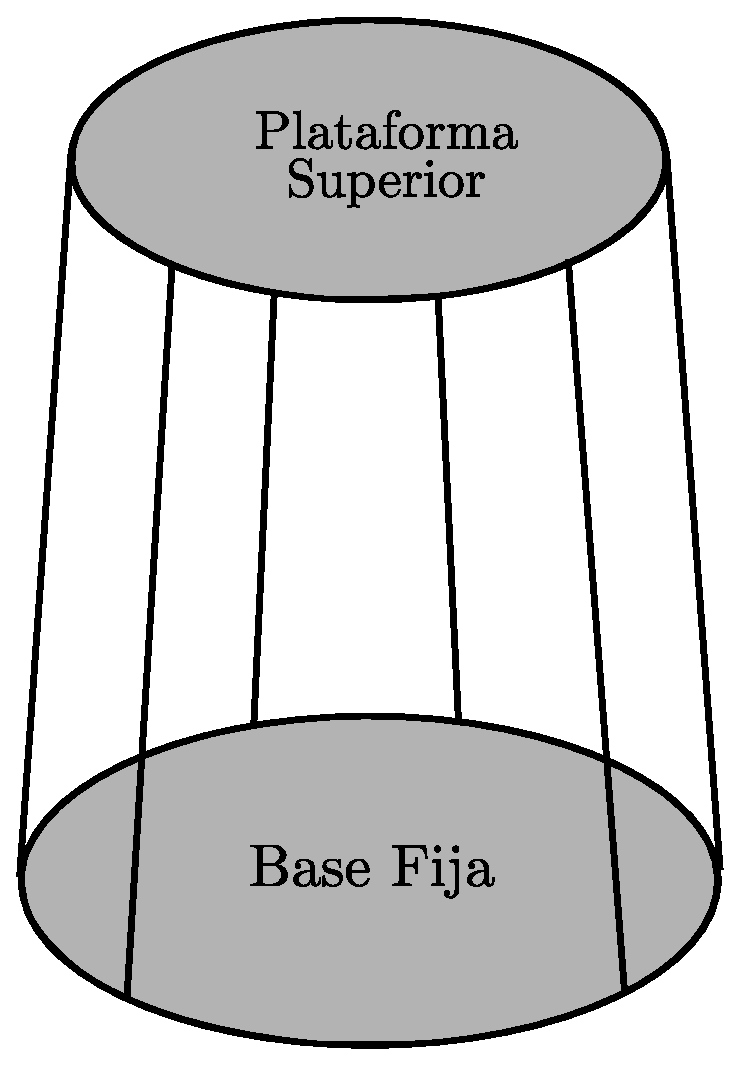
\includegraphics[width=0.5\columnwidth]{Figures/stewart1.eps}
        \caption{Esquema Plataforma Stewart}
        \label{fig:stewart1}
    \end{subfigure}
    \hfill
    \begin{subfigure}[b]{0.45\textwidth}
       \centering
        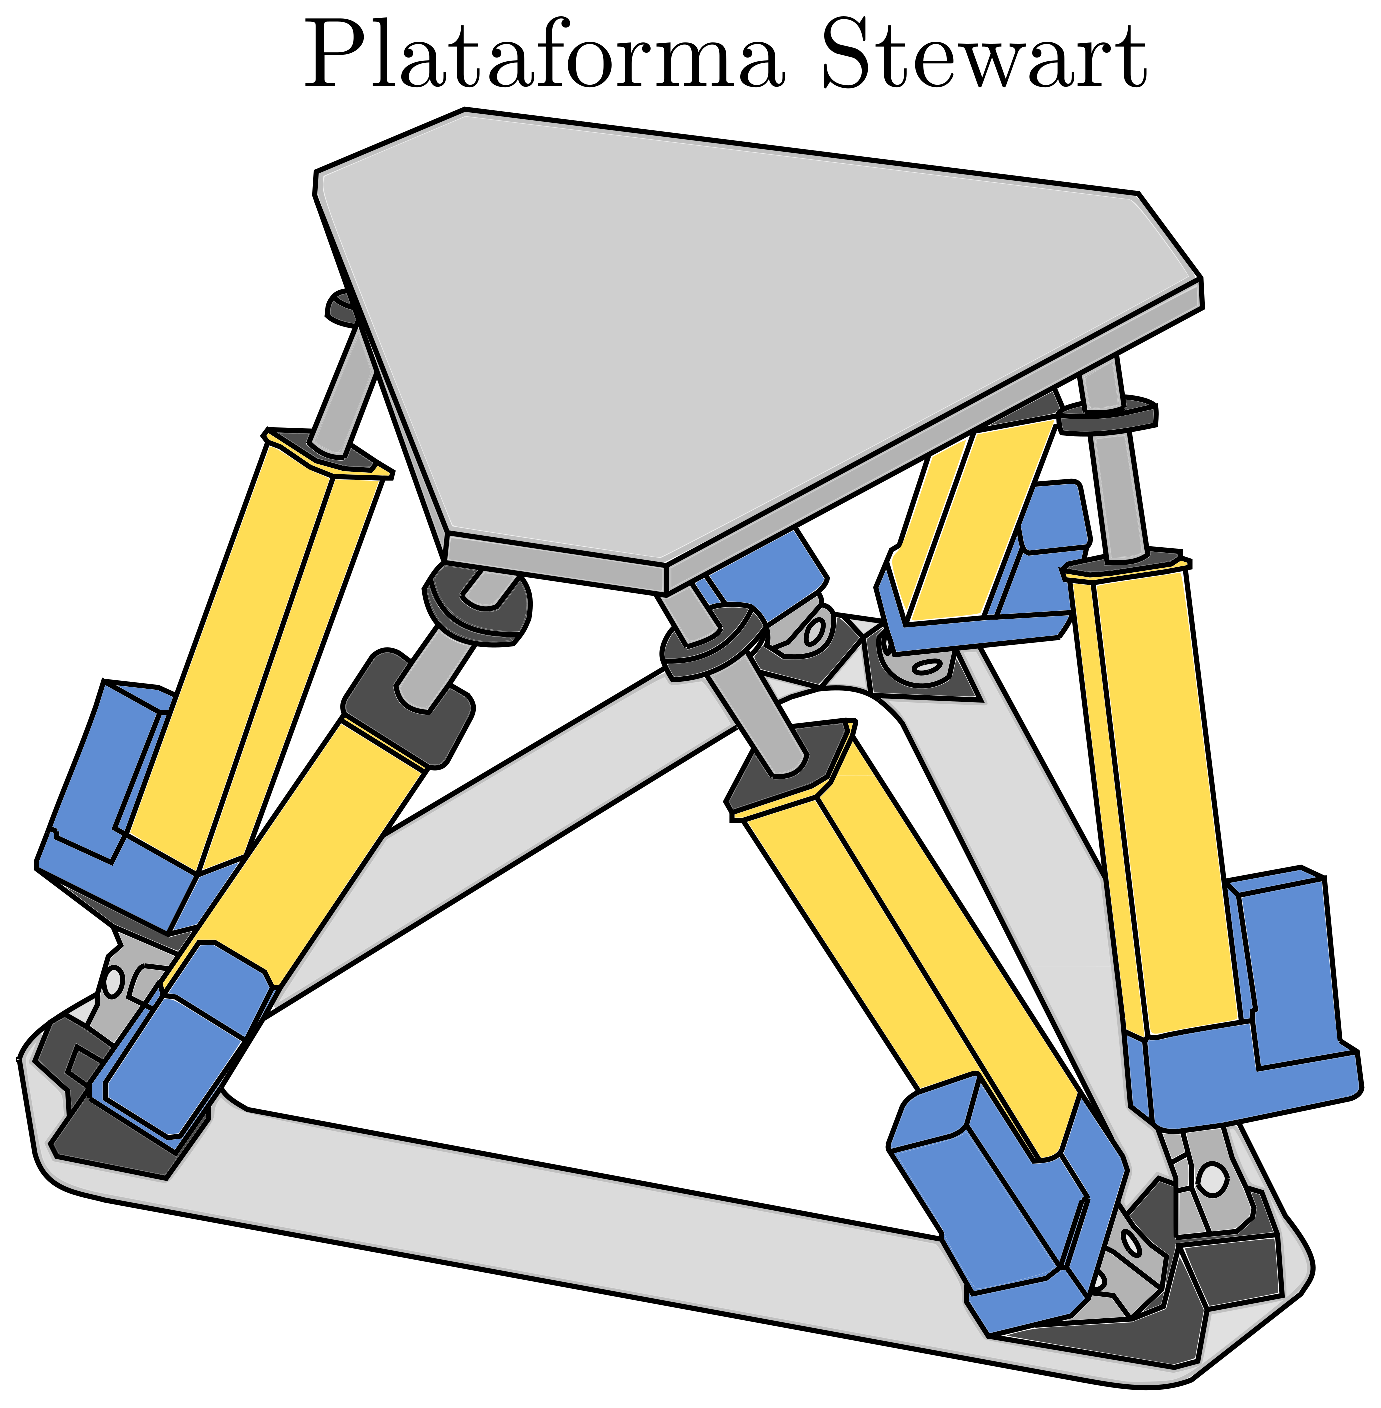
\includegraphics[width=0.7\columnwidth]{Figures/stewart3.eps}
        \caption{Plataforma Stewart}
        \label{fig:stewart2}
    \end{subfigure}
   \caption{Plataforma Stewart}
   \label{fig:StewartPlatform}
\end{figure}






\section{Estado del arte}
\lhead[\thepage]{Sección \thesection. Estado del arte}

Una plataforma Stewart es un sistema mecánico diseñado para poder manipular la posición (movimiento lateral, longitudinal y vertical) y orientación (pitch, roll \& yaw) de una plataforma sostenida en paralelo a una base de montaje fija. Dicha plataforma es manipulada a través de actuadores lineales cuyos extremos son fijados en ambas plataformas mediante junturas móviles. La configuración más común de una plataforma Stewart comprende de 6 actuadores lineales, como se aprecia en la Figura \ref{fig:StewartPlatform}, brindando así soporte y precisión al movimiento buscado.

Este tipo de manipulador paralelo de 6 DOFs se desarrolló en 1965 por \textit{Stewart} \cite{stewart1965} para simulaciones de vuelo, siendo conocida así como la plataforma Stewart. También es conocido como Gough-platform quien presentó su uso práctico del sistema \cite{stewart1965}.
\textit{Earl and Rooney} \cite{earl1983kinematicMD} analizaron la estructura cinemática para aplicaciones robóticas y sus interconexiones en serie y paralelas.  
En \cite{do1988InverseDA} usaron el método Newton-Euler para resolver la dinámica inversa de la plataforma Stewart, en ausencia de fricción en las articulaciones y brazos. 
Por otro lado, en \cite{geng1992} se desarrollaron las ecuaciones de movimiento de Lagrange relacionadas con la geometría y distribución de inercia del manipulador.

Este sistema es utilizado actualmente en diversas aplicaciones debido a la versatilidad en el movimiento que posee, tales como sistemas de posicionamiento de antenas/radares y paneles solares \cite{lin2006disturbance,keshtkar2016adaptive}, aplicaciones en la medicina \cite{boian2004dual,girone2001stewart}, simuladores de vuelo en tiempo real \cite{pradipta2013development, huang2017incremental}, plataforma ball and plate \cite{bang2018ballandplate,kassem2015ballandplatecomparison}, etc. 

Debido a la gran cantidad de grados de libertad que posee junto a su no linealidad, conlleva a ser un sistema complejo de controlar de forma eficiente. La dinámica de la plataforma suele ser simulada en distintas investigaciones con distintos software de simulación como Matlab o ADAMS \cite{tajdari2021discrete,liu2023fuzzy}, ya que brindan un mejor modelado al considerar distintas restricciones tales como colisión de objetos, rigidez y elasticidad de cuerpos rígidos, fricción entre superficies, etc. 

Muchos autores han estudiado la formulación del modelo dinámico y su simulación de forma detallada \cite{bingul2012modeling}, además de distintos diseños de control tales como control predictivo basado en modelos (MPC) \cite{nadimi2006model}, control de modo deslizante (SMC) \cite{jouini2013modeling,chalanga2015smooth}, regulador cuadrático lineal (LQR) \cite{rossell2015tracking}, control integral cuadrático lineal (LQI) \cite{tajdari2021discrete}, entre otros. Sin embargo, el control más común es el proporcional integral derivativo (PID) \cite{liu2023fuzzy,yang2008modeling,csumnu2017motor}, que en la mayoría de los casos posee una estructura descentralizada, es decir, el controlador es una matriz diagonal de controladores PID de una entrada y una salida \cite{astrom19951pidcontrollers,skogestad2005multivariable}.
Los análisis anteriores de los controladores PID se basan en la obtención de las constantes proporcional, integral y derivativa, así como se realiza en \cite{liu2023fuzzy} mediante un diseño de control difuso (Fuzzy), o como en \cite{silva2006lqr} mediante un control LQR y LQI para sistemas mecánicos generales. Todos estos diseños de control han demostrado un aumento en la efectividad y eficiencia del control de la plataforma Stewart, sin embargo son controles descentralizados \cite{albertos2006multivariable} y además para seguimiento de señales tipo escalón como referencia. Al ser controles descentralizados, es decir con estructura diagonal de controladores SISO, consideran inexistente la interacción entre los distintos actuadores, facilitando la implementación considerablemente. Sin embargo, el diseño de un controlador MIMO PID full, es decir, una matriz de controladores PID con todos sus elementos distintos de cero en general \cite{albertos2006multivariable}, si consideraría las interacciones entre los distintos actuadores pudiendo así mejorar el desempeño del control. Este tipo de control MIMO PID full no ha sido reportado en la literatura para el control de este tipo de plataformas.

Para lograr un mejor rendimiento en el control, es posible ocupar métodos numéricos de optimización para los controladores. Distintos autores han utilizado diferentes formas de optimización tales como en \cite{choubey2021optimized} utilizando un \textit{squirrel search algorithm}, en \cite{tajdari2021optimizer} mediante una red neuronal artificial o en \cite{silva2006lqr} donde se utiliza un algoritmo numérico de optimización. Estos algoritmos demuestran una mejora significativa en los tipos de control, logrando un mejor seguimiento de las señales de referencia. En el caso de un controlador MIMO PID, utilizar estos algoritmos en las versiones descentralizadas mejorarían significativamente su desempeño, optimizando los controladores comúnmente utilizados en este tipo de plataforma por la mayoría de los autores.

Por otro lado, en el ámbito de seguimiento de señales sinusoidales, se han estudiado las limitaciones del rendimiento de sistemas lineales multivariables en el seguimiento de referencias sinusoidales en \cite{su2003performance,su2005performance,su2009performance}. Se analizan distintos casos de disponibilidad de datos de la referencia al controlador, para determinar la influencia directa del acceso a la información en el rendimiento. Se demuestra que el rendimiento solo depende de la frecuencia de la referencia sinusoidal y de la interacción entre la referencia con los ceros de fase no mínima del sistema. Las expresiones obtenidas muestran la degradación del rendimiento según la información parcial disponible de la referencia sinusoidal. Sin embargo, el estudio del seguimiento de señales sinusoidales sobre esta plataforma no es un área muy explorada. En \cite{lin2003sinusoidal} se enfocan en un esquema adaptativo de cancelación de perturbaciones sinusoidales mediante algoritmos de diseño de tolerancia a fallos (\textit{fault tolerant pointing algorithms}). Este diseño es capaz de realizar un seguimiento en baja frecuencia, rechazar grandes perturbaciones monótonas a frecuencia media y aislar vibraciones pasivas de alta frecuencia.  

Debido a que la plataforma brinda una versatilidad de movimientos gracias a sus 6 grados de libertad, se da la posibilidad que las señales de cada actuador posean distintas frecuencias (asumiendo movimientos sinusoidales), es por esto que, poder garantizar un controlador que permita asignar la frecuencia que necesita cada actuador a cada componente del controlador MIMO, representaría una mejora significativa para este sistema. Con esto se lograría un rendimiento eficiente individualizado de cada actuador mediante un solo controlador MIMO, para distintos tipos de señales de referencia como escalones o sinusoidales. Este tipo de problema de seguimiento sinusoidal para distintas frecuencias no ha sido estudiado directamente en la plataforma Stewart. Para la resolución de este problema, es posible desarrollar un seguimiento a señales de referencia sinusoidales en base a un diseño de control LQR para sistemas generales según \cite{lin1996outputregulation,yan2016outputregulation,huang2004bookoutputregulation}. Basado en el principio del modelo interno, este tipo de control garantiza un seguimiento óptimo de la referencia sinusoidal en estado estacionario. Debido a esto, el enfoque de la investigación radica en la obtención de un controlador MIMO para la plataforma Stewart, tal que garantice un seguimiento eficiente en estado estacionario de señales de referencia sinusoidales de distinta frecuencia, desarrollando así un control estabilizante para cada actuador del sistema multivariable.


\section{Principales contribuciones}
\lhead[\thepage]{Sección \thesection. Principales contribuciones}

%Esta tesis tiene como objetivo diseñar un control multivariable para la plataforma Stewart, tal que posea mejor desempeño que las versiones descentralizadas del control MIMO y a sus variantes optimizadas mediante algoritmos numéricos. Además, se busca diseñar un control que garantice un seguimiento eficiente en estado estacionario de señales de tipo sinusoidales de distinta frecuencia en la referencia. \\

Las dos principales contribuciones de esta Tesis se pueden resumir de la siguiente manera:
\begin{enumerate}
    \item Se propone un diseño de controlador MIMO PID full sintetizado en base a un control LQI. El desempeño de este controlador se compara con versiones descentralizadas del mismo controlador MIMO PID, así como con versiones optimizadas de los controladores descentralizados mediante un algoritmo numérico basado en un descenso del gradiente simple. Las simulaciones son desarrolladas mediante el programa Matlab Simulink por Simscape, especialmente diseñado para este tipo de plataformas multivariables, ya que incluye complejas interacciones internas de la parte mecánica y dinámica del sistema, facilitando una simulación más real de la plataforma. Los resultados obtenidos son en base a referencias de tipo escalón y sinusoidal, logrando un análisis completo de los distintos tipos de movimientos que es posible otorgar a la plataforma Stewart. Se ha demostrado que el control es eficiente para señales de tipo escalón, pero no para señales sinusoidales.
    
    \item A base de lo anterior, se propone un nuevo tipo de control que logra garantizar un seguimiento eficiente en estado estacionario para señales de referencia de tipo sinusoidal de distintas frecuencias para sistemas lineales. Para esto, mediante el concepto de Output Regulation basado en el principio del modelo interno se obtiene el controlador buscado de la plataforma Stewart. El controlador se diseña en base a un control LQR, que estabiliza las dinámicas internas de la plataforma, permitiendo el seguimiento sinusoidal de la referencia al utilizar información de la misma en el diseño del controlador. Se ilustran simulaciones de los resultados junto a un análisis comparativo con los diseños de control anteriores.
    
\end{enumerate}


\section{Publicaciones asociadas}
\lhead[\thepage]{Sección \thesection. Publicaciones asociadas}

Los principales trabajos asociados a esta Tesis son:
\begin{itemize}
    \item \textbf{Título del artículo:} Control of a Stewart platform using a MIMO PID controller. \\
        \textbf{Autores:} Tomás E. Bernal, Marco A. Gordon, Francisco J. Vargas, Alejandro A. Pacheco. \\
        \textbf{Publicado en:} Conferencia Andescon 2024.
    \item \textbf{Título del artículo:} Step and Sinusoidal Tracking Techniques for Stewart Platforms \\ 
        \textbf{Autores:} Tomás E. Bernal, Marco A. Gordon, Francisco J. Vargas, Alejandro A. Pacheco. \\
        \textbf{Estado:} En desarrollo para Revista. 
\end{itemize}

\section{Organización de la Tesis}
\lhead[\thepage]{Sección \thesection. Organización de la tesis}

La presente Tesis se organiza mediante capítulos ordenados de la siguiente manera:
\begin{itemize}
    \item  En el Capítulo \ref{cap:Notación y preliminares} se detallan definiciones y notaciones importantes para el desarrollo de la Tesis. 
    \item El Capítulo \ref{cap:modeladoStewart} tiene por objetivo desarrollar el modelado de la plataforma Stewart, ecuaciones dinámicas y linealización del sistema.
    \item En el Capítulo \ref{cap:mimoPID} se diseña el control PID MIMO full de la plataforma. Además, se analiza el desempeño del controlador con versiones descentralizadas y optimizadas del mismo.
    \item En el Capítulo \ref{cap:OutputRegulation} se diseña un nuevo tipo de control de la plataforma Stewart que garantiza un seguimiento eficiente en estado estacionario para señales de referencia de tipo sinusoidal de distintas frecuencias. 
    \item Finalmente en el Capítulo \ref{cap:Conclusiones} se mencionan las conclusiones y posibles trabajos futuros.
\end{itemize}

	
% =========================== CAPÍTULO 2 ============================ %
\lhead[\thepage]{\thechapter. \rightmark}
\rhead[\leftmark]{\thepage}
\renewcommand{\headrulewidth}{0.5pt}
\lfoot[]{}
\cfoot[]{}
\rfoot[]{}
\renewcommand{\footrulewidth}{0pt}
	
\fancypagestyle{plain}{
	\fancyhead[L]{}
	\fancyhead[C]{}
	\fancyhead[R]{\thepage}
	\fancyfoot[L]{}
	\fancyfoot[C]{}
	\fancyfoot[R]{}
	\renewcommand{\headrulewidth}{0.5pt}
}
	\chapter{PRELIMINARES Y GENERALIDADES SOBRE CONTROL LQR/LQI}
\label{cap:Notación y preliminares}

El principal propósito de este capítulo es otorgar la introducción sobre las notaciones, definiciones y diseños de control generales utilizados en la Tesis.

\section{Notación} \label{sec:notación}
\lhead[\thepage]{Sección \thesection. Notación}

\subsection{Matrices y vectores} \label{sec:matrices}

Un vector $a\in\mathbb{R}^n$ con notación $\vec{a}$ representa explícitamente un vector con dirección y magnitud en el espacio. En caso que los vectores no representen una dirección, se omite la notación con la flecha superior. Además, para $a\in \mathbb{R}^n$ y $b\in \mathbb{R}^n$ dos vectores, se define el producto cruz entre ambos como $a \times b$. \\

Sea $A \in \mathbb{R}^{n\times n}$ una matriz cuadrada, el radio espectral se define de la forma:
\begin{equation*}
    \rho (A) = \max \{ |\lambda_1|,\ |\lambda_2|,\ \cdots ,\ |\lambda_n| \},
\end{equation*}
donde $\lambda_1, \lambda_2 , \cdots , \lambda_n$ son los autovalores de $A$. El $i$-ésimo valor singular de $A$ se denota como  $\sigma_i(A)$ y el mayor valor singular se define como $\sigma_{\max}(A)$. 

La transpuesta de la matriz $A$ se denota como $A^{\top}$. 

La traza de la matriz $A$ se define como la suma de los elementos de su diagonal principal, es decir:
\begin{equation*}
    \textrm{trace}\left\{ A \right\} = a_{1,1} + a_{2,2} + \hdots + a_{n,n},
\end{equation*}
donde $a_{n,n}$ son los elementos de la $n$-ésima fila y $n$-ésima columna de A. \\

Dada una matriz $B \in \mathbb{R}^{m \times n}$, se define el operador $vec(\cdot)$ de la matriz $B$ como la operación de vectorización (por columnas):
\begin{equation*}
    vec(B)= \left[b_{1,1},\dots ,b_{m,1},b_{1,2},\dots , b_{m,2}, \dots ,b_{1,n}, \dots , b_{m,n} \right]^{\top},
\end{equation*}
donde $b_{m,n}$ son los elementos de la $m$-ésima fila y $n$-ésima columna de la matriz $B$.\\
Sea la variable $v=vec(B) \in \mathbb{R}^{mn}$, al conocer las dimensiones originales de la matriz, es posible reconstruir la matriz $B \in \mathbb{R}^{m \times n}$ aplicando la operación inversa $vec^{-1}(\cdot)$ \cite{magnus1988matrix}. Esta operación inversa es posible calcularla como:
\begin{equation*}
    vec^{-1}(v) = \left( vec(I_n)^{\top} \otimes I_m \right) \left(I_n \otimes v \right),
\end{equation*}
donde $I_n$ e $I_m$ son las matrices identidad de dimensiones $n$ y $m$ respectivamente, y $\otimes$ denota al producto de Kronecker. \\

Sean las matrices $A \in \mathbb{R}^{m\times n}$ y $B \in \mathbb{R}^{p\times q}$, el producto de Kronecker $A \otimes B \in \mathbb{R}^{mp \times nq}$ se define como
\begin{equation*}
    A \otimes B \triangleq \begin{bmatrix} 
    a_{11}B & \cdots & a_{1n}B \\
    \vdots & \ddots & \vdots \\
    a_{m1}B & \cdots & a_{mn}B
    \end{bmatrix},
\end{equation*}
donde $a_{mn} \in \mathbb{R}$ denota el $(m,n)$ elemento de $A$. Se mencionan dos propiedades importantes acerca de el producto de Kronecker a continuación \cite{bernstein2009matrix,horn13,meyer2000matrix}:
\begin{itemize}
    \item Sean $A,B,C,D$ matrices de dimensiones apropiadas, tales que los productos $AC$ y $BD$ están bien definidos, entonces 
    \begin{equation*}
        (A \otimes B) (C \otimes D) = (AC) \otimes (BD).
    \end{equation*}
    \item Sean $A,X,B$ matrices de dimensiones apropiadas, tales que el producto $AXB$ está bien definido, entonces 
    \begin{equation*}
        vec(AXB)= (B^{\top} \otimes A ) vec(X).
    \end{equation*}
\end{itemize}

Sea $A \in \mathbb{R}^{m\times n}$ y $B \in \mathbb{R}^{m\times n}$, se define el producto de Hadamard $A\odot B \in \mathbb{R}^{m \times n}$ como
\begin{equation*}
    A \odot B \triangleq \begin{bmatrix} 
    a_{11} b_{11} & \cdots & a_{1n} b_{1n} \\
    \vdots & \ddots & \vdots \\
    a_{m1}b_{m1} & \cdots & a_{mn}b_{mn}
    \end{bmatrix},
\end{equation*}
donde $a_{mn} \in \mathbb{R}$ denota el $(m,n)$ elemento de $A$ y $b_{mn} \in \mathbb{R}$ denota el $(m,n)$ elemento de $B$ \cite{bernstein2009matrix}.


\subsection{Normas Vectoriales}

\begin{itemize}
    \item Sea $x \in \mathbb{R}^{n}$ un vector, donde el $i$-ésimo elemento de $x$ se denota como $x\{i\}$. Su norma $\norm{x}_p$, con $p \in \mathbb{N}$ se define como
    \begin{align*}
        \norm{x}_p &\triangleq \left( \sum_{i=1}^n \abs{x \{i \}}^p \right)^{1/p}
    \end{align*} 
\end{itemize}

\subsection{Señales}

\begin{itemize}
    \item Dada una señal en tiempo continuo como $x(t)$, cuando el tiempo tiende a infinito, es decir $t \to \infty$, la señal en estado estacionario se denota como $x_\infty$.
\end{itemize}

\section{Control LQR/LQI} \label{sec:lqicontrol}
\lhead[\thepage]{Sección \thesection. Control LQI}

El regulador cuadrático lineal (LQR) es una técnica de control óptimo que busca diseñar un sistema de control que minimice un costo asociado al desempeño de un sistema dinámico. Mediante una función de costo cuadrática, LQR calcula las ganancias óptimas para generar una señal de control que mantenga al sistema estable y eficiente.


\subsection{Regulador Cuadrático Lineal (LQR)}

El control LQR llamado Regulador Cuadrático Lineal, es un tipo de control encargado de regular los estados internos de un sistema dinámico, garantizando estabilidad en el control. La definición del diseño LQR se extrae del libro \textit{Control System Design} \cite{goodwin2001control}. 

Se considera un sistema lineal general definido en variables de estados como:
\begin{subequations} \label{eq:sys_general_varestados}
    \begin{align}
        \Dot{x}(t) & = A x(t) + B u(t), \\
        y(t) & = C x(t) + D u(t)
    \end{align}    
\end{subequations}

Este regulador se caracteriza por ser un control óptimo, debido a que minimiza una función de coste especifica, apreciada en la ecuación siguiente. El diseño se basa en 3 matrices de ponderación ($Q,R,S$), encargadas de la ponderación de los estados, los esfuerzos de control en la entrada y la relación de ambas en el sistema. 

\begin{equation} \label{eq:lqr_funcioncoste}
    J_{LQR} = \int_0^\infty \left( x(t)^{\top} Q x(t) + u(t)^{\top} R u(t) + 2 x(t)^{\top} S u(t)\right) dt,
\end{equation}
donde $Q=Q^{\top}\geq0$, $R=R^{\top}>0$ y $S$ son las matrices de ponderación. 

Una de las formas de resolver el problema de optimización de la función de costo es mediante programación dinámica, como se demuestra en \cite{bertsekas2012dynamic} donde se detalla el proceso de la programación dinámica para funciones de coste. La solución que optimiza que minimiza la función de coste se define como
\begin{equation}
    u^*(t)= -K_x(t) \cdot x(t)
\end{equation}
con $x(t)$ los estados del sistema lineal de \eqref{eq:sys_general_varestados} y la matriz $K_x(t)$ de realimentación de los estados definida como

\begin{equation}
    K_x(t) = R^{-1} B^{\top} P(t)
\end{equation}

donde $P(t)$ es la solución a la ecuación diferencial de Riccati de tiempo continuo
\begin{equation}
    -\dot{P}(t) = A^{\top} P(t) + P(t) A - P(t) B R^{-1} B^{\top} P(t) + Q
\end{equation}
con $A,B,C$ matrices del sistema lineal en variables de estados. 

Si el sistema $(A,B)$ es estabilizable y los estados son detectables, se tiene que para $t \to \infty$ la solución de la ecuación diferencial de Riccati converge a un estado estacionario $P_\infty$. 

\begin{mybox}{}
    \begin{lemma} \label{lem1:riccati_infinto}
        Si P(t) converge en $t \to \infty$, su valor en estado estacionario $P_\infty$ satisface la siguiente ecuación algebraica de Riccati para tiempo continuo \cite{goodwin2001control}:
        \begin{equation}
            0 = A^{\top} P_\infty + P_\infty A - P_\infty B R^{-1} B^{\top} P_\infty + Q
        \end{equation}
        Con el valor estacionario $P_\infty$ de la ecuación de Riccati en tiempo continuo, entonces es posible definir un control óptimo estable del sistema como:
        \begin{equation}
            u^*(t) = - K_{x_\infty} x(t)
        \end{equation}
         donde $K_{x_\infty} = R^{-1} B^{\top} P_\infty$
    \end{lemma}
\end{mybox}

\begin{proof}
    La demostración del Lema \ref{lem1:riccati_infinto} se encuentra en \cite{goodwin2001control}.
\end{proof}

En la Figura \ref{fig:lqr_scheme} se puede apreciar el esquema de control LQR para la planta $G$, con $u$, $x$ e $y$ la actuación, los estados y la salida de la planta respectivamente.

\begin{figure}[ht]
\centering
    
\includegraphics[width=0.4\columnwidth]{Figures/Preliminares/lqr_scheme.eps}
    \caption{Esquema de control LQR.}
    \label{fig:lqr_scheme}
\end{figure}

El requisito principal para el diseño de control LQR es tener disponibles los estados internos del sistema. El problema radica en que no siempre estos estados estarán disponibles y/o medibles en la salida del sistema. Para solucionar esto es posible utilizar un observador de Luenberger (o un filtro de Kalman si se está en presencia de ruidos gaussianos) el cual se encarga de estimar los estados del sistema \cite{skogestad2005multivariable}.

El control óptimo LQR está enfocado en la regulación de estados, no así en el seguimiento de referencia como tal. Es por esto que mediante el principio del modelo interno es posible incluir un estado extra encargado de el seguimiento de la referencia como se define en el diseño de control LQI a continuación.

\subsection{Control Integral Cuadrático Lineal (LQI)}

Mediante una acción integral es posible incluir el seguimiento de referencia en el problema de regulación manteniendo un diseño de control optimo \cite{feng2007lqi}.

Sea el sistema lineal \eqref{eq:sys_general_varestados} en variables de estados, considerando $D$ cero, la referencia $r$ a seguir del sistema y la salida medible $y$, se define el error de seguimiento como:
\begin{align}
    e(t) & = r(t) - y(t) \notag \\
    & = r(t) - C x(t)
\end{align}

Se establece un estado aumentado del sistema, en donde se incluye la integral del error como un estado extra.

\begin{equation}
    z(t) = \begin{bmatrix}
        x(t) \\ \int e(t)
    \end{bmatrix} 
    = \begin{bmatrix}
        x(t) \\ x_i(t)
    \end{bmatrix}
\end{equation}

Se describe el sistema aumentado en variables de estados de la forma:

\begin{equation}
    \begin{bmatrix}
        \dot{x}(t) \\ \dot{x}_i(t)
    \end{bmatrix} = \underbrace{\begin{bmatrix}
        A & 0 \\ -C & 0 
    \end{bmatrix}}_{A_a} \begin{bmatrix}
        x(t) \\ x_i(t)
    \end{bmatrix} + \underbrace{\begin{bmatrix}
        B \\ 0
    \end{bmatrix}}_{B_a} u(t) + \begin{bmatrix}
        0 \\ I
    \end{bmatrix} r(t)
\end{equation}
donde $I$ es la matriz identidad de dimensión apropiada. 

Dado que se busca que el sistema en estado estacionario cumpla $\dot{x}_\infty = A x_\infty + B u_\infty$ y que $\dot{x}_{i_\infty} = e_\infty  = 0$, el sistema aumentado anterior es equivalente a:

\begin{equation} \label{eq:sys_aumentado_lqi}
    \begin{bmatrix}
        \dot{x}(t) \\ \dot{x}_i(t)
    \end{bmatrix} = \underbrace{\begin{bmatrix}
        A & 0 \\ -C & 0 
    \end{bmatrix}}_{A_a} \begin{bmatrix}
        x(t) \\ x_i(t)
    \end{bmatrix} + \underbrace{\begin{bmatrix}
        B \\ 0
    \end{bmatrix}}_{B_a} u(t)
\end{equation}

Con el sistema aumentado, el diseño de control se traduce en un control LQR para el estado aumentado $z(t)=\begin{bmatrix} x(t)^{\top} & x_i(t)^{\top} \end{bmatrix}^{\top}$.

La función de coste asociada al problema de control LQI es:
\begin{equation} \label{eq:lqi_funcioncoste}
    J_{LQI} = \int_0^\infty \left( z(t)^{\top} Q z(t) + u(t)^{\top} R u(t) + 2 z(t)^{\top} S u(t)\right) dt,
\end{equation}
donde $Q=Q^{\top}\geq0$, $R=R^{\top}>0$ y $S$ son las matrices de ponderación del estado aumentado, del esfuerzo de control en la entrada, y de la relación entre ambos elementos.

La solución óptima al funcional de costo asociado es:
\begin{equation}
    u^*(t) = -K_x x(t) - K_i x_i(t)
\end{equation}
donde 
\begin{equation}
    \begin{bmatrix}
        K_x & K_i 
    \end{bmatrix} = R^{-1} B_a^{\top} P_\infty
\end{equation}
con $P_\infty$ la solución a la ecuación algebraica de Riccati en tiempo continuo dada por:
\begin{equation}
    0 = A_a^{\top} P_\infty + P_\infty A_a - P_\infty B_a R^{-1} B_a^{\top} P_\infty + Q
\end{equation}
con las matrices $A_a$ y $B_a$ del sistema aumentado \eqref{eq:sys_aumentado_lqi}.

El control LQI logra una solución estable y óptima respecto al funcional de costo asociado, además de garantizar error de seguimiento cero en estado estacionario para señales de referencias de tipo escalón \cite{young1972approach}.

En la Figura \ref{fig:lqi_scheme} se ilustra el esquema de control LQI para la referencia $r$, con $u$, $x$ e $y$ la actuación, los estados y la salida de la planta $G$ respectivamente.

\begin{figure}[ht]
\centering
    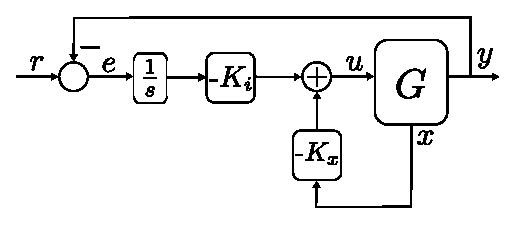
\includegraphics[width=0.6\columnwidth]{Figures/Preliminares/lqi_scheme.eps}
    \caption{Esquema de control LQI.}
    \label{fig:lqi_scheme}
\end{figure}



\newpage
\section{Output Regulation} \label{sec:outputregulation}
\lhead[\thepage]{Sección \thesection. Output Regulation}

El desarrollo conceptual y teórico del problema Output Regulation es obtenido directamente desde el libro \textit{Nonlinear Output Regulation: Theory and Applications} \cite{huang2004bookoutputregulation}.

Sea el sistema lineal general con perturbación, descrito en variables de estados de la forma:

\begin{subequations} \label{eq:sys_general_outputregulation}
    \begin{align}
        \Dot{x}(t) & = A x(t) + B u(t) + E_d d(t), \quad x(0) = x_0, \quad t \geq 0,\\
        y(t) & = C x(t) + D u(t) + F_d d(t),\\
        e(t) & = C x(t) + D u(t) + F_d d(t) - r(t)
    \end{align}    
\end{subequations}

donde $x(t)$ es el estado $n$-dimensional del sistema, $u(t)$ la entrada $m$-dimensional del sistema, $r(t)$ la referencia deseada, $e(t)$ el error de seguimiento y $d(t)$ la perturbación.

La referencia y la perturbación se suponen que son generadas por ecuaciones diferenciales autónomas lineales, con $r_0$ y $d_0$ estados iniciales arbitrarios:
\begin{equation}
    \dot{r}(t) = A_{1r} r(t), \quad r(0)=r_0, \qquad \dot{d}(t) = A_{1d} d(t), \quad d(0)=d_0
\end{equation}

Así, se definen las señales exógenas compuestas por la referencia y la perturbación del sistema como un exosistema:
\begin{equation}
    \dot{v}(t) = A_1 v(t), \quad v(0) = v_0, \quad t \geq 0 
\end{equation}
donde
\begin{equation*}
    v(t) =\begin{bmatrix} r(t) \\ d(t) \end{bmatrix}, \quad A_1 = \begin{bmatrix} A_{1r} & 0 \\ 0 & A_{1d} \end{bmatrix}, \quad v_0 \overset{def}{=} \begin{bmatrix} r_0 \\ d_0 \end{bmatrix}
\end{equation*}

Con esto, se reescribe por conveniencia el sistema lineal \eqref{eq:sys_general_outputregulation} en un sistema lineal compuesto dado por:
\begin{subequations} \label{eq:sys_compuesto_outputregulation}
    \begin{align}
        \Dot{x}(t) & = A x(t) + B u(t) + E v(t),\\
        \dot{v}(t) & = A_1 v(t), \\ 
        e(t) & = C x(t) + D u(t) + F v(t)
    \end{align}    
\end{subequations}

con $v(t)$ la señal exógena $q$-dimensional, $\begin{bmatrix} E \\ F \end{bmatrix} = \begin{bmatrix} 0 & E_d \\ -I & F_d \end{bmatrix}$, e $I$ la matriz identidad.

Sea la ley de control caracterizada por la realimentación de estados del sistema:

\begin{equation} \label{eq:lawcontrol_outputregulation}
    u(t) = K_x x(t) + K_v v(t),
\end{equation}
donde las matrices $K_x \in \mathcal{R}^{m\times n}$ y $K_v \in \mathcal{R}^{m\times q}$ son ganancias constantes.

Considerando el sistema lineal compuesto \eqref{eq:sys_compuesto_outputregulation} (que incluye a la planta y al exosistema mencionados anteriormente), junto a la ley de control \eqref{eq:lawcontrol_outputregulation}, podemos describir el sistema en lazo cerrado como:
\begin{subequations} \label{eq:sys_acl_outputregulation}
    \begin{align}
        \dot{x}_c (t) & = A_c x_c(t) + B_c v(t), \qquad x_c(0) = x_{c0}, \\
        \dot{v}(t) & = A_1 v(t), \\
        e(t) & = C_c x_c(t) + D_c v(t)
    \end{align}
\end{subequations}

donde las matrices de lazo cerrado son:
\begin{align}
    A_c & = A + B K_x, \qquad B_c = E + B K_v, \notag \\
    C_c & = C + D K_x, \qquad D_c = F + D K_v 
\end{align}

Se introduce la siguiente definición para describir los requerimientos de Output Regulation.
\begin{mybox}{}
    \begin{definition} \label{def1:acl_outputregulation}
        El sistema en lazo cerrado \eqref{eq:sys_acl_outputregulation} se dice exponencialmente estable si cumple las siguientes propiedades:
        \begin{enumerate}[leftmargin=*, labelindent=1em, label=\textbf{Propiedad \thedefinition.\arabic*}]
            \item \label{def_prop1.1} La matriz $A_c$ es Hurwitz, es decir, todos los autovalores de $A_c$ tienen parte real negativa (son estables). Además la matriz $A_1$ no posee partes reales negativas.
            \item \label{def_prop1.2} Para cualquier valor inicial de $x_{c0}$ y $v_0$ la trayectoria del sistema compuesto \eqref{eq:sys_compuesto_outputregulation} satisface:
            \begin{equation}
                \lim_{t\to \infty} e(t) = \lim_{t \to \infty} (C_c x_c(t)+D_c v(t)) = 0
            \end{equation}
        \end{enumerate}
        La ley de control del sistema en lazo cerrado debe satisfacer ambas propiedades descritas para resolver el problema lineal de Output Regulation.
    \end{definition}
\end{mybox}

\begin{assumption}
\label{assum1:regulation_assumption}
    Bajo la definición \ref{def1:acl_outputregulation} anterior, se asumen 3 condiciones para resolver el problema lineal de Output Regulation:
    \begin{enumerate}[leftmargin=*, labelindent=1em, label=\textbf{(\theassumption.\alph*)}]
        \item \label{assum1.1} $A_1$ no posee autovalores con parte real negativa. 
        \item \label{assum1.2} El par $(A,B)$ es estabilizable. 
        \item El par $\left( \begin{bmatrix} C & F \end{bmatrix}, \begin{bmatrix} A & E \\ 0 & A_1 \end{bmatrix} \right)$ es detectable.
    \end{enumerate}
\end{assumption}

\begin{mybox}{}
    \begin{lemma} \label{lem2:regulation_equation}
        Bajo la suposición \ref{assum1.1} y considerando la ley de control \eqref{eq:lawcontrol_outputregulation}, se asume que el sistema en lazo cerrado \eqref{eq:sys_acl_outputregulation} posee la \ref{def_prop1.1}. Entonces, las siguientes declaraciones son equivalentes:
        \begin{enumerate}
            \item El sistema en lazo cerrado posee la \ref{def_prop1.2}. 
            \item El controlador resuelve el problema lineal Output Regulation.
            \item Existe una única matriz $X_c$ que satisface las siguientes ecuaciones matriciales:
            \begin{align} \label{eq:lem2_eqRegulation}
                X_c A_1 = A_c X_c + B_c \notag \\
                0 = C_c X_c + D_c
            \end{align}
        \end{enumerate}
        \begin{remark}
            Resolución del sistema de ecuaciones \ref{eq:lem2_eqRegulation} demostrado en Apéndice \ref{appen1}.
        \end{remark}
    \end{lemma}
\end{mybox}

Bajo la siguiente transformación lineal es posible obtener un mejor enfoque de resolución del problema Output Regulation:
\begin{equation}
    \begin{bmatrix}
        X \\ U
    \end{bmatrix} = \begin{bmatrix}
        I_n & 0_{n\times m} \\ K_x & I_m
    \end{bmatrix} 
    \begin{bmatrix}
        X_c \\ K_v    
    \end{bmatrix}
\end{equation}

\begin{mybox}{}
    \begin{theorem} \label{teo1:OutputRegulation}
        Bajo las suposiciones \ref{assum1.1} y \ref{assum1.2}, se establece la ganancia de realimentación de control $K_x$ tal que $(A+BK_x)$ es exponencialmente estable. Luego, el problema lineal Output Regulation se puede resolver por la ley de control de realimentación de estados:
        \begin{equation}
            u(t) = K_x x(t) + K_v v(t)
        \end{equation}
        si y solo si existen 2 matrices $X$ y $U$ tales que satisfagan las ecuaciones matriciales de regulación:
        \begin{align}\label{eq:teo1_eqRegulation}
            X A_1 = A X + B U + E \notag \\
            0 = C X + D U + F
        \end{align}
                
        con la ganancia de realimentación $K_v$ dada por la transformación lineal:
        \begin{equation}
            K_v = U - K_x X
        \end{equation}
        donde las matrices $A,B,C,D,E,F$ y $A_1$ están determinadas por la planta y la referencia a seguir. 
        \begin{remark}    
         Resolución del sistema de ecuaciones \eqref{eq:teo1_eqRegulation} demostrado en Apéndice \ref{appen1}.
         \end{remark}
    \end{theorem}
\end{mybox}

En la Figura \ref{fig:output_regulation_scheme} se ilustra el esquema de control LQR Output Regulation, donde $v$ es la referencia, y $u$, $x$ e $y$ son la actuación, los estados y la salida de la planta $G$ respectivamente.

\begin{figure}[ht]
\centering
    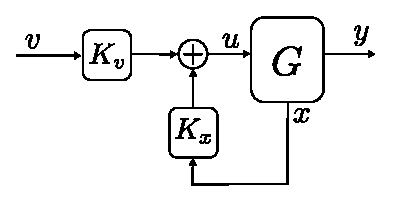
\includegraphics[width=0.45\columnwidth]{Figures/Preliminares/output_regulation_scheme.eps}
    \caption{Esquema de control LQR Output Regulation.}
    \label{fig:output_regulation_scheme}
\end{figure}


% =========================== CAPÍTULO 3 ============================ %
\lhead[\thepage]{\thechapter. \rightmark} 
\rhead[\leftmark]{\thepage}
\renewcommand{\headrulewidth}{0.5pt}
\lfoot[]{}
\cfoot[]{}
\rfoot[]{}
\renewcommand{\footrulewidth}{0pt}
	
\fancypagestyle{plain}{
	\fancyhead[L]{}
	\fancyhead[C]{}
	\fancyhead[R]{\thepage}
	\fancyfoot[L]{}
	\fancyfoot[C]{}
	\fancyfoot[R]{}
	\renewcommand{\headrulewidth}{0.5pt}
}
	\chapter{MODELADO DEL SISTEMA NO LINEAL Y LINEAL DE LA PLATAFORMA STEWART}
\label{cap:modeladoStewart}
\markboth{CAPÍTULO \thechapter. MODELADO PLATAFORMA STEWART}{CAPÍTULO \thechapter. MODELADO PLATAFORMA STEWART}

El presente capítulo tiene como principal objetivo describir el modelo no lineal de la plataforma Stewart, con sus dinámicas internas y bloques necesarios para el futuro control de la misma. Además, se desarrolla la linealización de la plataforma, factor primordial para el diseño de control en los capítulos siguientes.


%##############################################################
%##############################################################
\section{Modelo no lineal de la plataforma Stewart}
\lhead[\thepage]{Sección \thesection. Modelo No Lineal}

El modelado de una plataforma Stewart se comprende principalmente por un conjunto de bloques encargados de facilitar el manejo y control de la plataforma. Se puede observar en la Figura \ref{fig:stewart_scheme} los bloques principales del modelado de la plataforma Stewart.

\begin{figure}[ht]
\centering
    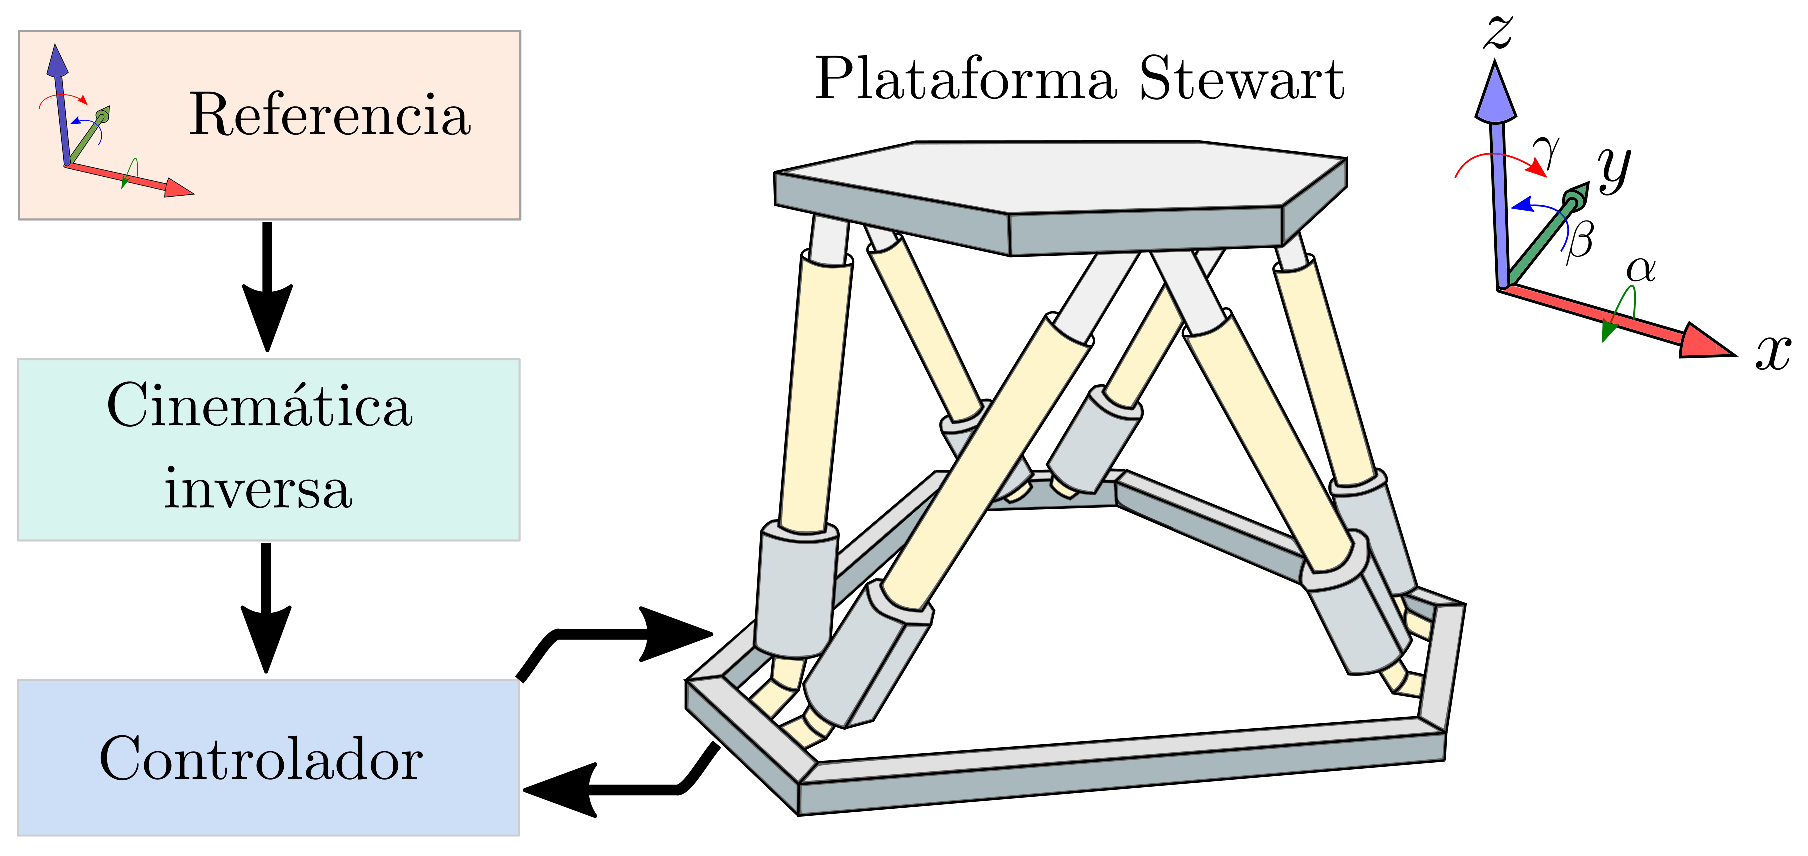
\includegraphics[width=0.6\columnwidth]{Figures/stewart_scheme.eps}
    \caption{Esquema de una plataforma Stewart.}
    \label{fig:stewart_scheme}
\end{figure}



\subsection{Bloque Referencia}

El primer bloque corresponde a la referencia global que se desea de la plataforma Stewart, es decir, describir el movimiento del centro de masa de la plataforma superior. Este movimiento describe el desplazamiento del centro de masa en los ejes $x$, $y$, $z$ representados por $P_x$, $P_y$, $P_z$, así como los movimientos de rotación de estos mismos ejes denotados como $\alpha, \beta, \gamma$.

\begin{equation} \label{eq:ref}
    q_{ref} = \begin{bmatrix}
        P_x & P_y & P_z & \alpha & \beta & \gamma
    \end{bmatrix}^{\top}
\end{equation}


\subsection{Bloque Cinemática Inversa}

El bloque de Cinemática Inversa es uno de los más importantes, ya que es el encargado de transformar el movimiento deseado del centro de masa de la plataforma superior ($q_{ref}$), al desplazamiento lineal deseado por cada brazo actuador. El análisis completo de este bloque se basa en el trabajo de \textit{Zafer Bingul y Oguzhan Karahan} en \cite{bingul2012modeling}.

\subsubsection{Largo de Brazos}

Se ilustran los puntos de conexión de los brazos entre ambas plataformas (base $B$ y superior $T$) en la Figura \ref{fig:stewart_ejes}, además de sus respectivos ejes de coordenada. Los puntos $B_i$ corresponden a las conexiones en la base, mientras que los puntos $T_i$ corresponden a los de la plataforma superior, con $i = 1,...,6 \in \mathbb{N} $.

\begin{figure}[ht]
\centering
    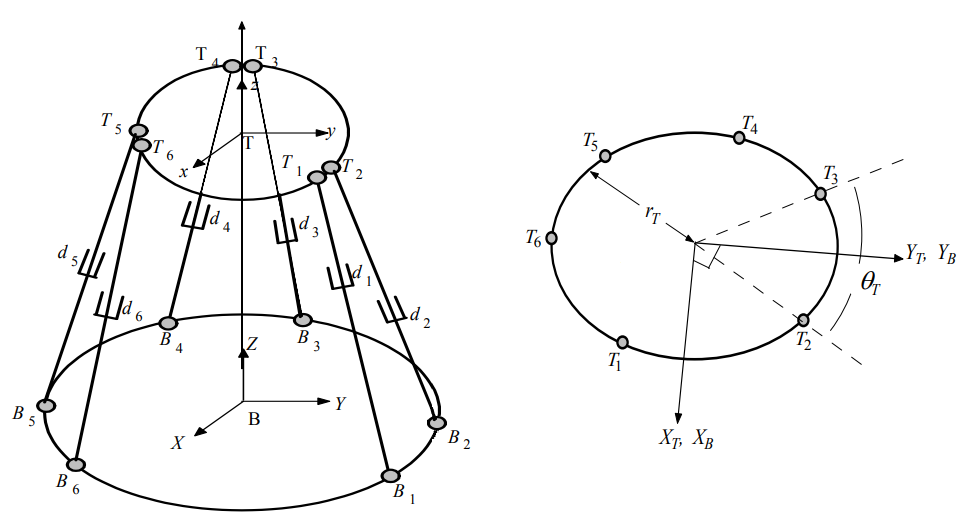
\includegraphics[width=0.8\columnwidth]{Figures/stewart_ejes.png}
    \caption{Diagrama esquemático de la plataforma Stewart (Imagen obtenida de [20]).}
    \label{fig:stewart_ejes}
\end{figure}

También desde la Figura \ref{fig:stewart_ejes} se definen los ángulos de separación entre los puntos de fijación de cada plataforma, es decir, $\theta_{T}$ para los ángulos de la plataforma superior y $\theta_{B}$ para la base. Además se define el radio de cada plataforma como $r_{T}$ y $r_{B}$ para la plataforma superior y de la base respectivamente.

Con los parámetros definidos anteriormente, se procede a modelar cada punto de conexión de la plataforma superior y de la base a sus respectivos ejes de coordenadas, mediante sus coordenadas polares de la forma:

\begin{equation}
    T_i = \begin{bmatrix} 
            T_{xi} \\ T_{yi} \\ T_{zi} 
        \end{bmatrix} = 
        \begin{bmatrix}
            r_{T} \cdot cos(\lambda_i) \\ r_{T} \cdot sin(\lambda_i) \\ 0 
        \end{bmatrix} , \quad \textrm{con} \quad
        \begin{array}{lcc}
            \lambda_i = \frac{i\pi}{3} - \frac{\theta_{T}}{2} & \textrm{para} & i=1,3,5\\
            \lambda_i = \lambda_{i-1}+\theta_{T} & \textrm{para} & i=2,4,6
        \end{array}
\end{equation}

\begin{equation}
    B_i = \begin{bmatrix} 
        B_{xi} \\ B_{yi} \\ B_{zi} 
    \end{bmatrix} = 
    \begin{bmatrix} 
        r_{B} \cdot cos(\upsilon_i) \\ r_{B} \cdot sin(\upsilon_i) \\ 0 
    \end{bmatrix} , \quad \textrm{con} \quad
    \begin{array}{lcc}
         \upsilon_i = \frac{i\pi}{3} - \frac{\theta_{B}}{2} & \textrm{para} & i=1,3,5 \\
         \upsilon_i = \upsilon_{i-1}+\theta_{B} & \textrm{para} & i=2,4,6
    \end{array}
\end{equation}

Una vez definido los puntos de conexión de ambas plataformas, se debe describir una matriz de rotación $R_{T}^{B}$ definida por los ángulos de rotación del centro de masa superior ($\alpha, \beta, \gamma$), encargada de convertir la rotación de la plataforma superior a el eje de la base. 

\begin{equation}
    R_T^B(\alpha,\beta,\gamma) = \begin{bmatrix}
        c_\beta c_\gamma & c_\gamma s_\alpha s_\beta - c_\alpha s_\gamma & s_\alpha s_\gamma + c_\alpha c_\gamma s_\beta \\
        c_\beta c_\gamma & c_\alpha c_\gamma + s_\alpha s_\beta s_\gamma & c_\alpha s_\beta s_\gamma - c_\gamma s_\alpha \\
        -s_\beta & c_\beta s_\alpha & c_\alpha c_\beta \\
    \end{bmatrix}
\end{equation}

donde $c_\alpha$, $c_\beta$ y $c_\gamma$ son abreviaciones para $cos(\alpha)$, $cos(\beta)$ y $cos(\gamma)$ respectivamente. Similarmente $s_\alpha$, $s_\beta$ y $s_\gamma$ denotan el seno de los ángulos de rotación $\alpha$, $\beta$ y $\gamma$.\\

Por otro lado, el vector $P$ de traslación del origen de la plataforma superior con respecto a la base, se define con los primeros términos de la referencia $q_{ref}$ (\ref{eq:ref}) que describen el desplazamiento lineal del eje superior.

\begin{equation}
    P = \begin{bmatrix}
        P_x & P_y & P_z
    \end{bmatrix}^{\top}
\end{equation}

De esta forma, mediante los puntos de conexión de la plataforma superior $T_i$ y de la base $B_i$, con la matriz de rotación $R_T^B$ y el vector $P$ de traslación del origen de la plataforma superior, se define el vector $L_i$ que describe el movimiento de cada brazo actuador en forma vectorial:

\begin{equation}
    L_i = R_T^B T_i + P - B_i
\end{equation}

El largo respectivo de cada brazo se define entonces como:

\begin{equation}
    l_i = \norm{L_i}_2 \quad \textrm{para} \quad i=1,...,6
\end{equation}



\subsubsection{Velocidad de Brazos (Matriz Jacobiana)}

La matriz Jacobiana es la encargada de relacionar las velocidades de cada brazo actuador a la velocidad de movimiento de la plataforma superior. Para los manipuladores paralelos se suele usar la matriz Jacobiana como:

\begin{equation}
    \dot{L} = \mathcal{J} \dot{X}
\end{equation}
donde $\dot{L}$ y $\dot{X}$ corresponden a la velocidad de los brazos y de la plataforma superior respectivamente, y $\mathcal{J}$ representa a la matriz Jacobiana.

Esta matriz Jacobiana se puede separar en 2 matrices distintas, de la forma:

\begin{equation}
    \mathcal{J} = \mathcal{J}_1 \mathcal{J}_2
\end{equation}

Para la obtención de estas matrices mencionadas, se debe analizar la vista esquemática de los brazos de la plataforma Stewart, mostrada en la Figura \ref{fig:leg_scheme}. 

\begin{figure}[ht]
\centering
    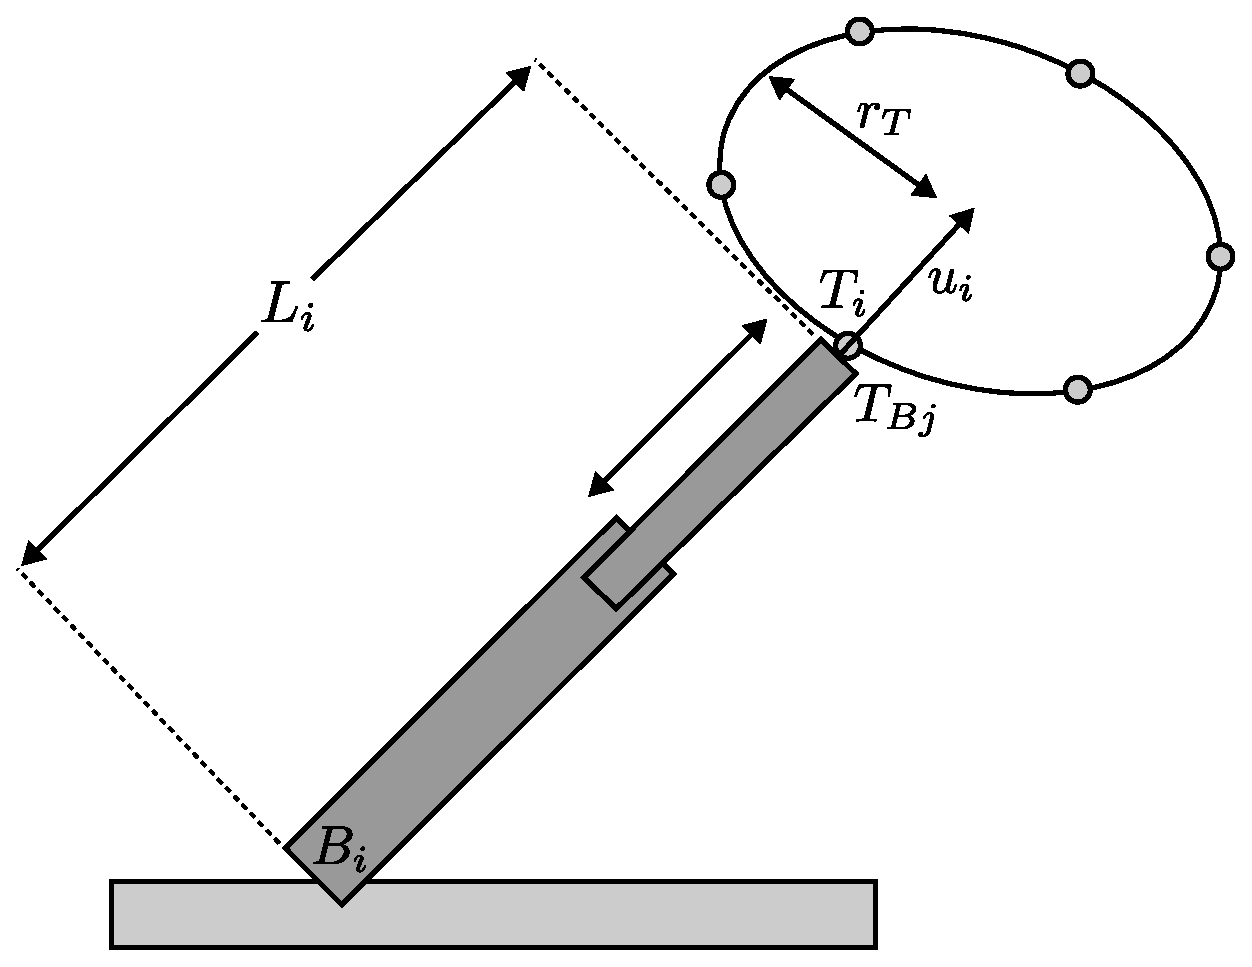
\includegraphics[width=0.5\columnwidth]{Figures/leg_scheme.eps}
    \caption{Vista esquemática de los brazos de la plataforma Stewart (Imagen obtenida de [20]).}
    \label{fig:leg_scheme}
\end{figure}

Dados los puntos de conexión $T_i$ de la plataforma superior respecto a su propio eje, de la Figura \ref{fig:leg_scheme} es posible definir $T_{Bj}$ como los puntos de conexión de la plataforma superior con referencia al sistema de coordenadas de la base dado por:
\begin{equation} \label{UpJoint_base}
    T_{Bj} = \begin{bmatrix}
        P_x & P_y & P_z
    \end{bmatrix}^{\top} + R_T^B T_i = P + R_T^B T_i
\end{equation}
donde $P$ el vector de traslación del origen de la plataforma superior respecto a la base y $R_T^B$ la matriz de rotación, definidos anteriormente.

Además, se define $\vec{u}_i$ como el vector unitario a lo largo del eje de la junta prismática de la conexión superior, de la forma:
\begin{equation}
    \vec{u}_i = \frac{B_i T_{Bj}}{\abs{L_i}} = \frac{L_i}{l_i} , \begin{cases}
        j = \frac{i+1}{2} & \textrm{si } i \textrm{ es impar}\\
        j = \frac{i}{2} & \textrm{si } i \textrm{ es par}
    \end{cases}
\end{equation}

Una vez definido los parámetros anteriores, es posible obtener la velocidad de los puntos de conexión $T_{Bj}$ derivando la ecuación \ref{UpJoint_base} con respecto al tiempo, obteniendo: 
\begin{equation}
    \vec{V}_{T_{Bj}} = \dot{T}_{Bj} = \begin{bmatrix}
        \dot{P}_x & \dot{P}_y & \dot{P}_z
    \end{bmatrix}^{\top} 
    + w \times R_T^B T_i = \dot{P} + w \times R_T^B T_i
\end{equation}
donde $w=(w_x, w_y, w_Z)$ es la velocidad angular de la plataforma superior con referencia a la base. 

\begin{equation}
    w = \begin{bmatrix}
        w_x \\ w_y \\ w_z
    \end{bmatrix}
    = \begin{bmatrix}
        cos(\beta) & 0 & 0 \\
        0 & 1 & -sin(\alpha)\\
        -sin(\beta) & 0 & cos(\alpha)
    \end{bmatrix}
    = \begin{bmatrix}
        \dot{\alpha} \\ \dot{\beta} \\ \dot{\gamma}
    \end{bmatrix}
\end{equation} 

Dado que, la proyección del vector velocidad $\vec{V}_{T_{Bj}}$ (ó $\dot{T}_{Bj}$) sobre el eje de la proyección prismática $\vec{u}_i$ de las conexiones produce la tasa de extensión de la conexión $i$, entonces es posible definir la velocidad activa $\dot{L}_i$ de los brazos actuadores como:
\begin{equation} \label{eq:leg_velocity1}
    \dot{L}_i = \vec{V}_{Bj} \vec{u}_i =  \begin{bmatrix}
        \dot{P}_x & \dot{P}_y & \dot{P}_z
    \end{bmatrix}^{\top} \cdot \vec{u}_i
    + w \times \left(R_T^B T_i \right) \cdot \vec{u}_i = \dot{P} \cdot \vec{u}_i + w \times \left(R_T^B T_i\right) \cdot \vec{u}_i
\end{equation}

Reescribiendo la ecuación \ref{eq:leg_velocity1} de forma matricial se obtiene:
\begin{equation}
    \dot{L}_i = \mathcal{J} \begin{bmatrix}
        \dot{P} \\ w
    \end{bmatrix} =
    \mathcal{J} \cdot \dot{q}_{ref} = \mathcal{J}_1 \mathcal{J}_2 \cdot \dot{q}_{ref}
\end{equation}

donde $\dot{q}_{ref}$ es la derivada del desplazamiento y orientación deseada de la plataforma superior, con las matrices Jacobianas $\mathcal{J}_1$ y $\mathcal{J}_2$ descritas como:
\begin{equation}
    \mathcal{J}_1 = \begin{bmatrix}
        u_{x1} & u_{y1} & u_{z1} & \left( R_T^B T_1 P \vec{u}_1 \right)^{\top} \\
        \vdots & \vdots & \vdots & \vdots \\
        u_{x6} & u_{y6} & u_{z6} & \left( R_T^B T_6 P \vec{u}_6 \right)^{\top} 
    \end{bmatrix}_{6\times6}
\end{equation}

\begin{equation}
    \mathcal{J}_2 = \begin{bmatrix}
        1 & 0 & 0 & 0 & 0 & 0 \\
        0 & 1 & 0 & 0 & 0 & 0 \\
        0 & 0 & 1 & 0 & 0 & 0 \\
        0 & 0 & 0 & cos(\beta) & 0 & 0\\
        0 & 0 & 0 & 0 & 1 & -sin(\alpha)\\
        0 & 0 & 0 & -sin(\beta) & 0 & cos(\alpha)
    \end{bmatrix}
\end{equation}


\subsection{Modelo Dinámico}

El análisis de las ecuaciones del modelo dinámico de la plataforma Stewart no es algo sencillo debido a la existencia de muchas cinemáticas relacionadas con la estructura de los brazos y de las plataformas, que a la vez, al estar todo conectado entre si, el efecto que se produce entre ellas es significativo. Se han descrito diversos tipos de métodos para describir la dinámica de la plataforma Stewart, pero no hay un consenso sobre cual es el más efectivo. 

En \cite{bingul2012modeling} se desarrolla el análisis a través de las energías cinéticas y potenciales de la plataforma superior y de los 6 brazos actuadores, que en conjunto, logran describir de forma general la energía cinética y potencial de la plataforma Stewart.\\

El comportamiento del sistema se basa en las ecuaciones de Euler-Lagrange aplicadas a la plataforma Stewart. A través del movimiento generalizado ($q$) de la plataforma superior y de las fuerzas generalizadas ($\tau$) aplicadas, junto a la energía cinética $E_K(q,\dot{q})$ y potencial $E_P(q)$ general de la plataforma Stewart, se define la ecuación dinámica del sistema como:
\begin{equation} \label{eq:dinamic1}
    \frac{d}{dt} \frac{dL}{d \dot{q}} - \frac{\partial L}{\partial q} = \frac{d}{dt} \left( \frac{\partial E_K(q,\dot{q})}{\partial \dot{q}} \right) - \frac{\partial E_K(q,\dot{q})}{\partial q} + \frac{\partial E_P(q)}{\partial q} = \tau
\end{equation}

Reemplazando las variables generales anteriores $q$ y $\tau$ por el movimiento deseado de la plataforma superior $q_{ref}$ y las fuerzas reales aplicadas por los actuadores, se deriva de \ref{eq:dinamic1} la ecuación dinámica como:

\begin{equation} \label{eq:dinamic2}
    M(q_{ref}) \Ddot{q}_{ref} + H(q_{ref},\dot{q}_{ref}) \dot{q}_{ref} + G(q_{ref}) = \mathcal{J}(q_{ref})^{\top} F
\end{equation}

donde $M(q_{ref})$ es la matriz de inercia, $H(q_{ref},\dot{q}_{ref})$ es la matriz Coriolis-Centrifugal y $G(q_{ref})$ es la matriz de gravedad de la plataforma móvil y brazos. Además, $\mathcal{J}(q_{ref})$ es la matriz Jacobiana y $F=\begin{bmatrix} f_1 & f_2 & f_3 & f_4 & f_5 & f_6 \end{bmatrix}^T$ con $f_i$ la fuerza aplicada por el actuador del brazo $i$ en la dirección de proyección $\vec{u}_i$ de las conexiones entre los brazos y la plataforma superior.


\subsection{Simulación Modelo No Lineal}

Se utiliza un modelo mecánico desarrollado por \textit{MathWorks} en \textit{Simscape Multibody} para el programa \textit{Matlab/Simulink}, el cual se conforma de una serie de bloques conectados entre si, representando los elementos físicos de la plataforma.

Este tipo de modelo mecánico es utilizado ampliamente ya que posee integradas las ecuaciones dinámicas del sistema, además de no linealidades, interacciones y otro tipo de fenómenos entre componentes que en los modelos matemáticos simples no están presentes. De esta forma se garantiza así un modelo más confiable y realista. Otro beneficio de este modelo mecánico es que proporciona una vista recreativa de la maquina en 3D, mostrando los movimientos y comportamientos visuales de la plataforma Stewart de forma cinematográfica. 

En la Figura \ref{fig:sim_slk_general} es posible apreciar el modelo mecánico utilizado en \textit{Matlab/Simulink}, además de sus bloques internos que lo componen y la ventana cinematográfica 3D para observar los movimientos de la plataforma.

%%%%%%%%%%%%%%% FIGURA MODELO NO LINEAL %%%%%%%%%%%%%%%%%%%%%

%##############################################################
%##############################################################

\section{Linealización de modelo no lineal de la plataforma Stewart}
\lhead[\thepage]{Sección \thesection. Linealización de modelo}
\label{sec:linealizacion_stewart}

Debido a la no linealidad del sistema, su comportamiento con respecto a una variable dada es muy impredecible, por ende, para poder diseñar un control confiable se necesita de una aproximación lineal del sistema. Para esto, se estudia la estabilidad del sistema en torno a un punto de operación. 

\subsection{Punto de Operación}

Para la obtención del punto de operación del sistema se utilizan los mismos bloques mencionados anteriormente, más específicamente los mostrados en las Figuras \ref{fig:sim_slk_general1} y \ref{fig:sim_slk_general3}. 

Se edita el bloque que describe el comportamiento de los brazos actuadores, de tal forma que la entrada sea el largo de cada brazo y que la salida sea el torque necesitado por cada actuador para mantener tal posición. En la Figura \ref{fig:sim_slk_eq} se aprecia el bloque general modificado del modelo mecánico (Figura \ref{fig:sim_slk_eq_general}) y el bloque interno modificado de cada brazo actuador con su configuración correspondiente (Figura \ref{fig:sim_slk_eq_legconfig}).

%%%%%%%%%%%%%%% FIGURA PUNTO DE OPERACION %%%%%%%%%%%%%%%%%%%%%

Se toma como punto de operación, la posición de \textit{reposo} de la plataforma en la cual los brazos no poseen extensión alguna, es decir para un largo de $0(cm)$, y la fuerza necesaria para mantener tal posición. De esta forma se describe el punto de operación definido como $(l_{EQ},\tau_{EQ})$: 

\begin{equation}
    l_{EQ} = \begin{bmatrix} 0 \\ \vdots \\ 0 \end{bmatrix}_{6\times1} \hspace{0.5cm} \Longrightarrow \hspace{0.5cm} \tau_{EQ} = \begin{bmatrix} 36.987 \\ \vdots \\ 36.987\end{bmatrix}_{6\times1}
\end{equation}

%%%%%%%%%%%%%%% FIGURA MODELO NO LINEAL %%%%%%%%%%%%%%%%%%%%%
\begin{figure}[H]
    \centering
    \begin{subfigure}[b]{0.4\textwidth}
        \centering
        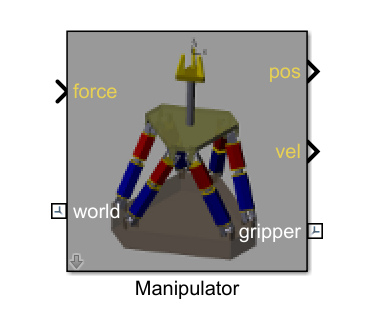
\includegraphics[width=1\columnwidth]{Figures/stewart_simulink1.png}
        \caption{Bloque general del modelo mecánico.}
        \label{fig:sim_slk_general1}
    \end{subfigure}
    \hfill
    \begin{subfigure}[b]{0.4\textwidth}
       \centering
        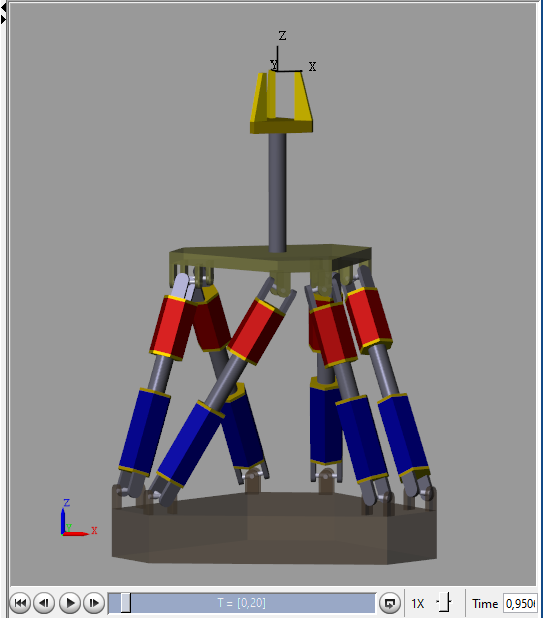
\includegraphics[width=0.75\columnwidth]{Figures/stewart_simulink3.png}
        \caption{Ventana cinematográfica 3D.}
        \label{fig:sim_slk_general2}
    \end{subfigure}
    \hfill
    \begin{subfigure}[b]{\textwidth}
       \centering
        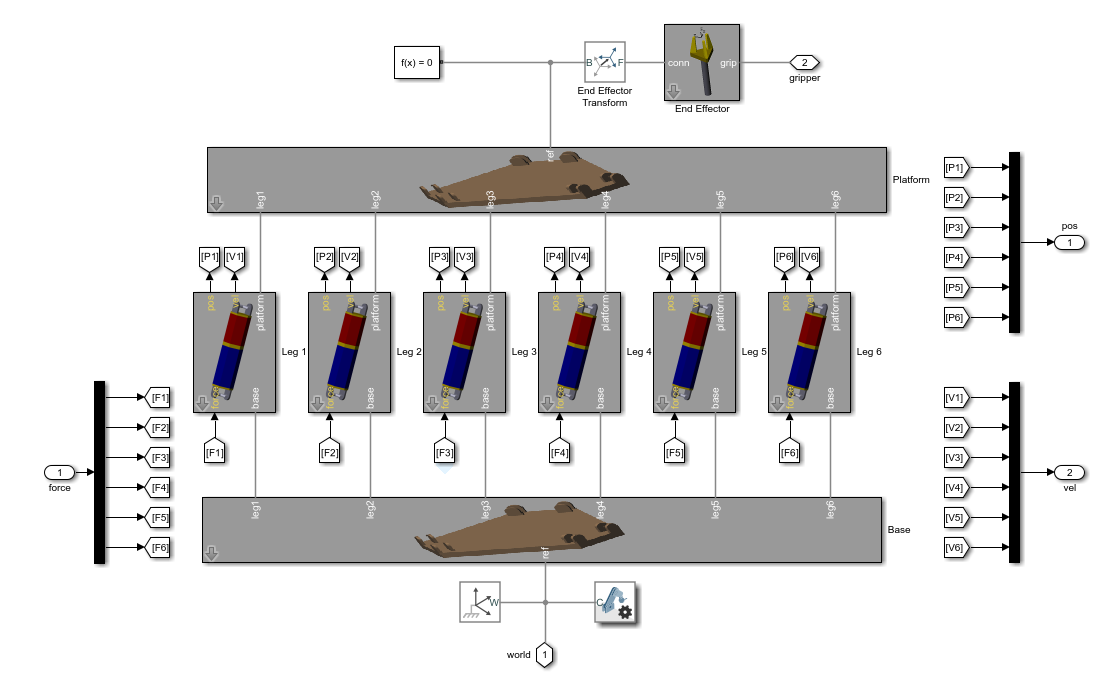
\includegraphics[width=1\columnwidth]{Figures/stewart_simulink2.png}
        \caption{Bloques internos del modelo mecánico.}
        \label{fig:sim_slk_general3}
    \end{subfigure}
    \caption{Bloques de simulación Matlab/Simulink para plataforma Stewart.}
    \label{fig:sim_slk_general}
\end{figure}

%%%%%%%%%%%%%%% FIGURA PUNTO DE OPERACION %%%%%%%%%%%%%%%%%%%%%
\begin{figure}[H]
    \centering
    \begin{subfigure}[b]{\textwidth}
        \centering
        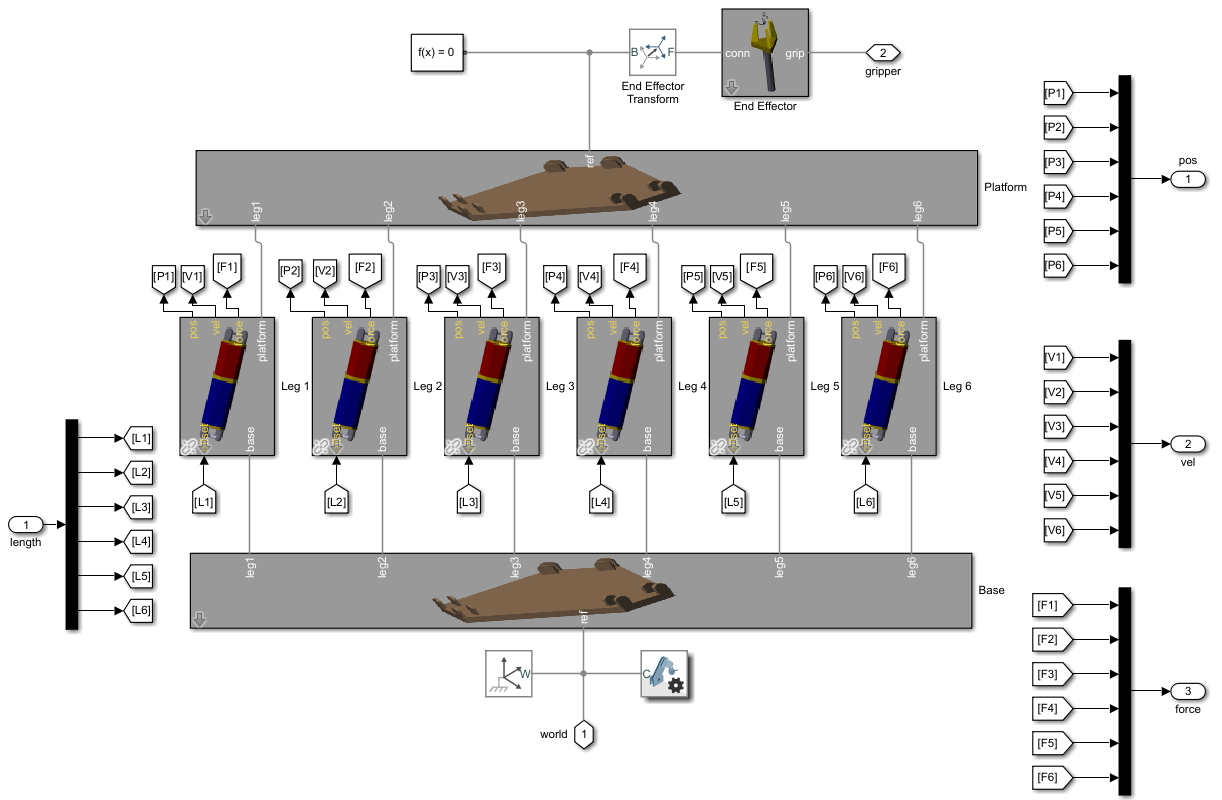
\includegraphics[width=0.85\columnwidth]{Figures/sim_slk_eq_general.png}
        \caption{Bloque general modificado del modelo mecánico para obtención del punto de operación.}
        \label{fig:sim_slk_eq_general}
    \end{subfigure}
    \hfill
    \begin{subfigure}[b]{\textwidth}
       \centering
        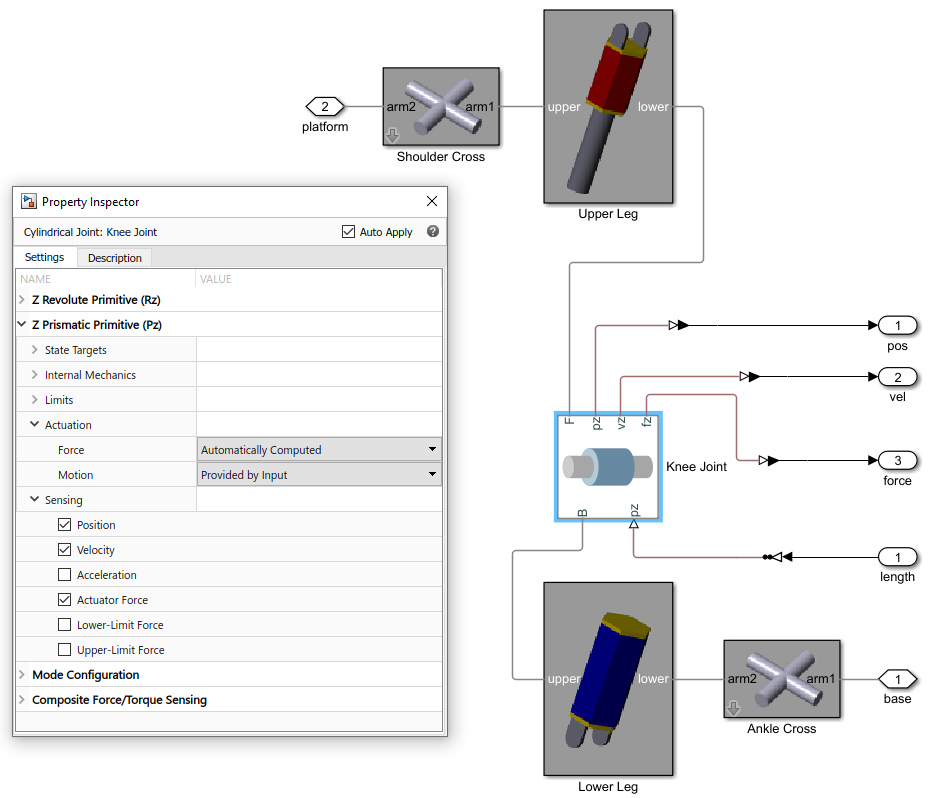
\includegraphics[width=0.7\columnwidth]{Figures/sim_slk_eq_legconfig.png}
        \caption{Configuración brazos actuadores para obtención del punto de operación.}
        \label{fig:sim_slk_eq_legconfig}
    \end{subfigure}
    \caption{Bloques de simulación Matlab/Simulink modificados para obtención del punto de operación.}
    \label{fig:sim_slk_eq}
\end{figure}


\subsection{Linealización}

Una vez obtenido el punto de operación, se procede a la linealización del sistema no lineal. Para esto, se utiliza una función llamada \textit{linmod()} que recibe como argumentos la Figura del bloque Simulink del modelo mecánico original \ref{fig:sim_slk_general1} y el punto de operación $(l_{EQ},\tau_{EQ})$ obtenido anteriormente.

De esta forma, se obtiene el modelo linealizado de la plataforma Stewart en formato de variables de estados: 
\begin{subequations} \label{eq:sys_varestados_original}
    \begin{align}
        \Dot{x}(t) & = A x(t) + B u(t), \\
        y(t) & = C x(t) + D u(t)
    \end{align}    
\end{subequations}

donde el vector de estados esta ordenado como $x(t) = \begin{bmatrix} x_1(t) & \dot{x}_1(t) & \hdots & x_6(t) & \dot{x}_6(t) \end{bmatrix}^{\top}$, el vector de entrada es de la forma $u(t) = \begin{bmatrix} u_1(t) & \hdots & u_6(t) \end{bmatrix}^{\top}$ y las matrices $A,B,C,D$ son

\begin{equation}
    A = \scalebox{0.95}{$\begin{bmatrix}
        0 &	1 &	0 &	0 &	0 &	0 &	0 &	0 &	0 &	0 &	0 &	0 \\
        32.623 & 0 & 18.85 & 0 & \textrm{-}12.29 & 0 & 8.51 & 0 & 32.49 & 0 & 25.75 & 0 \\
        0 &	0 &	0 &	1 &	0 &	0 &	0 &	0 &	0 &	0 &	0 &	0 \\
        19.83 &	0 &	28.61 &	0 &	1.27 &	0 &	17.93 &	0 &	28.20 &	0 &	30.97 &	0 \\
        0 &	0 &	0 &	0 &	0 &	1 &	0 &	0 &	0 &	0 &	0 &	0 \\
        \textrm{-}10.66 & 0 & 17.56 & 0 & 56.32 & 0 & \textrm{-}12.49 & 0 & \textrm{-}29.41 & 0 & 20.13 & 0 \\
        0 &	0 &	0 &	0 &	0 &	0 &	0 &	1 &	0 &	0 &	0 &	0 \\
        \textrm{-}5.19 &	0 &	\textrm{-}6.83 &	0 &	\textrm{-}7.23 &	0 &	75.76 &	0 &	9.66 &	0 &	24.39 &	0 \\
        0 &	0 &	0 &	0 &	0 &	0 &	0 &	0 &	0 &	1 &	0 &	0 \\
        3.08 & 0 & 9.72 & 0 & \textrm{-}2.61 & 0 & \textrm{-}13.57 & 0 & 34.10 & 0 & 0.69 & 0 \\
        0 &	0 &	0 &	0 &	0 &	0 &	0 &	0 &	0 &	0 &	0 &	1 \\
        6.56 & 0 & 3.36 & 0 & 10.21 & 0 & \textrm{-}4.67 & 0 & \textrm{-}0.23 & 0 & 35.91 & 0 \\
    \end{bmatrix}$}
\end{equation}

\begin{equation}
    B = \scalebox{0.95}{$\begin{bmatrix}
        0 &	0 &	0 &	0 &	0 &	0 \\
        0.070 &	0.333 &	\textrm{-}0.658 & \textrm{-}0.465 & 0.436 & 0.673 \\
        0 &	0 &	0 &	0 &	0 &	0 \\
        \textrm{-}0.333 &	\textrm{-}0.070 &	\textrm{-}0.673 &	\textrm{-}0.436 &	0.465 &	0.658 \\
        0 &	0 &	0 &	0 &	0 &	0 \\
        \textrm{-}0.658 &	\textrm{-}0.465 &	0.436 & 0.673 &	0.070 &	0.333 \\
        0 &	0 &	0 &	0 &	0 &	0 \\
        \textrm{-}0.172 &	\textrm{-}0.391 &	\textrm{-}0.115 &	\textrm{-}0.440 & 0.734 &	0.452 \\
        0 &	0 &	0 &	0 &	0 &	0 \\
        \textrm{-}0.062 &	0.200 &	\textrm{-}0.108 &	0.144 &	\textrm{-}7.770\cdot10^{\textrm{-}4} &	\textrm{-}0.012 \\
        0 &	0 &	0 &	0 &	0 &	0 \\
        \textrm{-}0.200 & 0.062 &	0.012 &	7.770\cdot10^{\textrm{-}4} &	\textrm{-}0.144 &	0.108 \\
    \end{bmatrix}$}
\end{equation}

\begin{equation}
    C = \scalebox{0.9}{$\begin{bmatrix}
        32.55 &	0 &	\textrm{-}30.03 &	0 &	2.52  &	0 &	\textrm{-}1.16 &	0 &	\textrm{-}14.14 &	0 &	\textrm{-}12.74  &	0 \\
        30.10 &	0 &	\textrm{-}33.33 &	0 &	0.63  &	0 &	3.35           &	0 &	13.19            &	0 &	13.91            &	0 \\
        15.43 &	0 &	\textrm{-}36.79 &	0 &	7.75  &	0 &	17.96          &	0 &	16.71            &	0 &	13.40            &	0 \\
        15.14 &	0 &	\textrm{-}21.18 &	0 &	15.64 &	0 &	2.74           &	0 &	19.15            &	0 &	\textrm{-}9.84   &	0 \\
        19.45 &	0 &	\textrm{-}19.23 &	0 &	10.40 &	0 &	15.32          &	0 &	11.66            &	0 &	\textrm{-}19.22  &	0 \\
        32.31 &	0 &	\textrm{-}16.24	&   0 &	15.88 &	0 &	\textrm{-}1.56 &	0 &	\textrm{-}14.071 &	0 &	\textrm{-}14.44  &	0 \\
        0 &	32.55 &	0 &	\textrm{-}30.03 &	0 &	2.52    & 0 &	\textrm{-}1.16  & 0 & \textrm{-}14.14  &	0 &	\textrm{-}12.74 \\
        0 &	30.10 &	0 &	\textrm{-}33.33	&   0 &	0.63    & 0 &	3.35	        & 0	& 13.19            &	0 &	13.91 \\
        0 &	15.43 &	0 &	\textrm{-}36.79 &	0 &	7.75	& 0 &	17.96	        & 0	& 16.71            &	0 &	13.40 \\
        0 &	15.14 &	0 &	\textrm{-}21.18 &	0 &	15.64	& 0 &	2.74	        & 0	& 19.15            &	0 &	\textrm{-}9.84 \\
        0 &	19.45 &	0 &	\textrm{-}19.23 &	0 &	10.40	& 0 &	15.32	        & 0	& 11.66            &	0 &	\textrm{-}19.22 \\
        0 &	32.31 &	0 &	\textrm{-}16.24 &	0 &	15.88	& 0 &	\textrm{-}1.56	& 0	& \textrm{-}14.07  &	0 &	\textrm{-}14.44 \\
    \end{bmatrix}$}
\end{equation}

\begin{equation}
    D = \scalebox{0.9}{$\begin{bmatrix}
        0 & \hdots & 0 \\
        \vdots & \ddots & \vdots \\
        0 & \hdots & 0
    \end{bmatrix}_{12\times6} $}
\end{equation}

El principal inconveniente de este modelo linealizado, es que los estados no son directamente medibles en la salida, ya que las salidas del sistema son una combinación de ellos. Debido a que los estados serán utilizados para el diseño de control, se propone realizar una transformación de similaridad al sistema linealizado, modificando los estados originales a la posición y velocidad correspondiente de cada brazo actuador, y así poder ser medidos directamente a la salida del sistema lineal para facilitar el proceso del diseño de control.


\subsection{Transformación de Similaridad}

La transformación de similaridad al sistema en variables de estados se utiliza de tal forma de poder medir directamente los estados internos del sistema a la salida del mismo. 

\begin{mybox}{}
    \begin{lemma} \label{lem3:sys_transform}
        Sea el sistema lineal \ref{eq:sys_varestados_original} en variables de estados de la plataforma Stewart, se define el sistema lineal con transformación de similaridad como:
        \begin{subequations} \label{eq:sys_varestados_transf}
            \begin{align}
                \Dot{\xi}(t) & = A_0 \cdot \xi(t) + B_0 \cdot u(t), \\
                y(t) & = C_0 \cdot \xi(t) + D_0 \cdot u(t)
            \end{align}    
        \end{subequations}
        
        donde\\ \scalebox{0.95}{$A_0 = CAC^{-1} = \begin{bmatrix}
                0_{6\times6} & I_{6\times6} \\ \Phi & 0_{6\times6}
            \end{bmatrix}, \hspace{0.2cm}
            B_0 = CB = \begin{bmatrix}
                0_{6\times6} \\ \Gamma
            \end{bmatrix}, \hspace{0.2cm} 
            C_0 = CC^{-1} = I_{12\times12}, \hspace{0.2cm}
            D_0 = D = 0_{12\times6}$}
        
        con $I$ la matriz identidad.
    \end{lemma}
\end{mybox}




\begin{proof}

En primera instancia, se necesita que la matriz $C$ del sistema lineal original \ref{eq:sys_varestados_original} sea invertible. Mediante el comando \textit{det(C)} se obtiene un determinante igual a $\textrm{-}2.54\cdot10^{16}$ distinto de cero, por ende, la matriz $C$ de \ref{eq:sys_varestados_original} si es invertible.

Considerando la matriz $C$ como matriz de transformación, se define un nuevo estado del sistema:
\begin{equation}
    \xi(t) = C \cdot x(t)
\end{equation}

Multiplicando por la izquierda al estado del sistema en \ref{eq:sys_varestados_original} con la matriz $C$ de transformación, y considerando el estado original como $x(t)=C^{-1}\cdot \xi(t)$, se desarrolla:

\begin{subequations}
\begin{align}
    C \dot{x}(t) & = CA \cdot x(t) + CB \cdot u(t) \notag \\   
    \Longrightarrow \dot{\xi}(t) & = \underbrace{CAC^{-1}}_{A_0} \cdot \xi(t) + \underbrace{CB}_{B_0} \cdot u(t) \\
    \notag \\
    y(t) & = C \cdot x(t) + D \cdot u(t) \notag \\
    \Longrightarrow y(t) & = \underbrace{CC^{-1}}_{C_0} \cdot \xi(t) + \underbrace{D}_{D_0} \cdot u(t)
\end{align}
\end{subequations}

\end{proof}

Las matrices $\Phi$ y $\Gamma$ del Lema \ref{lem3:sys_transform} son:
        
\begin{equation}    
\Phi = \begin{bmatrix}
    43,47 & \textrm{-}2,81 & \textrm{-}14,58 & 0,35 & 9,43 & \textrm{-}30,20 \\
    \textrm{-}2,83 &	43,44 &	\textrm{-}30,18 & 9,46 &	0,34 &	\textrm{-}14,56 \\
    9,12 & \textrm{-}31,05 &	44,25 &	\textrm{-}2,36 &	\textrm{-}14,80 & 0,48 \\
    \textrm{-}0,09 &	\textrm{-}15,26 & \textrm{-}2,13 & 44,09 & \textrm{-}30,61 & 9,60 \\
    \textrm{-}15,28 & \textrm{-}0,20 & 9,66 &	\textrm{-}30,39 & 43,91 & \textrm{-}2,09 \\
    \textrm{-}30,91 & 9,18 &	0,42 & \textrm{-}14,64 &	\textrm{-}2,57 & 44,18 \\
\end{bmatrix}
\end{equation}

\begin{equation}
\Gamma = \begin{bmatrix}
    14,29 &	8,62 &	1,42 &	\textrm{-}1,86 &	1,42 &	1,28 \\
    8,62 &	14,29 &	1,28 &	1,42 &	\textrm{-}1,86 &	1,42 \\
    1,42 &	1,28 &	14,29 &	8,62 &	1,42 &	\textrm{-}1,86 \\
    \textrm{-}1,86 &	1,42 &	8,62 &	14,29 &	1,28 &	1,42 \\
    1,42 &	\textrm{-}1,86 &	1,42 &	1,28 &	14,29 &	8,62 \\
    1,28 &	1,42 &	\textrm{-}1,86 &	1,42 &	8,62 &	14,29 \\
\end{bmatrix}
\end{equation}

\newpage
El sistema lineal transformado \eqref{eq:sys_varestados_transf} del Lema \ref{lem3:sys_transform} posee la particularidad que el vector de estados fue modificado. Estos estados modificados ahora son directamente la longitud y velocidad respectiva de cada brazo actuador, ordenados de la siguiente manera:
        \begin{align} \label{eq:sys_estados}
            \xi (t) & = \begin{bmatrix}
                l(t)^{\top} & \dot{l}(t)^{\top}
            \end{bmatrix}^{\top} \notag \\
            & = \begin{bmatrix}
                l_1(t) & \hdots & l_6(t) & \dot{l}_1(t) & \hdots & \dot{l}_6(t)
            \end{bmatrix}^{\top}
        \end{align}

%##############################################################
%##############################################################

\section{Análisis del Modelo Linealizado}
\lhead[\thepage]{Sección \thesection. Análisis modelo linealizado}

Con el sistema lineal transformado de la plataforma Stewart obtenido en \ref{eq:sys_varestados_transf} en forma de variables de estados, se utiliza su representación en función de transferencia $G(s)$ para el análisis MIMO del sistema, con la diferencia de tener solo las posiciones de los brazos como salida medible $(G(s)_{6\times6})$, para facilitar el análisis del modelo. 

Evaluando el sistema $G(s)_{6\times6}$ en $s=\infty$ se obtiene una matriz de ceros. Esto nos indica que el sistema lineal obtenido de la plataforma Stewart es estrictamente propio. Que sea estrictamente propio es un buen indicio ya que permitirá tener un mejor manejo de la respuesta del sistema frente a perturbaciones o cambios en la entrada, además de posiblemente no tener comportamientos indeseados a altas frecuencias que perturben el control del sistema.
\begin{equation}
    G(\infty)_{6\times6} = 0_{6\times6}
\end{equation}

Se obtuvieron los polos del sistema $G(s)_{6\times6}$ mostrados a continuación, evidenciándose tanto polos estables como inestables. Por otro lado, también se muestran los ceros de cada función de transferencia SISO presente en $G(s)_{6\times6}$:

\begin{equation}\label{eq:polos_stewart}
    polos = \begin{bmatrix}
        -8.440 \\ -8.214 \\ -8.200 \\ -5.094 \\ -5.077 \\ -2.376 \\
        2.376 \\ 5.077 \\ 5.094 \\ 8.200 \\ 8.214 \\ 8.440
    \end{bmatrix} 
\end{equation}
\begin{equation} \label{eq:ceros_stewart}
    ceros_{SISO} = \scalebox{0.9}{$\begin{bmatrix}
       -8.4409                  \\
       -8.4254   \pm 0.0045 i   \\
       -8.2544                  \\
       -8.2208   \pm 0.0595 i   \\
       -8.2142                  \\
       -8.2017   \pm 0.0788 i   \\
       -8.2001                  \\
       -8.1692                  \\
       -5.1177                  \\
       -5.0896   \pm 0.0074 i   \\
       -5.0767                  \\
       -2.3860                  \\
        2.3860                  \\
        5.0767                  \\
        5.0896   \pm 0.0074 i   \\
        5.1177                  \\
        8.1692                  \\
        8.2001                  \\
        8.2017   \pm 0.0788 i   \\
        8.2128                  \\
        8.2208   \pm 0.0595 i   \\
        8.2544                  \\
        8.4254   \pm 0.0045 i   \\
        8.4408                  \\
    \end{bmatrix} $}
\end{equation}

Recordando sobre los ceros multivariables (MIMO), estos deben tener la característica de que al ser evaluados en la función de transferencia $G(s)_{6\times6}$, esta función debe perder rango completo en filas o columnas. Si evaluamos todos los ceros SISO obtenidos anteriormente en $G(s)_{6\times6}$ notaremos que ningún cero SISO hace perder rango completo a la función de transferencia. Es por esto que no se posee ningún cero MIMO en el sistema.

Sea la matriz de arreglo de ganancias relativas, definida como $\Lambda_{RGA}(s) = G(s)\odot \left[ G(s)^{-1} \right]^\top$, podemos encontrar la relación de las entradas $u$ con las salidas $y$ del sistema. Evaluando para frecuencia cero, es decir $s=0$, se obtiene:
\begin{equation} 
    \Lambda_{RGA}(0) = \begin{bmatrix}
        6.116 &  \textrm{-}3.373 &  \textrm{-}0.669 &   1.129 & \textrm{-}0.641  & \textrm{-}1.560 \\
       \textrm{-}3.368 &  6.078  &  \textrm{-}1.544 &  \textrm{-}0.634 & 1.134   & \textrm{-}0.665 \\
       \textrm{-}0.694 &  \textrm{-}1.623 &   5.926 &  \textrm{-}3.148 & \textrm{-}0.687  &  1.227 \\
        1.273 &  \textrm{-}0.667 &  \textrm{-}3.253 &   5.796 & \textrm{-}1.441  & \textrm{-}0.708 \\
       \textrm{-}0.692 &   1.243 &  \textrm{-}0.641 &  \textrm{-}1.488 & 5.807   & \textrm{-}3.228 \\
       \textrm{-}1.634 &  \textrm{-}0.657 &   1.183 &  \textrm{-}0.655 & \textrm{-}3.171  & 5.936 \\
    \end{bmatrix}
\end{equation}

La matriz RGA obtenida cumple con las propiedades necesarias que son $\sum_{\textit{fila i}} = 1$ y $\sum_{\textit{columna i}} = 1$ para $i = 1,\hdots,6$. Con estas propiedades cumplidas, es posible notar una correspondencia uno a uno entre las entradas $u$ y las salidas $y$, es decir, una alineación directa, estableciendo así los siguientes emparejamientos entre las entradas y salidas:
\begin{align*}
    u_1 \rightarrow y_1 \\
    u_2 \rightarrow y_2 \\
    u_3 \rightarrow y_3 \\
    u_4 \rightarrow y_4 \\
    u_5 \rightarrow y_5 \\
    u_6 \rightarrow y_6 \\
\end{align*}

Es por esto que, una opción de diseño de controlador descentralizado para la plataforma Stewart si lograría ser capaz de controlar el sistema. 

En el capítulo \ref{cap:mimoPID} se analizará de forma detallada una comparación entre un control MIMO PID full con versiones descentralizadas del mismo, buscando el control más adecuado para el sistema.



% =========================== CAPÍTULO 4 ============================ %
\lhead[\thepage]{\thechapter. \rightmark}
\rhead[\leftmark]{\thepage}
\renewcommand{\headrulewidth}{0.5pt}
\lfoot[]{}
\cfoot[]{}
\rfoot[]{}
\renewcommand{\footrulewidth}{0pt}
	
\fancypagestyle{plain}{
	\fancyhead[L]{}
	\fancyhead[C]{}
	\fancyhead[R]{\thepage}
	\fancyfoot[L]{}
	\fancyfoot[C]{}
	\fancyfoot[R]{}
	\renewcommand{\headrulewidth}{0.5pt}
}
	\chapter{DISEÑO DE CONTROL MIMO PID SINTETIZADO POR CONTROL LQI}
\label{cap:mimoPID} 
\renewcommand{\proofname}{Demostración}
\markboth{CAPÍTULO \thechapter. DISEÑO DE CONTROL MIMO PID}{CAPÍTULO \thechapter. DISEÑO DE CONTROL MIMO PID}

En este capítulo se desarrolla el diseño de control de la plataforma Stewart, caracterizado por ser un control MIMO PID sintetizado mediante un control LQI. Además, se desarrolla una versión descentralizada del controlador MIMO PID para ser optimizado mediante un algoritmo numérico. Los controladores desarrollados son simulados y comparados mediante tablas bajo distintos índices de desempeño.

%##############################################################
%##############################################################
\section{Diseño de controlador LQI para plataforma Stewart}
\lhead[\thepage]{Sección \thesection. Diseño control LQI}
\label{sec:lqi_stewart}

Se considera el sistema lineal transformado de la plataforma Stewart en \ref{eq:sys_varestados_transf}, con la diferencia de una matriz $C$ dada por $C_{pos}=\begin{bmatrix} I_{6\times6} & 0_{6\times6}\end{bmatrix}$. Esto quiere decir, que únicamente se tendrá como medición disponible del sistema las posiciones de los brazos, es decir, los primeros 6 estados internos de $\xi(t)$ mostrados en \ref{eq:sys_estados}. Además, se considera el diseño de control LQI presentado en el Capítulo \ref{cap:Notación y preliminares}. El diseño de control LQI se centrará en seguir a la referencia $r(t)$ definida únicamente con las posiciones deseadas de los brazos actuadores.  

Se define la ley de control para el estado aumentado $z(t)=\begin{bmatrix} \xi(t)^{\top} & \xi_{int}(t)^{\top} \end{bmatrix}^{\top}$ donde $\xi(t)$ son los estados internos del sistema lineal transformado denotados como $\xi(t) = \begin{bmatrix} l(t)^{\top} & \dot{l}(t)^{\top} \end{bmatrix}^{\top}$, y con $\xi_{int}(t)$ el nuevo estado definido como la integral del error de posición $\left(\xi_{int}(t)=\int r(t) - C_{pos} \xi(t)\right)$:

\begin{align}
    u^*(t) & = - K_z \cdot z(t) \notag \\
    & = -K_{pos} l(t) - K_{vel} \dot{l}(t) - K_{int} \xi_{int}(t)
\end{align}
donde $K_z = \begin{bmatrix} K_{pos} & K_{vel} & K_{int} \end{bmatrix}$ es la matriz de realimentación LQI.


%##############################################################
%##############################################################
\section{Diseño de controlador MIMO PID mediante control LQI}
\lhead[\thepage]{Sección \thesection. Diseño control MIMO PID}
\label{sec:mimopid_stewart}

Se considera el sistema lineal transformado de \ref{eq:sys_varestados_transf}, con su matriz $C$ original ($C_0$), es decir, con las salidas medibles disponibles de la posición y la velocidad de los brazos. 

Se posee una estructura general de un controlador PID, con las matrices $K_P$, $K_D$ y $K_I$ como las ganancias de proporcionalidad, derivativas y de integración respectivamente. 

Como la velocidad de la referencia es conocida, es posible desarrollar la actuación del sistema con el error de posición $ e(t) = r(t) - l(t)$ y el error de velocidad $\dot{e}(t) = \dot{r}(t) - \dot{l}(t)$

\begin{align} \label{eq:actuacion_pid}
    u(t) & = K_P e(t) + K_D \dot{e}(t) + K_I \frac{e(t)}{s} \notag \\
    & = K_P r(t) - K_P l(t) + K_D \dot{r}(t) - K_D \dot{l}(t) + K_I \frac{r(t)}{s} - K_I \frac{l(t)}{s}
\end{align}

De la sección anterior, se obtuvo la ley de control LQI dada por la actuación:
\begin{equation} \label{eq:actuacion_lqi}
    u(t) = -K_{pos} l(t) - K_{vel} \dot{l}(t) - K_{int} \frac{e(t)}{s}
\end{equation}

Comparando ambas actuaciones \ref{eq:actuacion_pid} y \ref{eq:actuacion_lqi}, se puede notar que para lograr una misma actuación, se necesita de un \textit{feedforward} en el controlador MIMO PID. El feedforward necesario para la actuación esta dado por $-K_P r(t) - K_D \dot{r}(t)$.

\begin{mybox}{}
    \begin{lemma} \label{lem4:mimo_pid}
        Se define el controlador MIMO PID con feedforward sintetizado por control LQI como:
        \begin{equation} \label{eq:actuacion_mimopid}
            u^*(t) = \left( K_P e(t) + K_D \dot{e}(t) + K_I \frac{e(t)}{s} \right) - K_P r(t) - K_D \dot{r}(t)
        \end{equation}
        
        con las ganancias $K_P$, $K_D$ y $K_I$ del controlador MIMO PID definidas por las ganancias de realimentación LQI $K_{pos}$, $K_{vel}$ y $K_{int}$:
        \begin{equation} \label{eq:gain_comparative_lqi_pid}
            K_P = K_{pos}, \qquad K_D = K_{vel}, \qquad K_I = -K_{int}
        \end{equation}
    \end{lemma}
\end{mybox}

En la Figura \ref{fig:pid_scheme} se ilustra el esquema de control MIMO PID con feedforward desarrollado.\\

Los controladores MIMO PID son poco comunes en la industria, y no es claro cuanto es la mejora real que pueden otorgar en comparación con los controladores PID descentralizados, los cuales son ampliamente usados. En las secciones siguientes se definirán controladores descentralizados para ser comparados con el MIMO PID desarrollado.

\begin{figure}[ht]
\centering
    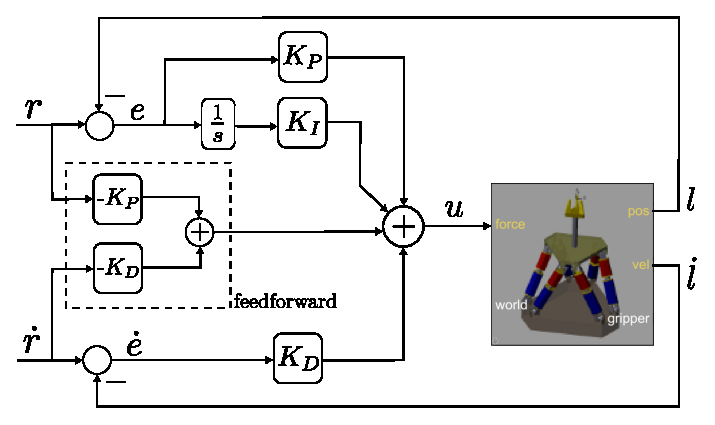
\includegraphics[width=0.7\columnwidth]{Figures/MIMO_PID/mimo_pid_scheme.eps}
    \caption{Esquema de control MIMO PID con feedforward para la plataforma Stewart.}
    \label{fig:pid_scheme}
\end{figure}

%##############################################################
%##############################################################
\section{Descentralización de controlador MIMO PID y optimización de desempeño}
\lhead[\thepage]{Sección \thesection. Diseño de control MIMO PID Descentralizado}
\label{sec:mimopid_descentralizado_stewart}

A partir del controlador MIMO PID obtenido anteriormente, se desarrolla la descentralización del PID junto a un algoritmo de optimización de desempeño, obteniéndose 2 tipos de controladores PID descentralizados para su posterior comparación con el controlador MIMO PID.

\subsection{Controlador PID descentralizado}

Considerando el controlador MIMO PID con feedforward de \ref{eq:actuacion_mimopid}, se define el controlador PID descentralizado con feedforward removiendo los términos fuera de la diagonal de las matrices $K_P$, $K_D$ y $K_I$, de la forma

\begin{equation} \label{eq:gain_lqi_desc}
    K_P^0 = K_P \odot I, \qquad K_D^0 = K_D \odot I, \qquad K_I^0 = K_I \odot I 
\end{equation}
donde $I$ es la matriz identidad y $\odot$ denota al producto de Hadamard.

\begin{remark}
    Se utiliza el sobrescrito $^0$ para representar las correspondientes matrices del controlador descentralizado inicial, diferenciándose con su versión descentralizada optimizada desarrollada a continuación con el sobrescrito $^N$, con $N$ el número de iteraciones del algoritmo de optimización.
\end{remark}

\subsection{Optimización PID descentralizado}

Para la optimización del controlador PID descentralizado obtenido anteriormente, se utiliza un algoritmo numérico de \cite{silva2006lqr}. Este algoritmo emplea como técnica un simple descenso del gradiente que converge iterativamente en una solución descentralizada óptima para problemas de control LQR.

Para nuestro caso, se contempla el sistema aumentado \ref{eq:sys_aumentado_lqi} con el sistema lineal transformado \ref{eq:sys_varestados_transf} de la plataforma Stewart utilizado en el diseño de control LQI. Además se considera la matriz de realimentación LQI descentralizada con las ganancias obtenidas en \ref{eq:gain_lqi_desc}:
\begin{equation} \label{eq:gain_lqi_desc2}
    K_z^0 = \begin{bmatrix}
        K_P^0 & K_D^0 & -K_I^0
    \end{bmatrix}
\end{equation}
para la ley de control 
\begin{equation}
    u(t) = -K_z^0 \cdot z(t)
\end{equation}
con $z(t)=\begin{bmatrix} \xi(t)^{\top} & \xi_{int}(t)^{\top} \end{bmatrix}^{\top} = \begin{bmatrix} l(t)^{\top} & \dot{l}(t)^{\top} & \xi_{int}(t)^{\top} \end{bmatrix}^{\top}$ el estado aumentado del sistema.

Se deduce que la función objetivo LQR promediada del estado inicial estándar se puede escribir como:

\begin{equation}
    J(K) = \textrm{trace} \left\{ F(K) \right\}
\end{equation}
donde $F(K)$ es la función de coste LQR de la forma:
\begin{equation} \label{eq:costo_algorithm_F(K)}
    F(K) = \int_0^\infty \Lambda(t)^{\top} \left( \Psi + K^{\top} \Omega K \right) \Lambda(t) \quad dt
\end{equation}

con $\Lambda(t) = e^{(A_a+B_a K)t}$, $\Psi \geq 0$ y $\Omega > 0$. Se debe notar que como $A_a + B_a K$ es estable, es posible obtener $F(K)$ de otra forma, como la solución a la ecuación de Lyapunov siguiente:

\begin{equation} \label{eq:algorithm_F(K)}
    \left( A_a + B_a K \right)^{\top} F(K) + F(K) \left( A_a + B_a K \right) + \left( \Psi + K^{\top} \Omega K \right) = 0
\end{equation}

Se inicia con una solución estable dada por $K = K_0$ (en nuestro caso la solución inicial será $K_z^0$ definida en \ref{eq:gain_lqi_desc2}), para descender en dirección contraria al gradiente disminuyendo el valor del funcional de costo de la forma $K=K_0-\textit{dirección-contragradiente}$. Para esto se define el $i^{th}$ candidato $K$, tal que $K_i$:

\begin{equation}
    K_i = K_{i-1} - \mu \frac{d}{dK}\textrm{ trace}\left\{ F(K_{i-1}) \right\} \qquad i = 1,2,\hdots,N
\end{equation}

donde $N$ es el número de iteraciones y $\mu>0$ es un número real pequeño relacionado con la velocidad de convergencia y estabilidad del algoritmo. Es posible escribir la derivada de la traza como: 

\begin{equation}
    \frac{d}{dK} \textrm{ trace} \left\{F(K_i)\right\} = 2\left( \Omega K_i + B_a^{\top} F(K_i) \right) W
\end{equation}
con $F(K_i)$ definido en \ref{eq:costo_algorithm_F(K)} y \ref{eq:algorithm_F(K)}, y con $W$ la solución a la ecuación de Lyapunov:
\begin{equation}
    \left( A_a + B_a K_i \right) W + W \left( A_a + B_a K_i \right)^{\top} + I = 0
\end{equation}
con I la matriz identidad.

Es posible que el gradiente de $K=K_{i-1}$ no posea necesariamente la estructura deseada de la solución que se busca, ya que a medida que se desarrollan las iteraciones buscando un óptimo, puede que la estructura se pierda. Para prevenir esto se establece un operador $\textrm{sp}\{\cdot\}$ encargado de conservar la estructura deseada, que en nuestro caso se basa en diagonalizar el gradiente, para así mantener la estructura descentralizada que se busca. Dada una matriz $X$ se define el operador $\textrm{sp}\{\cdot\}$:

\begin{equation}
    \textrm{sp} \left\{ X \right\} = X \odot \begin{bmatrix}
        I & I & I
    \end{bmatrix}
\end{equation}

con $I$ matrices identidad de dimensiones apropiadas. De esta forma es posible actualizar la ecuación de optimización descentralizada como:

\begin{equation}
    K_i = K_{i-1} - \mu \textrm{ sp} \left\{\frac{d}{dK}\textrm{ trace}\left\{ F(K_{i-1}) \right\} \right\} 
\end{equation}

El algoritmo descrito preserva la estructura deseada del controlador en cada iteración, pero la estabilidad del mismo puede perderse. Para solucionar esto, se debe verificar la estabilidad del controlador previo a cada actualización, descartando los controladores $K_i$ que no son estables. Escogiendo un valor de $\mu$ suficientemente pequeño se garantiza no perder estabilidad en el controlador iterado.



%##############################################################
%##############################################################
\newpage
\section{Resultados de simulación MIMO PID}
\lhead[\thepage]{Sección \thesection. Resultados de simulación MIMO PID}
\label{sec:resultados_mimoPID}

Los resultados de los distintos controladores son comparados mediante índices de desempeño en tablas comparativas. Estos índices de desempeño se definen como la integral del error cuadrático ($J_{ISE}$), el esfuerzo de control definido por la integral de la actuación cuadrática ($J_u$), y la función de costo LQI ($J_{LQI}$). Se muestra a continuación la definición de los respectivos índices de desempeño:
\begin{align} \label{eq:indices_desempeño}   
    J_{ISE} & = \int_0^{T_{sim}} e(t)^\top e(t) dt, \\ 
    J_{u} & = \int_0^{T_{sim}} u(t)^\top u(t) dt,\\
    J_{LQI} & =\int_0^{T_{sim}} \left( z(t)^{\top}Qz(t) + u(t)^{\top}Ru(t) \right) \ dt
\end{align}
con $T_{sim}$ el tiempo de simulación y $z(t)=\begin{bmatrix} \xi(t)^{\top} & \xi_i(t)^{\top} \end{bmatrix}^{\top}$ el estado aumentado. Se debe destacar que se utiliza $S=0$ para la función de coste genérica LQI descrita en el capítulo \ref{cap:Notación y preliminares}, obteniendo así el coste $J_{LQI}$ recién mencionado.

Se establecen 2 casos a estudiar, para distintos valores de las matrices $Q$ y $R$ en la obtención de la matriz de realimentación LQI para el diseño de control MIMO PID. La matriz de realimentación se obtiene mediante el comando \textit{lqi()} con el sistema lineal transformado \ref{eq:sys_varestados_transf} y $C_{pos}$, definido en la sección \ref{sec:lqi_stewart}.

En todos los casos estudiados, los parámetros del algoritmo de optimización utilizados para el controlador descentralizado son $\mu=5\cdot 10^{-4}$ y $N=1000$ iteraciones para la tasa de convergencia. Mediante experimentación se encontró que estos valores son suficientes para observar una convergencia en el algoritmo de optimización.

\subsubsection{Caso 1:}
Para el Caso 1 los parámetros en la obtención de la matriz de realimentación LQI son:
\begin{equation}
    Q = I_{18\times18}, \qquad R = 0.1\cdot I_{6\times6}
\end{equation}
con $I$ la matriz identidad. La matriz $Q$ identidad pondera a todos los estados por igual. Por otro lado con la matriz $R$ se penaliza levemente la actuación de entrada para así no restringir tanto su efecto en el sistema.

Las matrices del controlador MIMO PID sintetizadas por diseño de control LQI en la sección \ref{sec:mimopid_stewart} son:

\begin{equation}
    K_P = \begin{bmatrix}
        15.164&	\textrm{-}6.499&	\textrm{-}2.054&	4.022&	\textrm{-}1.492&	\textrm{-}3.397 \\
        \textrm{-}6.506&	15.134&	\textrm{-}3.391&	\textrm{-}1.473&	4.016&	\textrm{-}2.036 \\
        \textrm{-}1.471&	\textrm{-}3.436&	15.206&	\textrm{-}6.506&	\textrm{-}2.052&	4.017 \\
        3.994&	\textrm{-}2.072&	\textrm{-}6.496&	15.222&	\textrm{-}3.443&	\textrm{-}1.465 \\
        \textrm{-}2.100&	3.975&	\textrm{-}1.447&	\textrm{-}3.434&	15.232&	\textrm{-}6.485 \\
        \textrm{-}3.423&	\textrm{-}1.451&	4.009&	\textrm{-}2.053&	\textrm{-}6.515&	15.191 \\
    \end{bmatrix}
\end{equation}

\begin{equation}
    K_D = \begin{bmatrix}
        3.890&	\textrm{-}0.567&	\textrm{-}0.279&	0.395&	\textrm{-}0.133&	\textrm{-}0.072 \\
        \textrm{-}0.565&	3.888&	\textrm{-}0.073&	\textrm{-}0.132&	0.394&	\textrm{-}0.278 \\
        \textrm{-}0.132&	\textrm{-}0.073&	3.891&	\textrm{-}0.567&	\textrm{-}0.279&	0.396 \\
        0.396&	\textrm{-}0.280&	\textrm{-}0.568&	3.892&	\textrm{-}0.074&	\textrm{-}0.132 \\
        \textrm{-}0.281&	0.397&	\textrm{-}0.131&	\textrm{-}0.074&	3.893&	\textrm{-}0.568 \\
        \textrm{-}0.074&	\textrm{-}0.132&	0.396&	\textrm{-}0.279&	\textrm{-}0.567&	3.890 \\
    \end{bmatrix}
\end{equation}

\begin{equation}
    K_I = -\begin{bmatrix}
	\textrm{-}3.159&	0.0008&	0.096&	0.0007&	\textrm{-}0.100&	\textrm{-}0.0008 \\
	\textrm{-}0.0009&	\textrm{-}3.159&	\textrm{-}1.64\cdot10^{\textrm{-}5}&	\textrm{-}0.100&	0.001& 0.096 \\
	\textrm{-}0.099&	0.0001&	\textrm{-}3.159&	\textrm{-}0.0004&	0.097&	9.11\cdot10^{\textrm{-}5} \\
	\textrm{-}0.0006&	0.097&	0.0004&	\textrm{-}3.159&	\textrm{-}0.0004&	\textrm{-}0.100 \\
	0.097&	\textrm{-}0.001&	\textrm{-}0.100&	0.0003&	\textrm{-}3.159&	0.001 \\
	0.0008&	\textrm{-}0.099&	\textrm{-}0.0001&	0.097&	\textrm{-}0.0009&	\textrm{-}3.159 \\
    \end{bmatrix}
\end{equation}

Las matrices del controlador MIMO PID Descentralizado de la sección \ref{sec:mimopid_descentralizado_stewart} para el Caso 1 son:

\begin{equation}
    K_P^0 = K_P \odot I, \qquad K_D^0 = K_D \odot I, \qquad K_I^0 = K_I \odot I
\end{equation}
donde $I$ es la matriz identidad y $\odot$ el producto de Hadamard.

Las matrices del Caso 1 para el controlador MIMO PID Descentralizado Optimizado mediante el algoritmo de optimización con 1000 iteraciones, mencionado en la sección \ref{sec:mimopid_descentralizado_stewart}, son:

\begin{equation}
    K_P^{1000} = \begin{bmatrix}
        15.0839 &	0 &	0 &	0 &	0 &	0 \\
        0 &	15.0540 &	0 &	0 &	0 &	0 \\
        0 &	0 &	15.1259 &	0 &	0 &	0 \\
        0 &	0 &	0 &	15.1423 &	0 &	0 \\
        0 &	0 &	0 &	0 &	15.1514 &	0 \\
        0 &	0 &	0 &	0 &	0 &	15.1113 \\
    \end{bmatrix}
\end{equation}

\begin{equation}
    K_D^{1000} = \begin{bmatrix}
        4.0673 &	0 &	0 &	0 &	0 &	0 \\
        0 &	4.0653 &	0 &	0 &	0 &	0 \\
        0 &	0 &	4.0693 &	0 &	0 &	0 \\
        0 &	0 &	0 &	4.0702 &	0 &	0 \\
        0 &	0 &	0 &	0 &	4.0708 &	0 \\
        0 &	0 &	0 &	0 &	0 &	4.0685 \\
    \end{bmatrix}
\end{equation}

\begin{equation}
    K_I^{1000} = -\begin{bmatrix}
    \textrm{-}3.5441 &	0 &	0 &	0 &	0 &	0 \\
    0 &	\textrm{-}3.5434 &	0 &	0 &	0 &	0 \\
    0 &	0 &	\textrm{-}3.5459 &	0 &	0 &	0 \\
    0 &	0 &	0 &	\textrm{-}3.5459 &	0 &	0 \\
    0 &	0 &	0 &	0 &	\textrm{-}3.5458 &	0 \\
    0 &	0 &	0 &	0 &	0 &	\textrm{-}3.5454 \\
    \end{bmatrix}
\end{equation}

\subsubsection{Caso 2:}
Para el Caso 2 los parámetros en la obtención de la matriz de realimentación LQI son:
\begin{equation}
    Q = \begin{bmatrix} C_0^\top C_0 & 0 \\ 0 & 100\cdot I_{6\times6} \end{bmatrix}, \qquad R = 0.1\cdot I_{6\times6} 
\end{equation}
con $C_0$ la matriz de salida del sistema linealizado transformado \ref{eq:sys_varestados_transf} e $I$ la matriz identidad. En este caso, en la matriz $Q$ los estados correspondientes a la integral del error son ponderados en mayor medida que los demás, para así darle más importancia al seguimiento de la referencia. Por otro lado, con la matriz $R$ bajamente ponderada, no se castiga en gran cantidad la actuación para así no restringir su efecto en el sistema.

Las matrices del controlador MIMO PID sintetizadas por diseño de control LQI en la sección \ref{sec:mimopid_stewart} son:

\begin{equation} \label{eq:KP_mimoPID}
    K_P = \begin{bmatrix}
        24.037 &	\textrm{-}6.357 &	\textrm{-}2.141 &	3.812 &	\textrm{-}1.493 &	\textrm{-}2.746 \\
        \textrm{-}6.363 &	24.013 &	\textrm{-}2.739 &	\textrm{-}1.479 &	3.807 &	\textrm{-}2.125 \\
        \textrm{-}1.478 &	\textrm{-}2.785 &	24.078 &	\textrm{-}6.361 &	\textrm{-}2.137 &	3.807 \\
        3.784 &	\textrm{-}2.159 &	\textrm{-}6.351 &	24.089 &	\textrm{-}2.786 &	\textrm{-}1.467 \\
        \textrm{-}2.181 &	3.768 &	\textrm{-}1.452 &	\textrm{-}2.777 &	24.093 &	\textrm{-}6.341 \\
        \textrm{-}2.773 &	\textrm{-}1.461 &	3.799 &	\textrm{-}2.136 &	\textrm{-}6.370 &	24.065 \\
    \end{bmatrix}
\end{equation}

\begin{equation} \label{eq:KD_mimoPID}
    K_D = \begin{bmatrix}
        4.150 &	\textrm{-}0.710 &	\textrm{-}0.304 &	0.443 &	\textrm{-}0.194 &	\textrm{-}0.038 \\
        \textrm{-}0.709 &	4.148 &	\textrm{-}0.038 &	\textrm{-}0.193 &	0.442 &	\textrm{-}0.303 \\
        \textrm{-}0.193 &	\textrm{-}0.038 &	4.158 &	\textrm{-}0.710 &	\textrm{-}0.304 &	0.443 \\
        0.444 &	\textrm{-}0.305 &	\textrm{-}0.711 &	4.151 &	\textrm{-}0.039 &	\textrm{-}0.193 \\
        \textrm{-}0.306 &	0.445 &	\textrm{-}0.192 &	\textrm{-}0.040 &	4.152 &	\textrm{-}0.711 \\
        \textrm{-}0.039 &	\textrm{-}0.192 &	0.443 &	\textrm{-}0.304 &	\textrm{-}0.710 &	4.150 \\
    \end{bmatrix}
\end{equation}

\begin{equation} \label{eq:KI_mimoPID}
    K_I = -\begin{bmatrix}
    	\textrm{-}31.611 &	0.005 &	0.577 &	0.004 &	\textrm{-}0.594 &	\textrm{-}0.005 \\
    	\textrm{-}0.005 &	\textrm{-}31.611 &	\textrm{-}0.0002 &	\textrm{-}0.594 & 0.012 & 0.576 \\
    	\textrm{-}0.588 &	0.0006 &	\textrm{-}31.611 &	\textrm{-}0.002 &	0.582 &	0.0005 \\
    	\textrm{-}0.004 &	0.584 &	0.002 &	\textrm{-}31.611 &	\textrm{-}0.002 &	\textrm{-}0.592 \\
    	0.583 &	\textrm{-}0.012 &	\textrm{-}0.593 &	0.002 &	\textrm{-}31.611 &	0.005 \\
    	0.005 &	\textrm{-}0.587 &	\textrm{-}0.0008 &	0.581 &	\textrm{-}0.005 &	\textrm{-}31.611 \\
    \end{bmatrix}
\end{equation}

Las matrices del controlador MIMO PID Descentralizado de la sección \ref{sec:mimopid_descentralizado_stewart} para el Caso 2 son:

\begin{equation}
    K_P^0 = K_P \odot I, \qquad K_D^0 = K_D \odot I, \qquad K_I^0 = K_I \odot I
\end{equation}
donde $I$ es la matriz identidad y $\odot$ el producto de Hadamard.

Las matrices del Caso 2 para el controlador MIMO PID Descentralizado Optimizado mediante el algoritmo de optimización con 1000 iteraciones, mencionado en la sección \ref{sec:mimopid_descentralizado_stewart}, son:

\begin{equation}
    K_P^{1000} = \begin{bmatrix}
        23.5097 &	0 &	0 &	0 &	0 &	0 \\
        0 &	23.4860 &	0 &	0 &	0 &	0 \\
        0 &	0 &	23.5490 &	0 &	0 &	0 \\
        0 &	0 &	0 &	23.5603 &	0 &	0 \\
        0 &	0 &	0 &	0 &	23.5639 &	0 \\
        0 &	0 &	0 &	0 &	0 &	23.5361 \\
    \end{bmatrix}
\end{equation}

\begin{equation}
    K_D^{1000} = \begin{bmatrix}
        3.7832 &	0 &	0 &	0 &	0 &	0 \\
        0 &	3.7813 &	0 &	0 &	0 &	0 \\
        0 &	0 &	3.7857 &	0 &	0 &	0 \\
        0 &	0 &	0 &	3.7866 &	0 &	0 \\
        0 &	0 &	0 &	0 &	3.7869 &	0 \\
        0 &	0 &	0 &	0 &	0 &	3.7848 \\
    \end{bmatrix}
\end{equation}

\begin{equation}
    K_I^{1000} = -\begin{bmatrix}
        \textrm{-}32.1930 &	0 &	0 &	0 &	0 &	0 \\
        0 &	\textrm{-}32.1922 &	0 &	0 &	0 &	0 \\
        0 &	0 &	\textrm{-}32.1953 &	0 &	0 &	0 \\
        0 &	0 &	0 &	\textrm{-}32.1952 &	0 &	0 \\
        0 &	0 &	0 &	0 &	\textrm{-}32.1950 &	0 \\
        0 &	0 &	0 &	0 &	0 &	\textrm{-}32.1948 \\
    \end{bmatrix}
\end{equation}



%%%%%%%%%%%%%%%%%%%%%%%%%%%%%%%%%%%%%%%%%%%%%%%%
\subsection{Referencia Escalón}

Se establece la señal de referencia para el movimiento de la plataforma superior por señales tipo escalón, donde en este caso describe un largo constante de brazos brindando una elevación fija a la plataforma superior:
\begin{equation} 
    q_{ref} = \begin{bmatrix}
        0 & 0 & 14 & 0 & 0 & 0
    \end{bmatrix}^{\top}
\end{equation}

Para un tiempo de simulación de $T_{sim}=50(s)$ se obtienen los resultados de los índices de desempeño mostrados en la tabla comparativa \ref{tab:indices_mimopid_escalon}:

\begin{table}[ht]
\centering
\begin{tabular}{c|c|c|c|c|}
\cline{2-5}
    & \textbf{PID MIMO} & $\mathbf{J_{ISE}}$ & $\mathbf{J_{u}}(\cdot10^5)$ & $\mathbf{J_{LQI}}(\cdot10^6)$ \\ \hline
\multicolumn{1}{|c|}{\multirow{3}{*}{Caso 1}} &  Full               & $2166$  & $3.5864$  & $0.4156$ \\ \cline{2-5} 
\multicolumn{1}{|c|}{}                        & Descentralizado 0   & $3367$  & $3.6082$  & $1.4256$ \\ \cline{2-5} 
\multicolumn{1}{|c|}{}                        & Descentralizado 1000& $3003$  & $3.6031$  & $1.1596$ \\ \hline
\multicolumn{1}{|c|}{\multirow{3}{*}{Caso 2}} & Full                & $399.1$ & $3.5660$  & $1.6167$ \\ \cline{2-5} 
\multicolumn{1}{|c|}{}                        & Descentralizado 0   & $516.6$ & $3.5687$  & $3.5093$ \\ \cline{2-5} 
\multicolumn{1}{|c|}{}                        & Descentralizado 1000& $496.9$ & $3.5687$  & $3.2593$ \\ \hline
\end{tabular}
\caption{Desempeño para PID MIMO Full y PID MIMO Descentralizado con $N=0$ y $N=1000$ iteraciones, referencia escalón.}
\label{tab:indices_mimopid_escalon}
\end{table}

Como se puede apreciar de la tabla \ref{tab:indices_mimopid_escalon} comparativa, para ambos casos se aprecia que el controlador MIMO PID Full posee los índices del error cuadrático ($J_{ISE}$) más bajos que los demás, siendo así mejores. Si usamos los índices del controlador MIMO PID Full como referencia, el controlador MIMO PID Descentralizado 0 muestra un $55.4\%$ de incremento del $J_{ISE}$ para el Caso 1 y un $29.4\%$ para el Caso 2. Siguiendo esta misma lógica, el controlador optimizado MIMO PID Descentralizado 1000 posee un incremento del $38.6\%$ para el Caso 1 y un $24.5\%$ para el Caso 2 del índice $J_{ISE}$, evidenciándose la mejoría del algoritmo de optimización al bajar el índice $J_{ISE}$ pero aun así sin poder igualar al MIMO PID Full.

Por otro lado, los valores del esfuerzo de control ($J_u$) son altos para ambos casos en todos los controladores. Tomando el controlador MIMO PID Full como referencia, el controlador MIMO PID Descentralizado 0 posee un aumento del $0.6\%$ para el Caso 1 y un $0.07\%$ para el Caso 2 en el índice $J_{u}$. Para el controlador optimizado MIMO PID Descentralizado 1000 este posee un $0.4\%$ en el Caso 1 y un $0.07\%$ para el Caso 2. Esta pequeña diferencia nos demuestra que el esfuerzo de control es casi el mismo para los 3 tipos de controladores, pero si se busca escoger el mejor sigue siendo el controlador MIMO PID Full.

Finalmente el índice de la función de coste LQI ($J_{LQI}$) muestra que el controlador MIMO PID Full es mejor que los demás al poseer los valores más pequeños de este índice. Al tomar este controlador MIMO PID Full como referencia para el índice $J_{LQI}$, podemos ver que la versión MIMO PID Descentralizado 0 posee un incremento del $243\%$ para el caso 1 y un $117\%$ para el Caso 2. Por otro lado el controlador optimizado MIMO PID Descentralizado 1000 posee un aumento del $179\%$ para el caso 1 y un $101.6\%$ para el Caso 2. 

Con esto, se demuestra la eficacia y el mejor desempeño en todos los ámbitos anteriores del controlador MIMO PID Full en comparación a sus versiones descentralizadas. 

En las Figuras \ref{fig:result_mimoPID_escalon_error1} y \ref{fig:result_mimoPID_escalon_fuerza1} se muestra el error de seguimiento y la fuerza aplicada respectivamente en cada brazo de la plataforma Stewart para el Caso 1. Se demuestra que el controlador MIMO PID Full posee un correcto seguimiento de la referencia, garantizando un error cero de seguimiento en estado estacionario. Sin embargo, las versiones descentralizadas comienzan a desestabilizarse a partir de los 30 segundos, apreciándose claramente en las gráficas de las fuerzas de los brazos. 

Con esto podemos deducir que para el Caso 1 las matrices $Q$ y $R$ escogidas nos limitan la velocidad de control, repercutiendo en que los controladores descentralizados no son capaces de estabilizar el sistema, siendo necesaria la versión MIMO PID Full para lograr un correcto control para la referencia tipo escalón. 
 
\begin{figure}[H]
\centering
    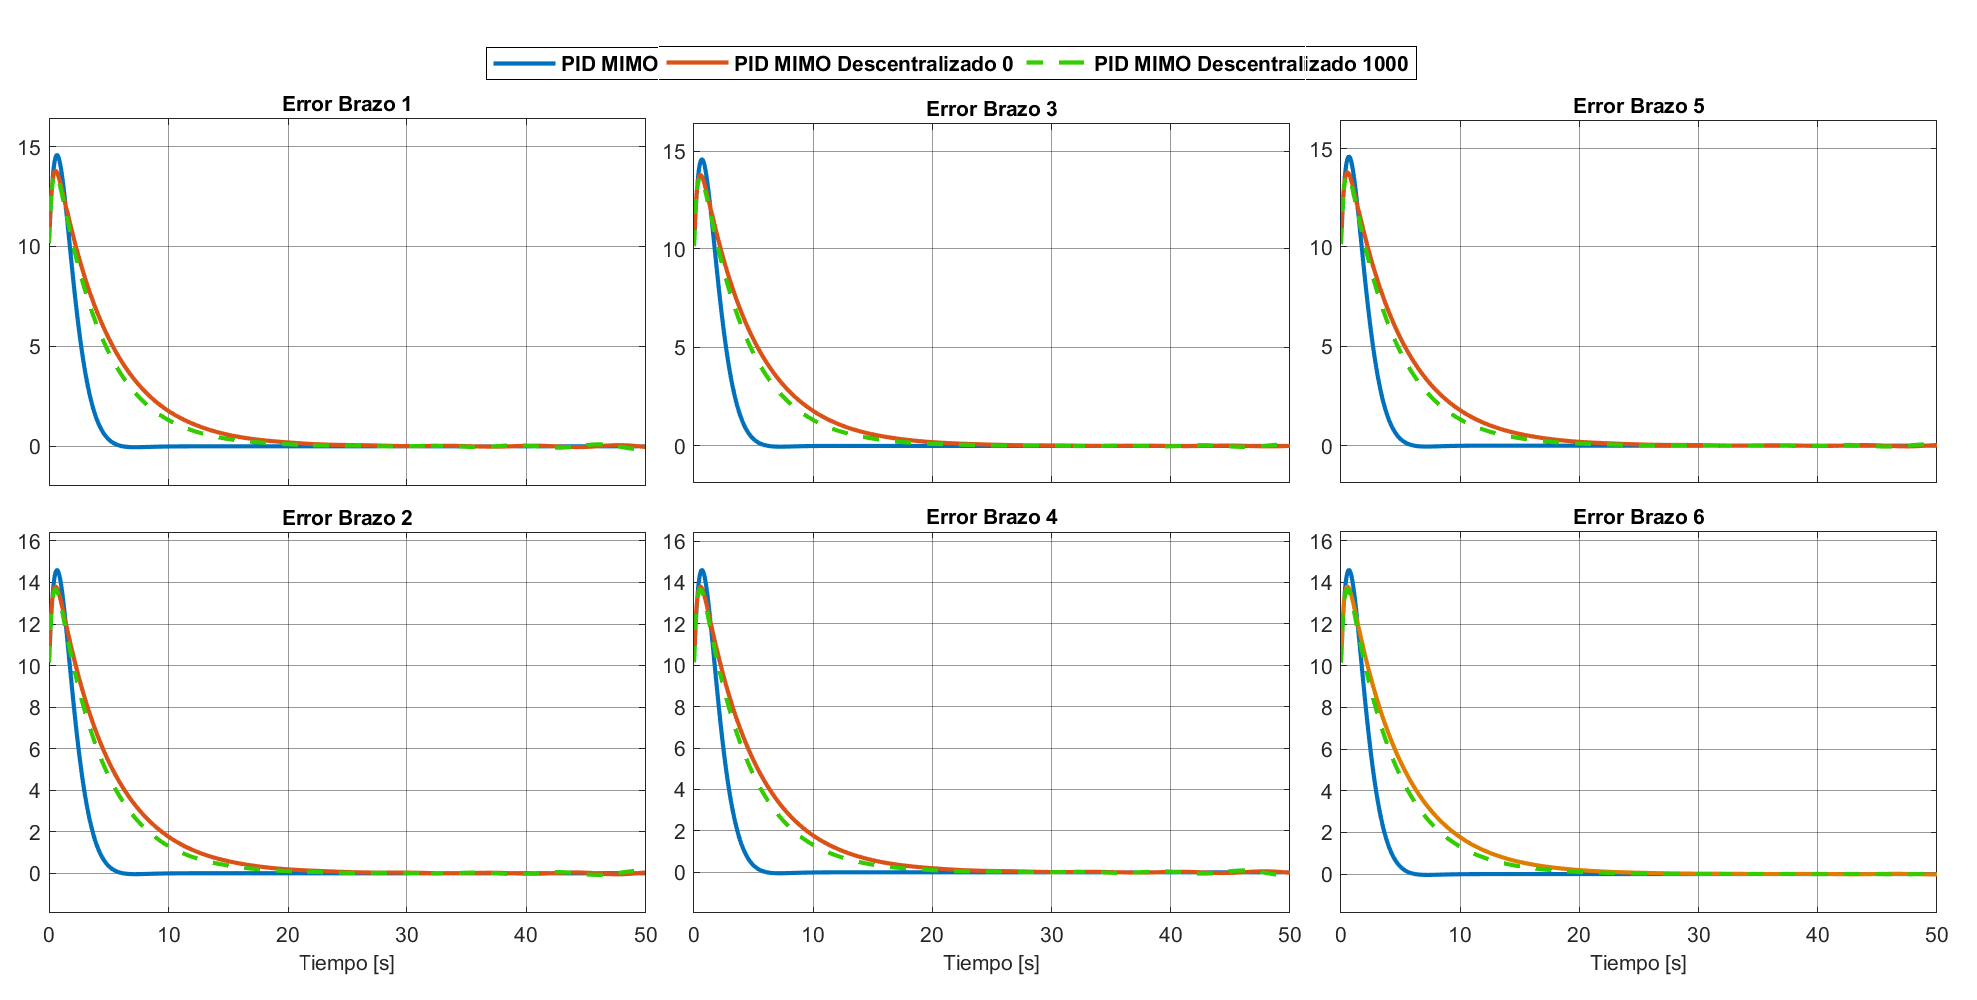
\includegraphics[width=1\columnwidth]{Results/mimoPID_escalon/CASO_1_error_escalon.eps}
    \caption{CASO 1 Error de seguimiento (cm), referencia escalón.}
    \label{fig:result_mimoPID_escalon_error1}
\end{figure}
\newpage
\begin{figure}[H]
\centering
    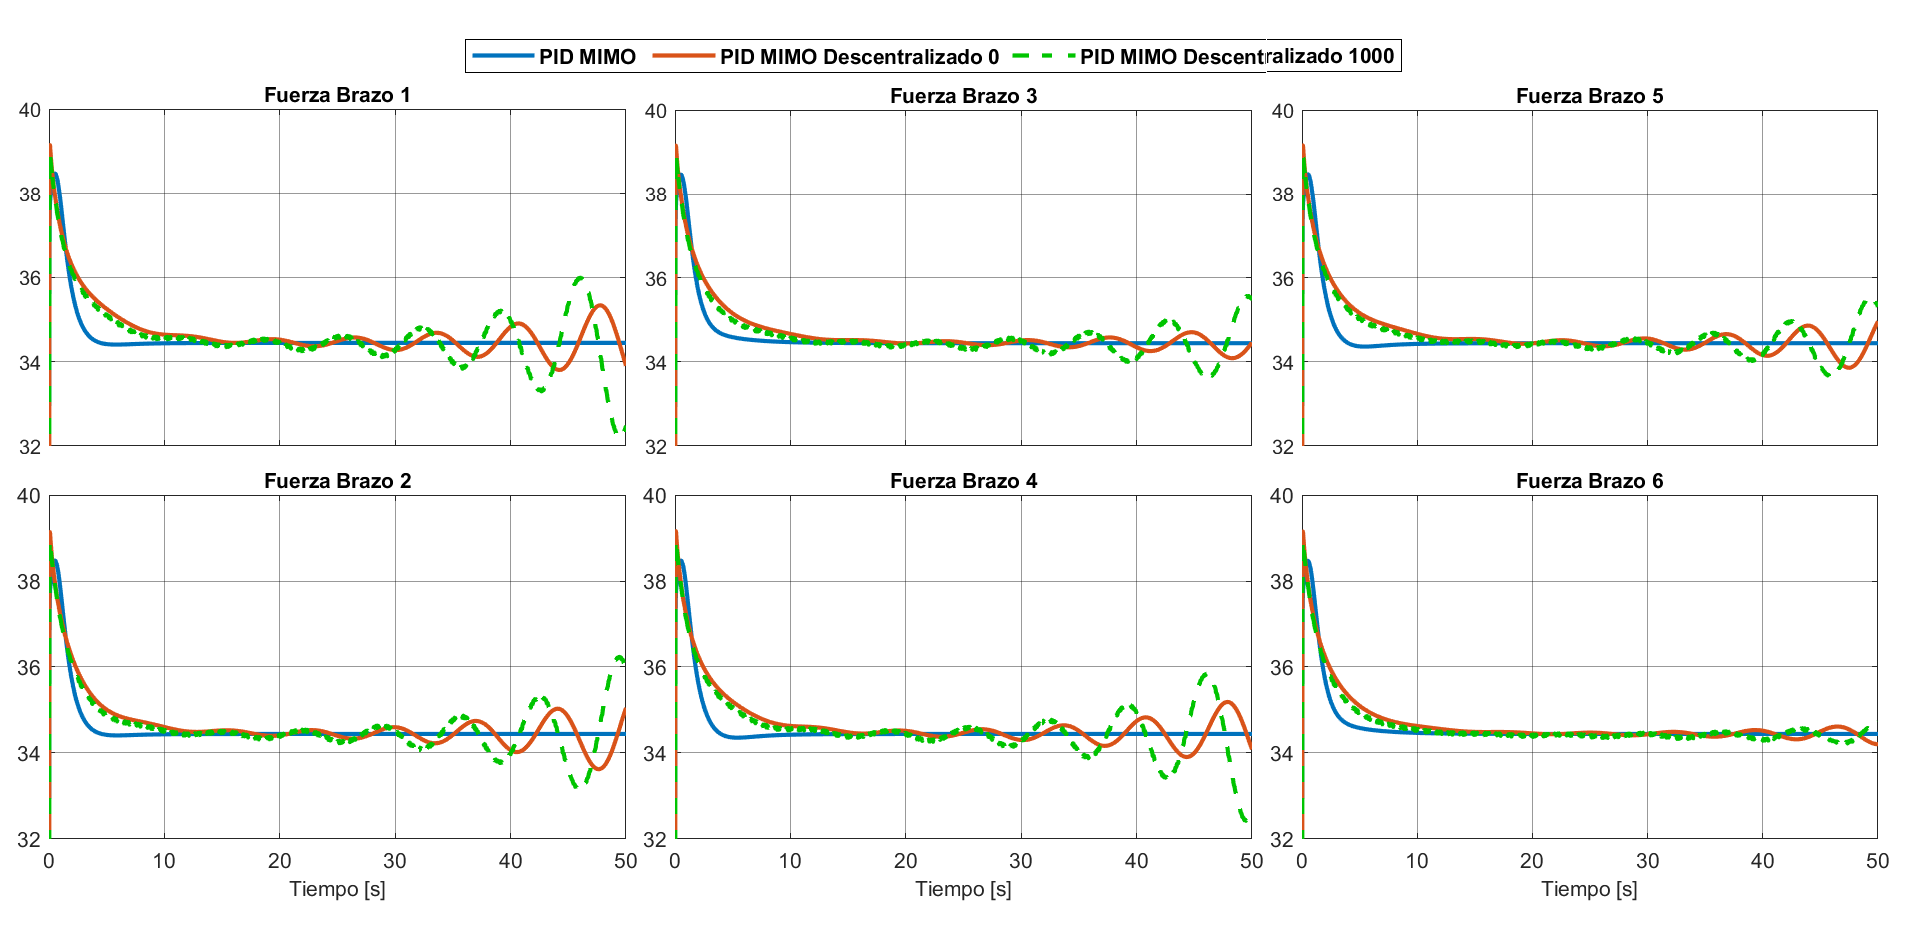
\includegraphics[width=1\columnwidth]{Results/mimoPID_escalon/CASO_1_fuerza_escalon.eps}
    \caption{CASO 1 Fuerza de actuación (N), referencia escalón.}
    \label{fig:result_mimoPID_escalon_fuerza1}
\end{figure}

Para el caso 2, el cambio de las matrices $Q$ y $R$ se traduce en una respuesta más rápida del control, disminuyendo considerablemente el transciente del error y de la fuerza. En las Figuras \ref{fig:result_mimoPID_escalon_error2} y \ref{fig:result_mimoPID_escalon_fuerza2} se muestra el error de seguimiento y la fuerza aplicada respectivamente en cada brazo de la plataforma Stewart. Los 3 tipos de controladores son capaces de estabilizar la plataforma, garantizando un error cero en estado estacionario. 

\begin{figure}[H]
\centering
    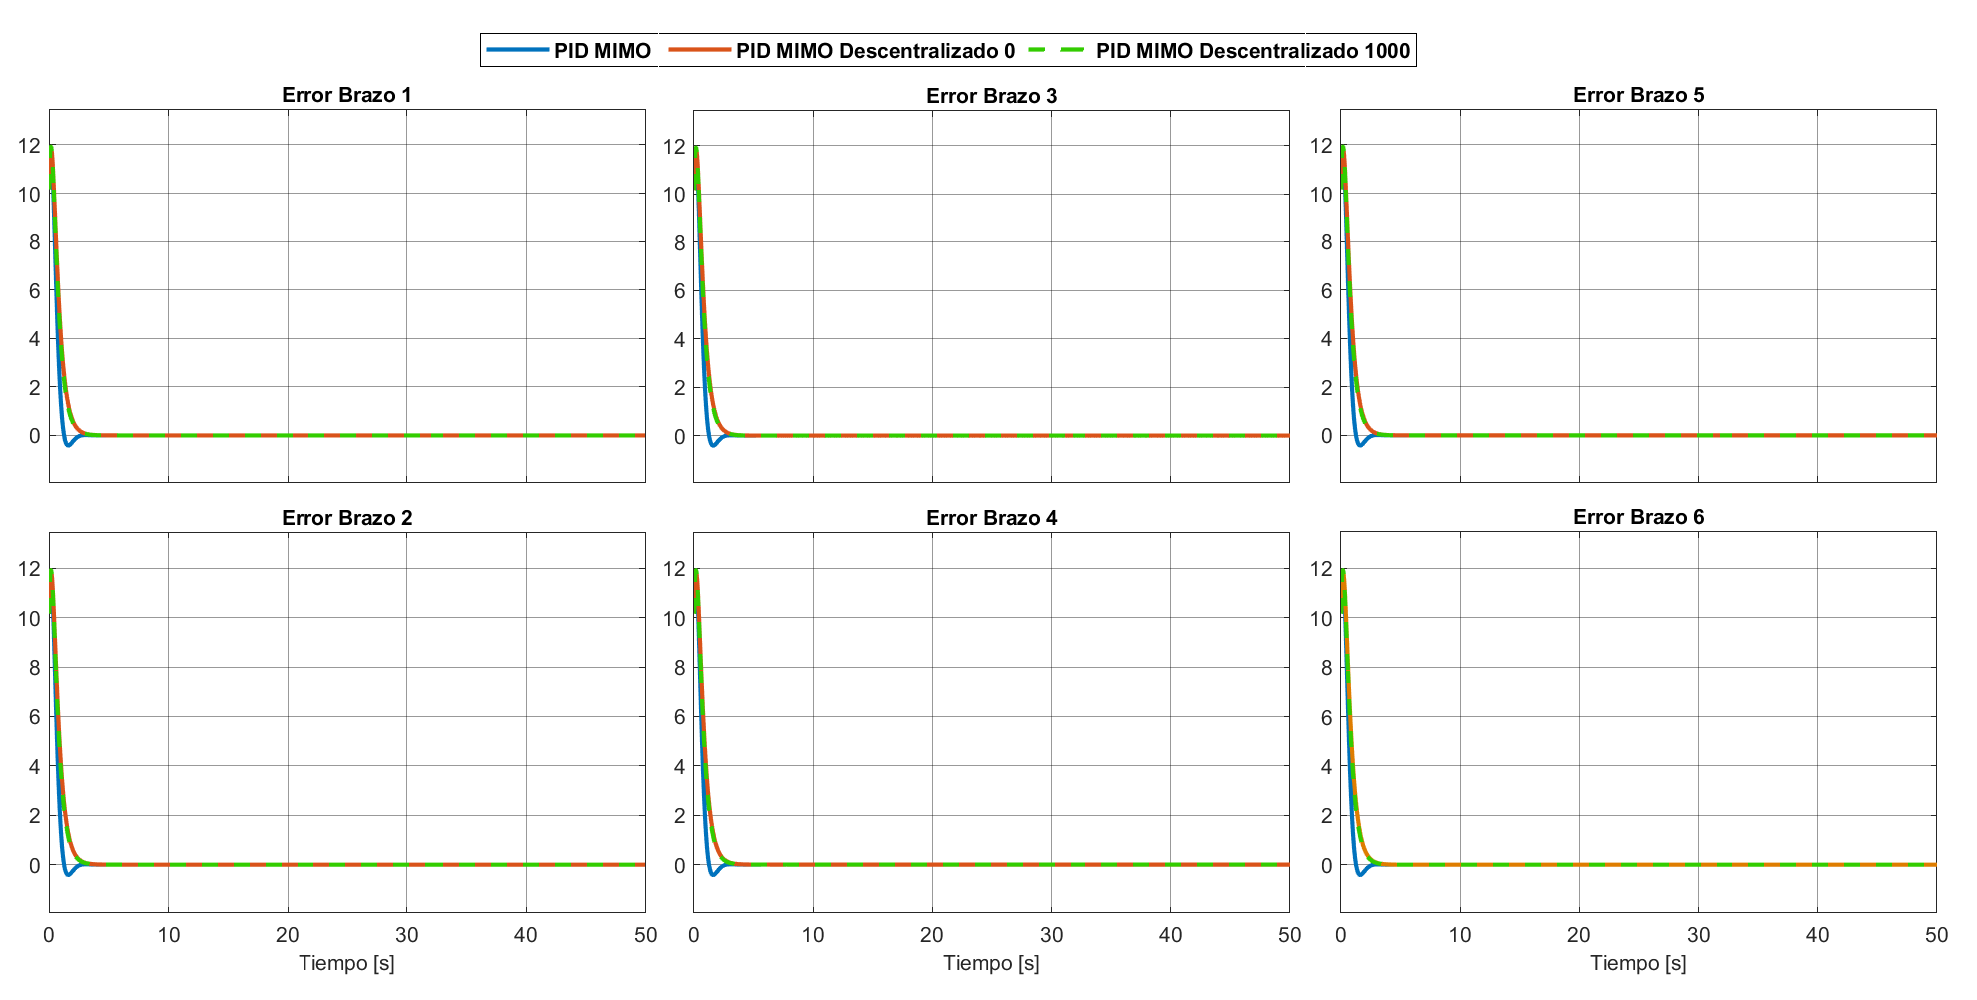
\includegraphics[width=1\columnwidth]{Results/mimoPID_escalon/CASO_2_error_escalon.eps}
    \caption{CASO 2 Error de seguimiento (cm), referencia escalón.}
    \label{fig:result_mimoPID_escalon_error2}
\end{figure}

\begin{figure}[H]
\centering
    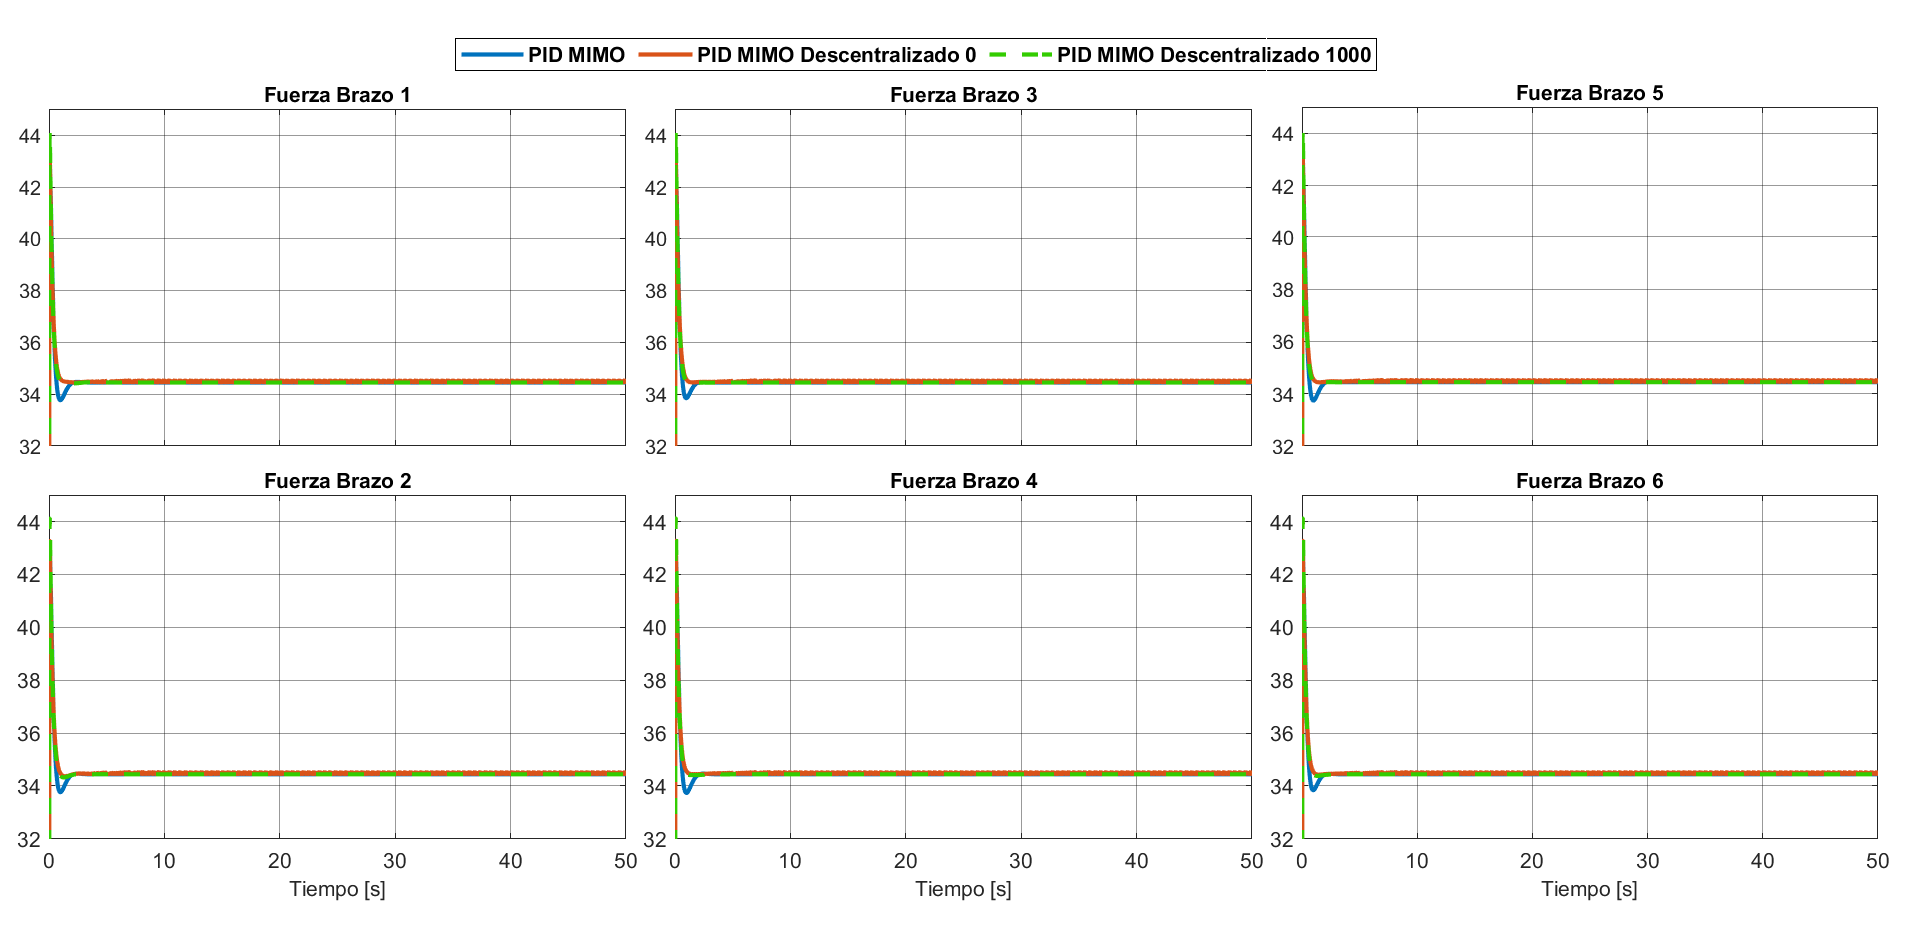
\includegraphics[width=1\columnwidth]{Results/mimoPID_escalon/CASO_2_fuerza_escalon.eps}
    \caption{CASO 2 Fuerza de actuación (N), referencia escalón.}
    \label{fig:result_mimoPID_escalon_fuerza2}
\end{figure}

Finalmente es posible deducir, que los valores de $Q$ y $R$ influyen considerablemente en la estabilidad de la plataforma Stewart, más específicamente en los controladores descentralizados analizados. Para valores de respuesta de control lenta, los controladores descentralizados normal y optimizado no son capaces de estabilizar la planta. Por lo tanto debido a los resultados, el controlador MIMO PID Full logra ser el más completo de todos, ya que posee los mejores índices de desempeño, no presenta desestabilizaciones, y garantiza además error cero en estado estacionario, para señales de referencia de tipo escalón.

%%%%%%%%%%%%%%%%%%%%%%%%%%%%%%%%%%%%%%%%%%%%%%%%
\subsection{Referencia Sinusoidal Nro 1 (caso estable)}

Se establece la señal de referencia para el movimiento de la plataforma superior, compuesta por señales de tipo sinusoidales:
\begin{equation} 
    q_{ref} = \begin{bmatrix}
        0 & 0 & 12+3sin(\pi t) & 0 & 0 & 15sin(\pi t)
    \end{bmatrix}^{\top}
\end{equation}

\begin{remark}
En el modelo Simulink de la simulación se asigna la referencia en grados (se posee un bloque interno de conversor de grados a radianes).
\end{remark}

Para un tiempo de simulación de $T_{sim}=50(s)$ se obtienen los resultados de los índices de desempeño mostrados en la tabla comparativa \ref{tab:indices_mimopid_sinusoidal_nro1}.

\begin{table}[ht]
\centering
\begin{tabular}{c|c|c|c|c|}
\cline{2-5}
    & \textbf{PID MIMO} & $\mathbf{J_{ISE}}$ & $\mathbf{J_{u}}(\cdot10^5)$ & $\mathbf{J_{LQI}}(\cdot10^6)$ \\ \hline
\multicolumn{1}{|c|}{\multirow{3}{*}{Caso 1}} &  Full               & $3455$ & $3.6281$ & $0.3468$ \\ \cline{2-5} 
\multicolumn{1}{|c|}{}                        & Descentralizado 0   & $4230$ & $3.6494$ & $1.1250$ \\ \cline{2-5} 
\multicolumn{1}{|c|}{}                        & Descentralizado 1000& $3959$ & $3.6444$ & $0.9164$ \\ \hline
\multicolumn{1}{|c|}{\multirow{3}{*}{Caso 2}} & Full                & $2584$ & $3.7691$ & $1.3043$ \\ \cline{2-5} 
\multicolumn{1}{|c|}{}                        & Descentralizado 0   & $2465$ & $3.8132$ & $2.7398$ \\ \cline{2-5} 
\multicolumn{1}{|c|}{}                        & Descentralizado 1000& $2416$ & $3.8533$ & $2.5489$ \\ \hline
\end{tabular}
\caption{Desempeño para PID MIMO Full y PID MIMO Descentralizado con $N=0$ y $N=1000$ iteraciones, referencia sinusoidal Nro 1.}
\label{tab:indices_mimopid_sinusoidal_nro1}
\end{table}

De la tabla \ref{tab:indices_mimopid_sinusoidal_nro1} podemos notar los altos valores del índice $J_{ISE}$ para todos los controladores, debido a la incapacidad de los 3 controladores de seguir a la referencia sinusoidal número 1. Debido a esto, es que este índice $J_{ISE}$ no sigue el mismo comportamiento del caso de la referencia escalón. De acá, se aprecia que el controlador MIMO PID Descentralizado 1000 posee mejor rendimiento que su versión descentralizada no optimizada.

Por otro lado para el índice de esfuerzo de control $J_u$, si tomamos como referencia el controlador MIMO PID Full, el controlador MIMO PID Descentralizado 0 presenta un incremento del $0.5\%$ para el Caso 1 y un $1.17\%$ para el Caso 2. El controlador óptimo MIMO Descentralizado 1000 posee un incremento del $0.4\%$ para el Caso 1 y un $2.2\%$ para el Caso 2. Esto nos dice que el controlador MIMO PID Full necesita de un esfuerzo de control menor para controlar el sistema, siendo mejor que las versiones descentralizadas en este ámbito.

Finalmente para el funcional de costo $J_{LQI}$ notamos que el controlador MIMO PID Full minimiza de mejor manera en comparación a sus versiones descentralizadas. Tomando como referencia el controlador MIMO PID Full se puede notar que el controlador MIMO PID Descentralizado 0 posee un incremento del índice $J_{LQI}$ del $224\%$ para el Caso 1 y un $110\%$ para el Caso 2. Para el controlador optimizado MIMO PID Descentralizado 1000 se posee un incremento del $164\%$ para el Caso 1 y un $95\%$ para el Caso 2.

Con estos índices analizados, se podría decir que el controlador MIMO PID Full es la mejor opción en la mayoría de los índices de desempeño para la referencia sinusoidal número 1. Aun así, en el caso 2 se presenta una anomalía donde el controlador optimizado descentralizado 1000 presenta mejor desempeño en el índice $J_{ISE}$ que el controlador MIMO PID Full, que posiblemente sea por la incapacidad de seguir de forma adecuada a la señal sinusoidal número 1. Puede darse el caso de que al cambiar la frecuencia, el MIMO PID Full sea mejor en el índice $J_{ISE}$, pero como se menciono, debido a la incapacidad del diseño de control de seguir a referencias sinusoidales es que da lugar a que se presenten estas anomalías.

En las Figuras \ref{fig:result_mimoPID_sinusoidal_nro1_error1} y \ref{fig:result_mimoPID_sinusoidal_nro1_fuerza1} se muestra el error de seguimiento y la fuerza aplicada respectivamente en cada brazo del sistema para el Caso 1. 

Con los $Q$ y $R$ escogidos para el Caso 1, caracterizándose por establecer una velocidad de control un poco más lenta, podemos notar que las versiones descentralizadas del controlador poseen un transciente más extenso, debido a la falta de sus elementos fuera de la diagonal que aportan en el control del sistema. Por otro lado, debido a la incapacidad de todos los controladores de seguir a la referencia sinusoidal Nro.1, es que se poseen magnitudes elevadas del error en estado estacionario.
    
\begin{figure}[H]
\centering
    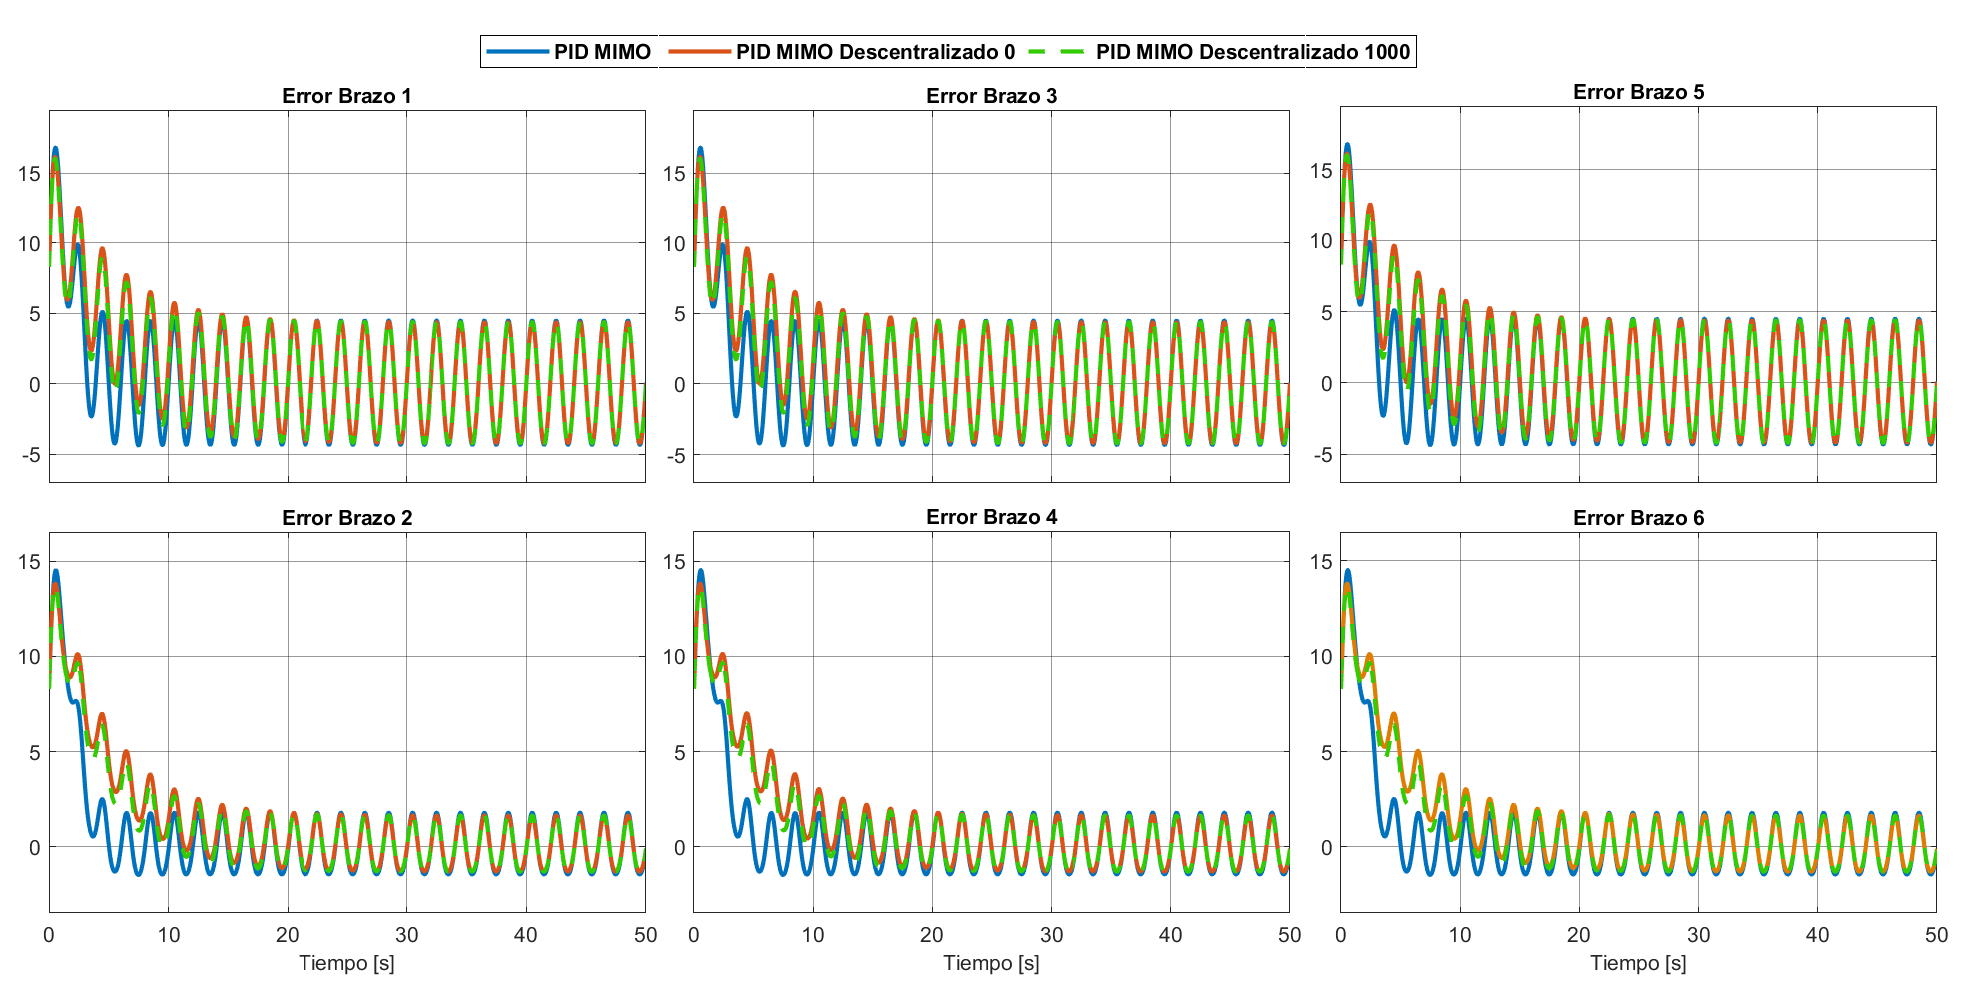
\includegraphics[width=1\columnwidth]{Results/mimoPID_sinusoidal/CASO_1_error_sinusoidal.eps}
    \caption{CASO 1 Error de seguimiento (cm), referencia sinusoidal Nro 1.}
    \label{fig:result_mimoPID_sinusoidal_nro1_error1}
\end{figure}

\begin{figure}[H]
\centering
    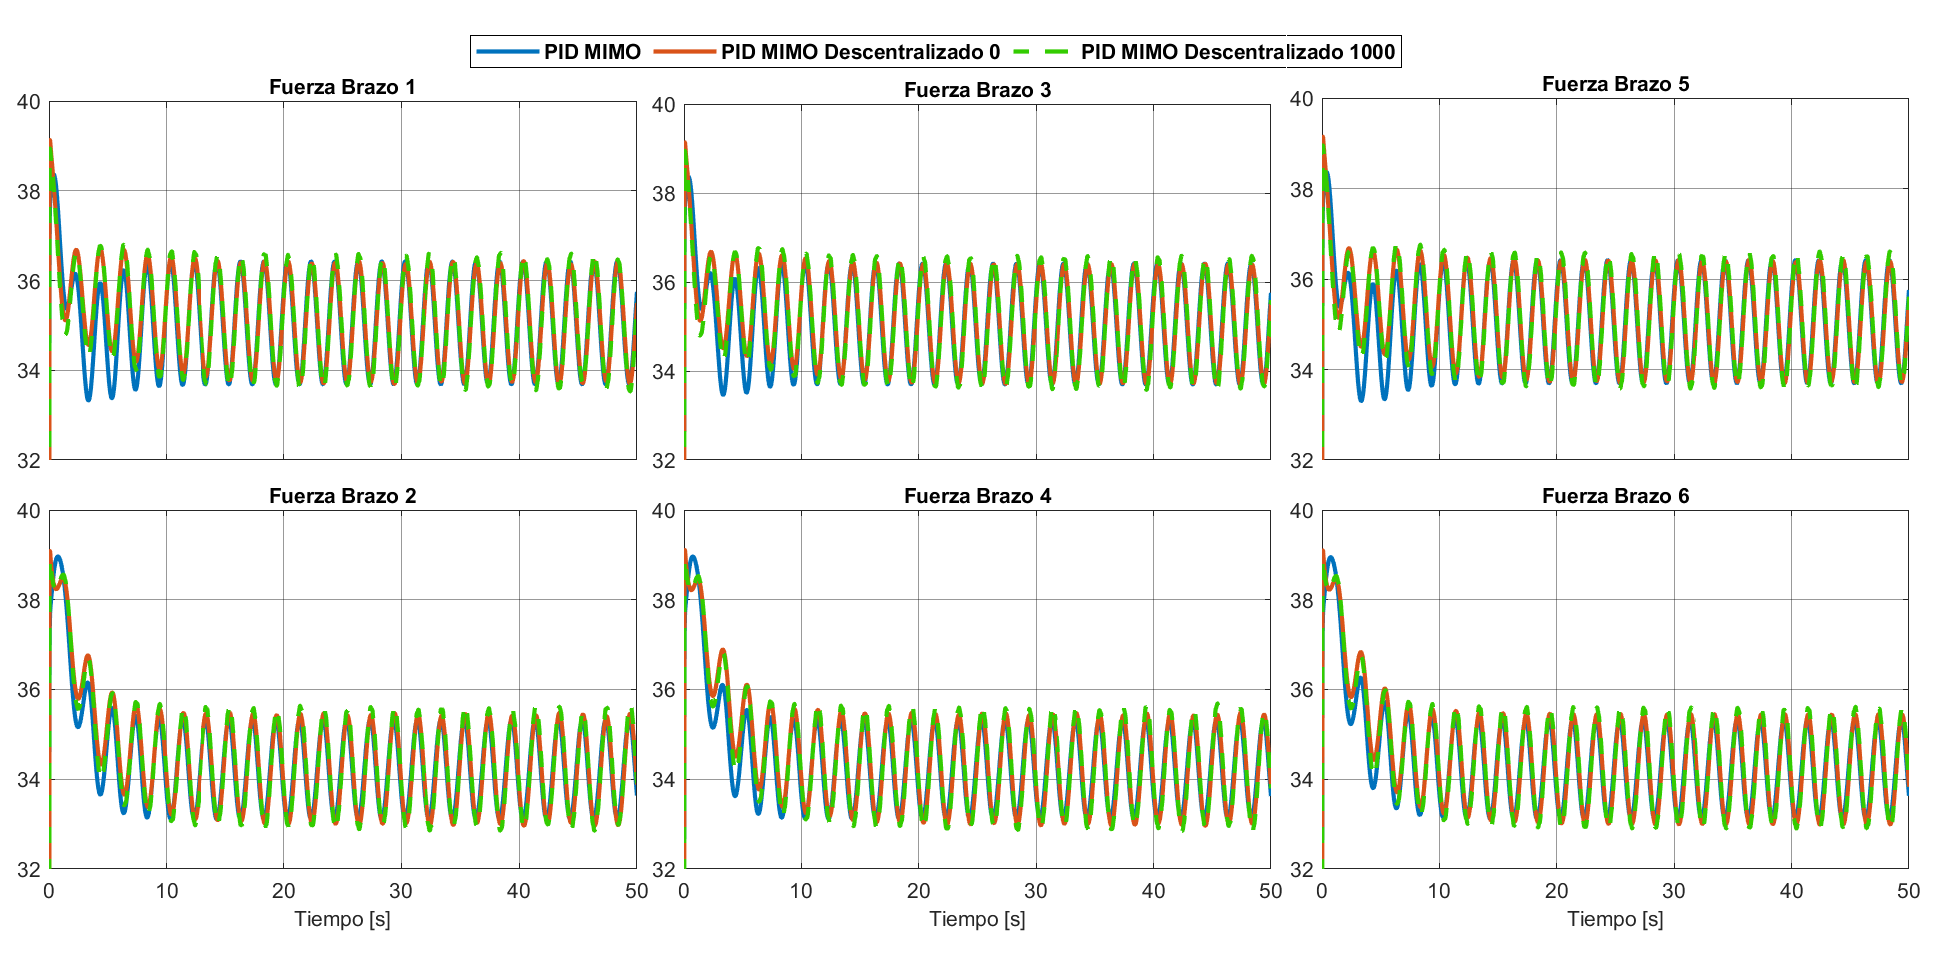
\includegraphics[width=1\columnwidth]{Results/mimoPID_sinusoidal/CASO_1_fuerza_sinusoidal.eps}
    \caption{CASO 1 Fuerza de actuación (N), referencia sinusoidal Nro 1.}
    \label{fig:result_mimoPID_sinusoidal_nro1_fuerza1}
\end{figure}

Para el Caso 2, al cambiar las matrices $Q$ y $R$ logrando una velocidad más rápida del control, seguimos notando altos valores de error y de fuerza aplicada al sistema. En las Figuras \ref{fig:result_mimoPID_sinusoidal_nro1_error2} y \ref{fig:result_mimoPID_sinusoidal_nro1_fuerza2} se muestra el error de seguimiento y la fuerza aplicada respectivamente en cada brazo de la plataforma. 

\begin{figure}[H]
\centering
    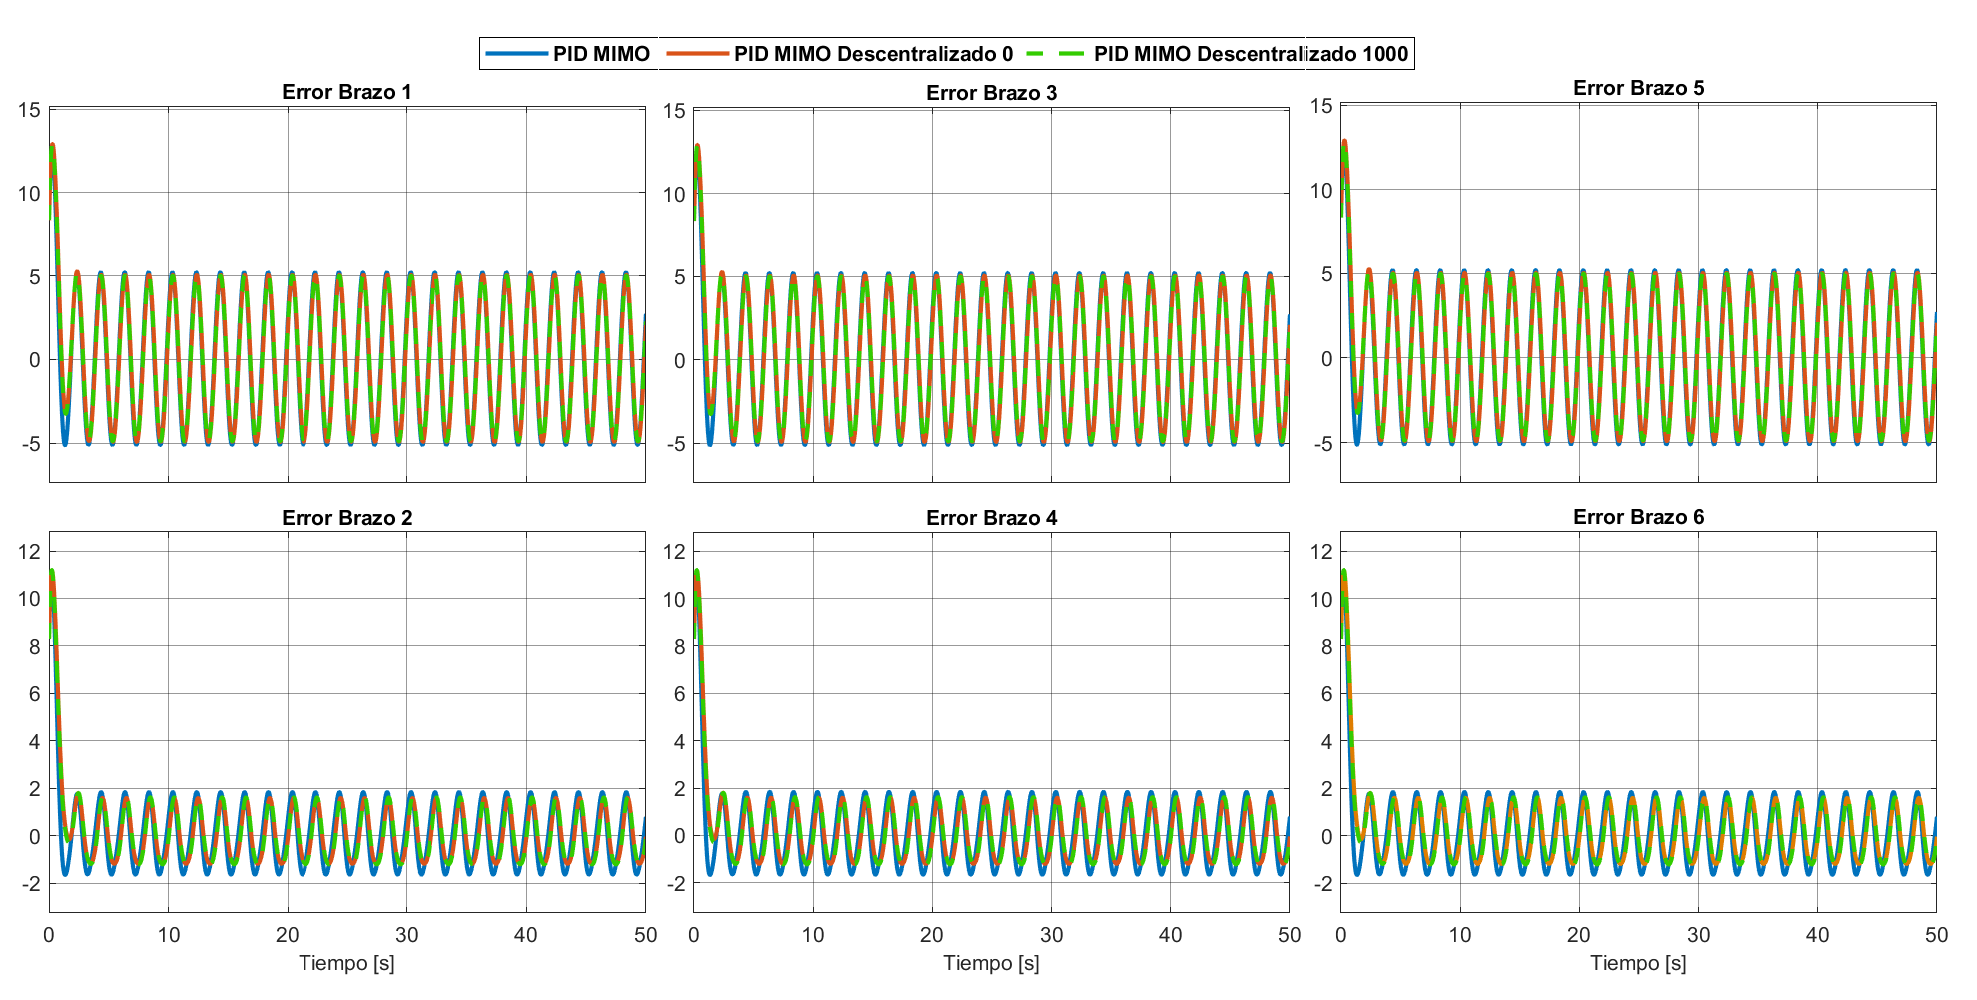
\includegraphics[width=1\columnwidth]{Results/mimoPID_sinusoidal/CASO_2_error_sinusoidal.eps}
    \caption{CASO 2 Error de seguimiento (cm), referencia sinusoidal Nro 1.}
    \label{fig:result_mimoPID_sinusoidal_nro1_error2}
\end{figure}

\begin{figure}[H]
\centering
    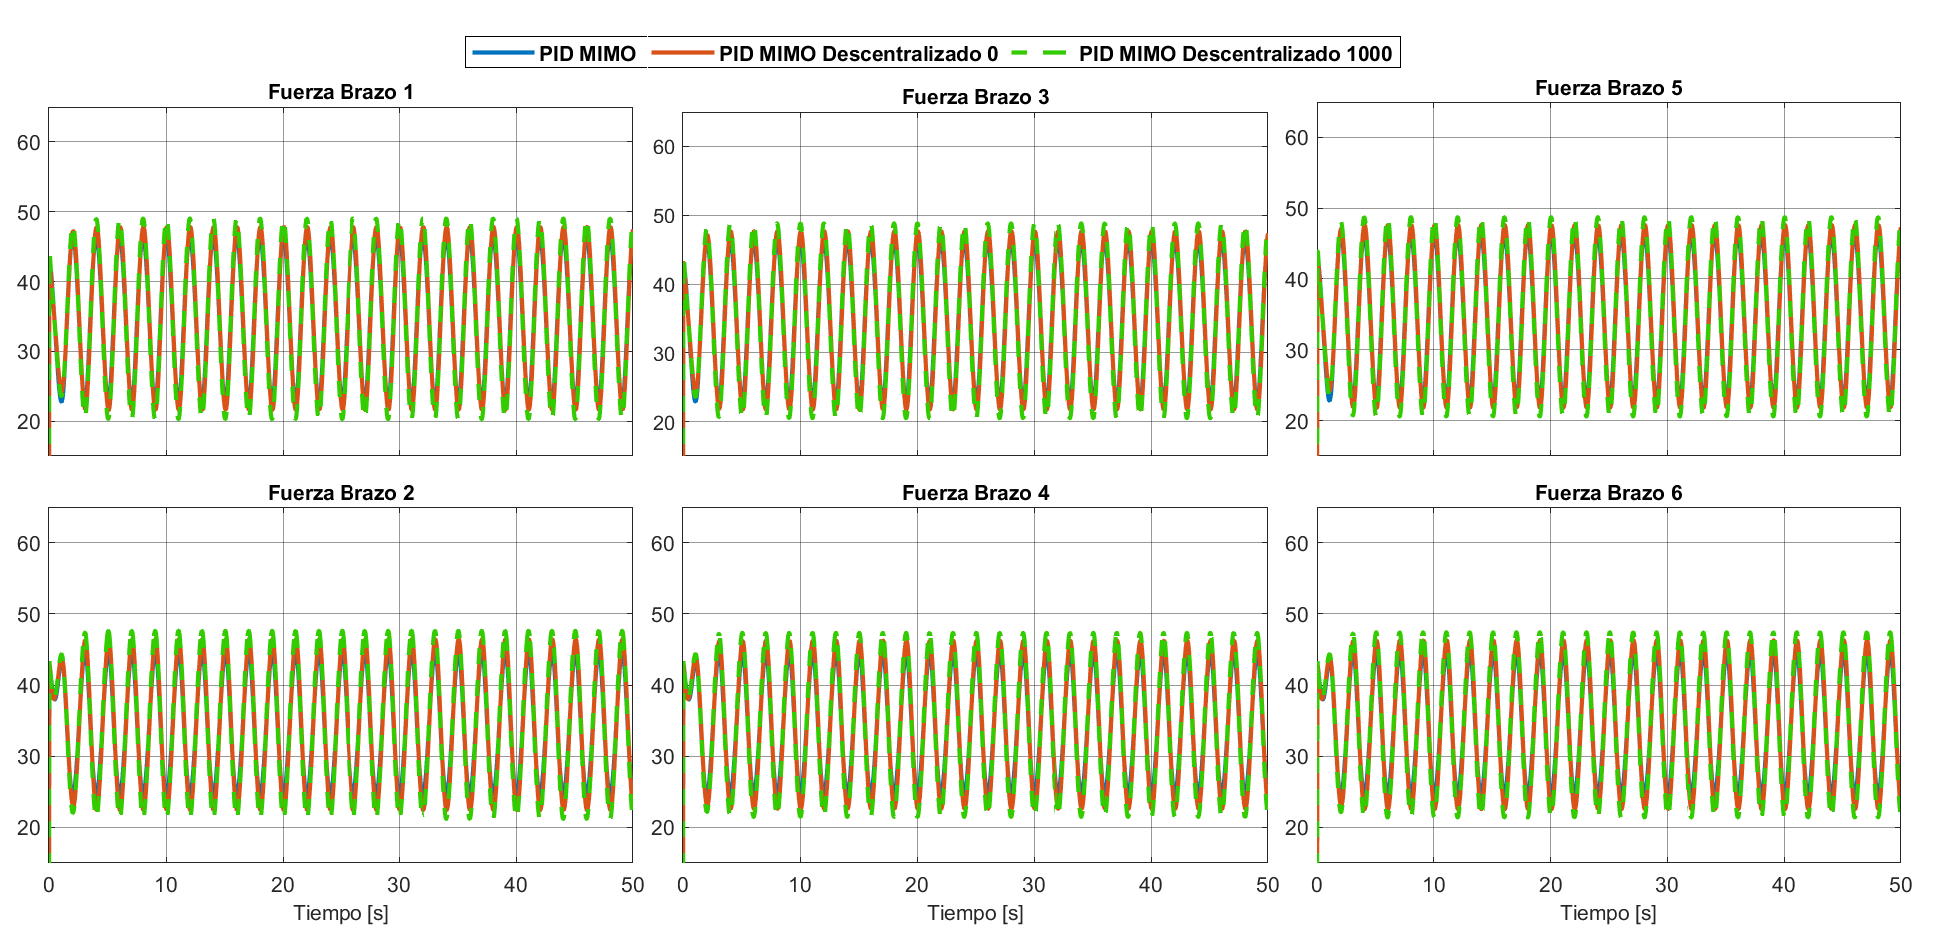
\includegraphics[width=1\columnwidth]{Results/mimoPID_sinusoidal/CASO_2_fuerza_sinusoidal.eps}
    \caption{CASO 2 Fuerza de actuación (N), referencia sinusoidal Nro 1.}
    \label{fig:result_mimoPID_sinusoidal_nro1_fuerza2}
\end{figure}

Por lo tanto, es posible deducir que independiente del valor de $Q$ y $R$ que uno asigne al control, ya sea para aumentar la velocidad de control, no se podrá obtener un seguimiento perfecto a la señal sinusoidal número 1. Esto se evidencia con los altos índices de desempeño analizados y las gráficas de error y de fuerza con sus valores elevados. Se debe notar que el sistema en ningún momento se desestabiliza, es capaz de garantizar cierta estabilidad en el control, pero sin poder garantizar un error de seguimiento cero en estado estacionario.

%%%%%%%%%%%%%%%%%%%%%%%%%%%%%%%%%%%%%%%%%%%%%%%%
\subsection{Referencia Sinusoidal Nro 2 (caso inestable)}

Se establece una segunda señal de referencia de tipo sinusoidal para la plataforma superior, siendo levemente más compleja que la referencia sinusoidal Nro 1, ya que genera un movimiento sinusoidal diferente en cada brazo (diferencias en frecuencia, fase y/o amplitud):

\begin{equation} 
    q_{ref} = \begin{bmatrix}
        0 & 0 & 12+3sin(\pi t) & 10sin(\pi t) & 10sin\left(\pi t - \frac{\pi}{2}\right) & 0
    \end{bmatrix}^{\top}
\end{equation}

\begin{remark}
    En el modelo Simulink de la simulación se asigna la referencia en grados (se posee un bloque interno de conversor de grados a radianes).
\end{remark}

Para un tiempo de simulación de $T_{sim}=50(s)$ se obtienen los resultados de los índices de desempeño mostrados en la tabla comparativa \ref{tab:indices_mimopid_sinusoidal_nro2}.

\begin{table}[ht]
\centering
\begin{tabular}{c|c|c|c|c|}
\cline{2-5}
    & \textbf{PID MIMO} & $\mathbf{J_{ISE}}$ & $\mathbf{J_{u}}(\cdot10^5)$ & $\mathbf{J_{LQI}}(\cdot10^6)$ \\ \hline
\multicolumn{1}{|c|}{\multirow{3}{*}{Caso 1}} &  Full               & $4377$ & $3.6146$ & $0.3794$ \\ \cline{2-5} 
\multicolumn{1}{|c|}{}                        & Descentralizado 0   & $5331$ & $3.6597$ & $1.2664$ \\ \cline{2-5} 
\multicolumn{1}{|c|}{}                        & Descentralizado 1000& $5080$ & $3.7534$ & $1.0319$ \\ \hline
\multicolumn{1}{|c|}{\multirow{3}{*}{Caso 2}} & Full                & $3721$ & $4.4391$ & $1.4834$ \\ \cline{2-5} 
\multicolumn{1}{|c|}{}                        & Descentralizado 0   & $6821$ & $15.362$ & $2.9544$ \\ \cline{2-5} 
\multicolumn{1}{|c|}{}                        & Descentralizado 1000& $3770$ & $9.6146$ & $1.9650$ \\ \hline
\end{tabular}
\caption{Desempeño para PID MIMO Full y PID MIMO Descentralizado con $N=0$ y $N=1000$ iteraciones, referencia sinusoidal Nro 2.}
\label{tab:indices_mimopid_sinusoidal_nro2}
\end{table}

De la tabla \ref{tab:indices_mimopid_sinusoidal_nro2}, al igual que para la referencia de tipo escalón y tipo sinusoidal número 1, el controlador MIMO PID Full posee los mejores índices de desempeño para ambos casos analizados. 

Para el índice del error cuadrático $J_{ISE}$, si tomamos como referencia el controlador MIMO PID Full podemos hacer una comparativa porcentual con sus versiones descentralizadas. El controlador MIMO PID Descentralizado 0 posee un incremento del $J_{ISE}$ del $21.7\%$ para el Caso 1 y un $83.3\%$ para el Caso 2. El controlador optimizado MIMO PID Descentralizado 1000 posee un aumento del $16\%$ en el Caso 1 y un $1.3\%$ en el Caso 2.

Si en el esfuerzo de control $J_u$ tomamos como referencia el controlador MIMO PID Full, notamos que el controlador MIMO PID Descentralizado 0 posee un incremento de $1.2\%$ para el Caso 1 y un $246\%$ para el Caso 2. Para el controlador optimizado MIMO PID Descentralizado 1000 se obtiene un aumento del $3.8\%$ en el Caso 1 y un $116\%$ en el Caso 2, evidenciándose la inestabilidad de las versiones descentralizadas en el Caso 2.

Finalmente al analizar el funcional de costo $J_{LQI}$ la versión MIMO PID Full del controlador es la que mejor minimiza el funcional. Tomando este controlador como referencia, notamos que el controlador MIMO PID Descentralizado 0 posee un incremento del $233\%$ en el Caso 1 y un $99\%$ en el Caso 2. Para el controlador optimizado MIMO PID Descentralizado 1000 se posee un aumento del $171\%$ para el Caso 1 y un $32.4\%$ para el Caso 2.

Por esto, el controlador MIMO PID Full es el mejor al tener menor error cuadrático $J_{ISE}$, un menor esfuerzo de control $J_u$ y un funcional de coste menor $J_{LQI}$. El algoritmo de optimización logra mejorar los índices del controlador descentralizado, pero aun así, no es capaz de igualar el rendimiento del controlador MIMO PID Full con la referencia sinusoidal número 2.

En las Figuras \ref{fig:result_mimoPID_sinusoidal_nro2_error1} y \ref{fig:result_mimoPID_sinusoidal_nro2_fuerza1} correspondientes al Caso 1, se pueden apreciar los errores de seguimiento y la fuerza de la actuación respectivamente de cada brazo de la plataforma Stewart. El controlador MIMO PID es el único de los 3 controladores que no se desestabiliza, sin embargo posee altos valores de error de seguimiento. Por otro lado, los controladores descentralizados además de poseer valores altos de error de seguimiento, son inestables con el sistema, mostrándose una fuerza de actuación descontrolada a partir de los 30 segundos en adelante. 

\begin{figure}[H]
\centering
    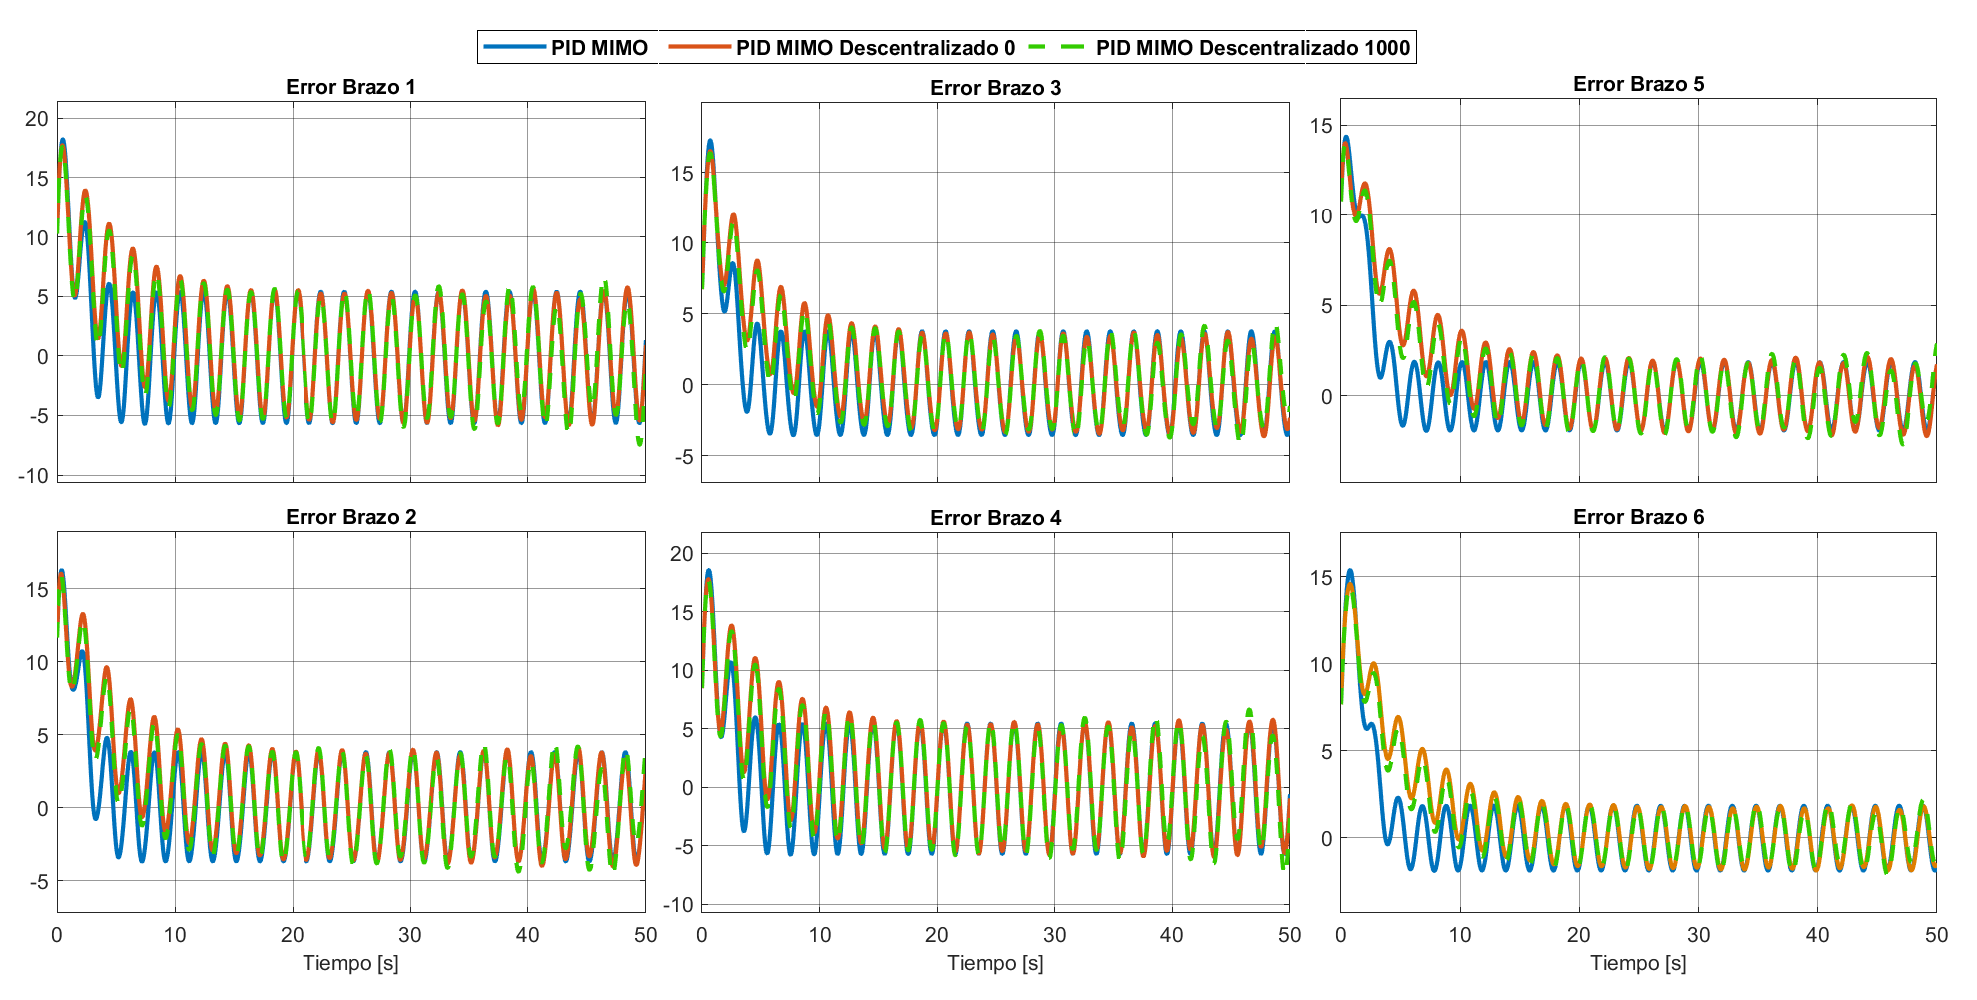
\includegraphics[width=1\columnwidth]{Results/mimoPID_sinusoidal2/CASO_1_error_sinusoidal2.eps}
    \caption{CASO 1 Error de seguimiento (cm), referencia sinusoidal Nro 2.}
    \label{fig:result_mimoPID_sinusoidal_nro2_error1}
\end{figure}
\newpage
\begin{figure}[H]
\centering
    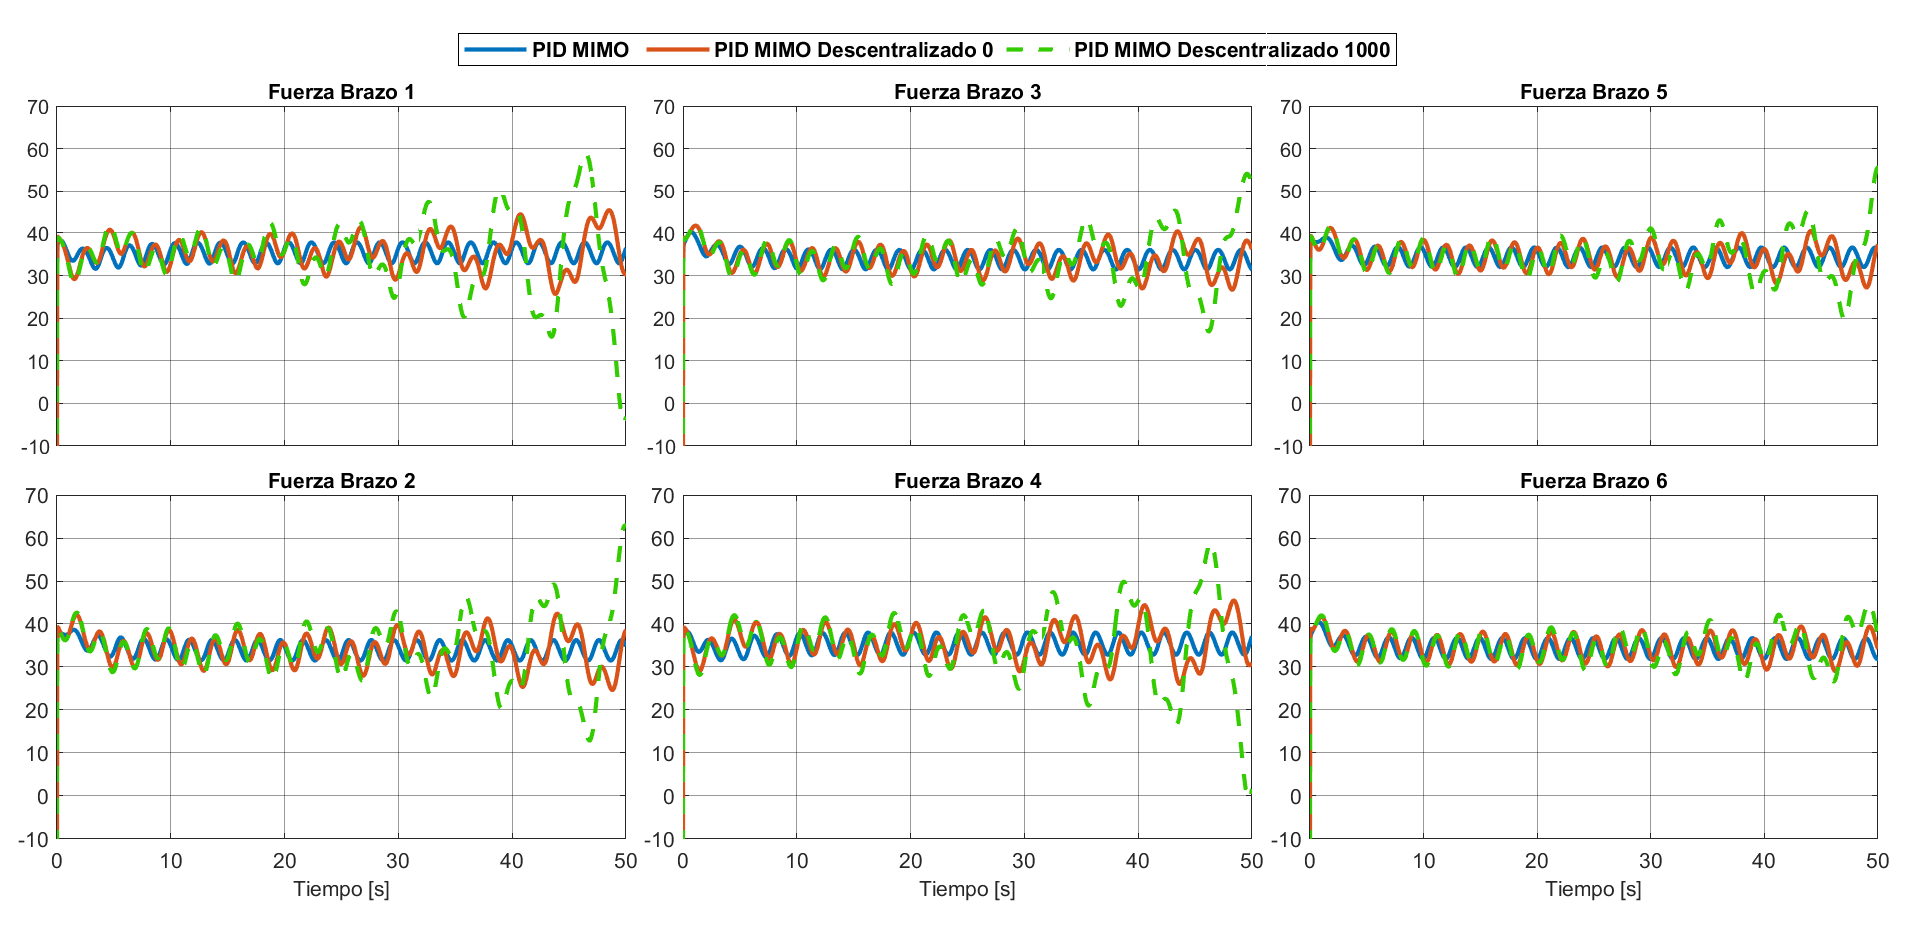
\includegraphics[width=1\columnwidth]{Results/mimoPID_sinusoidal2/CASO_1_fuerza_sinusoidal2.eps}
    \caption{CASO 1 Fuerza de actuación (N), referencia sinusoidal Nro 2.}
    \label{fig:result_mimoPID_sinusoidal_nro2_fuerza1}
\end{figure}


Para el caso 2, el cambio de las matrices $Q$ y $R$ no mejoran la respuesta del sistema ante la señal de referencia sinusoidal número 2. En las Figuras \ref{fig:result_mimoPID_sinusoidal_nro2_error2} y \ref{fig:result_mimoPID_sinusoidal_nro2_fuerza2} se muestran los errores de seguimiento y fuerzas de actuación de los brazos para el Caso 2. Los 3 controladores analizados poseen altos valores de error y de actuación, además de presentar una evidente inestabilidad en todas las gráficas con los controladores descentralizados. 

\begin{figure}[H]
\centering
    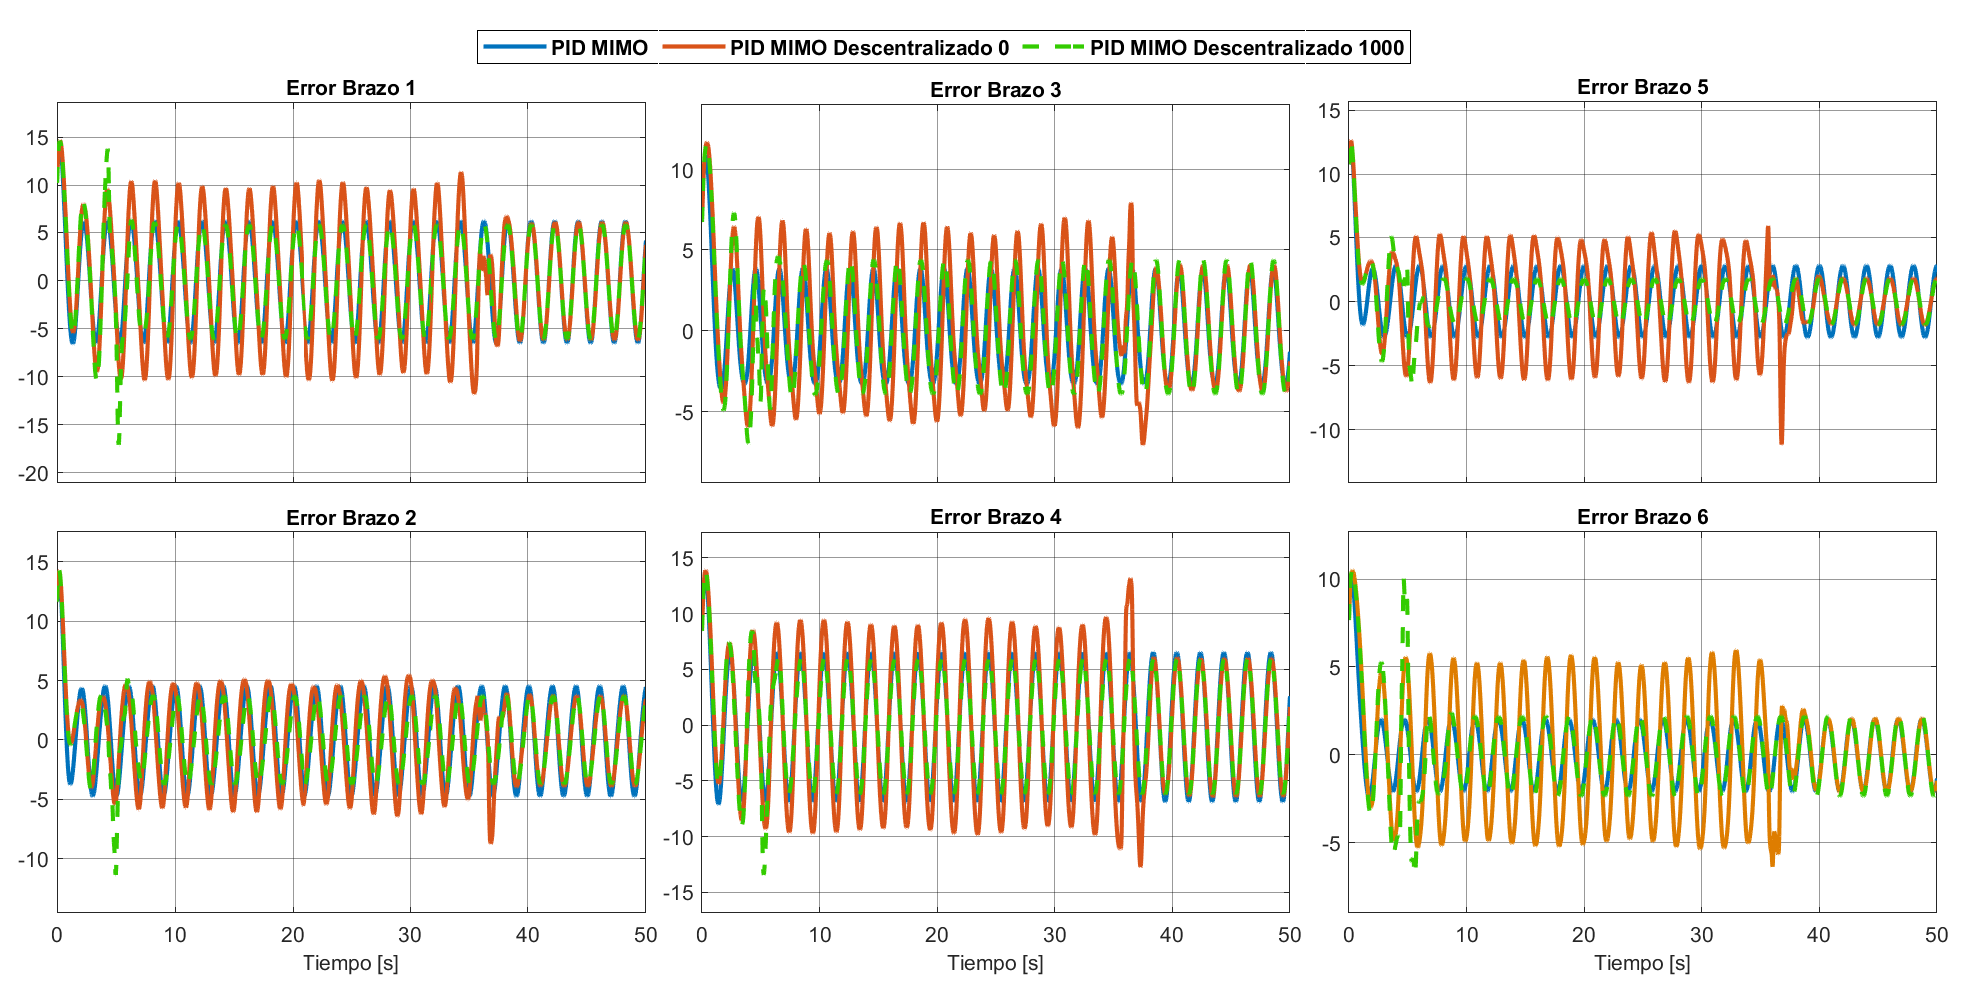
\includegraphics[width=1\columnwidth]{Results/mimoPID_sinusoidal2/CASO_2_error_sinusoidal2.eps}
    \caption{CASO 2 Error de seguimiento (cm), referencia sinusoidal Nro 2.}
    \label{fig:result_mimoPID_sinusoidal_nro2_error2}
\end{figure}

\begin{figure}[H]
\centering
    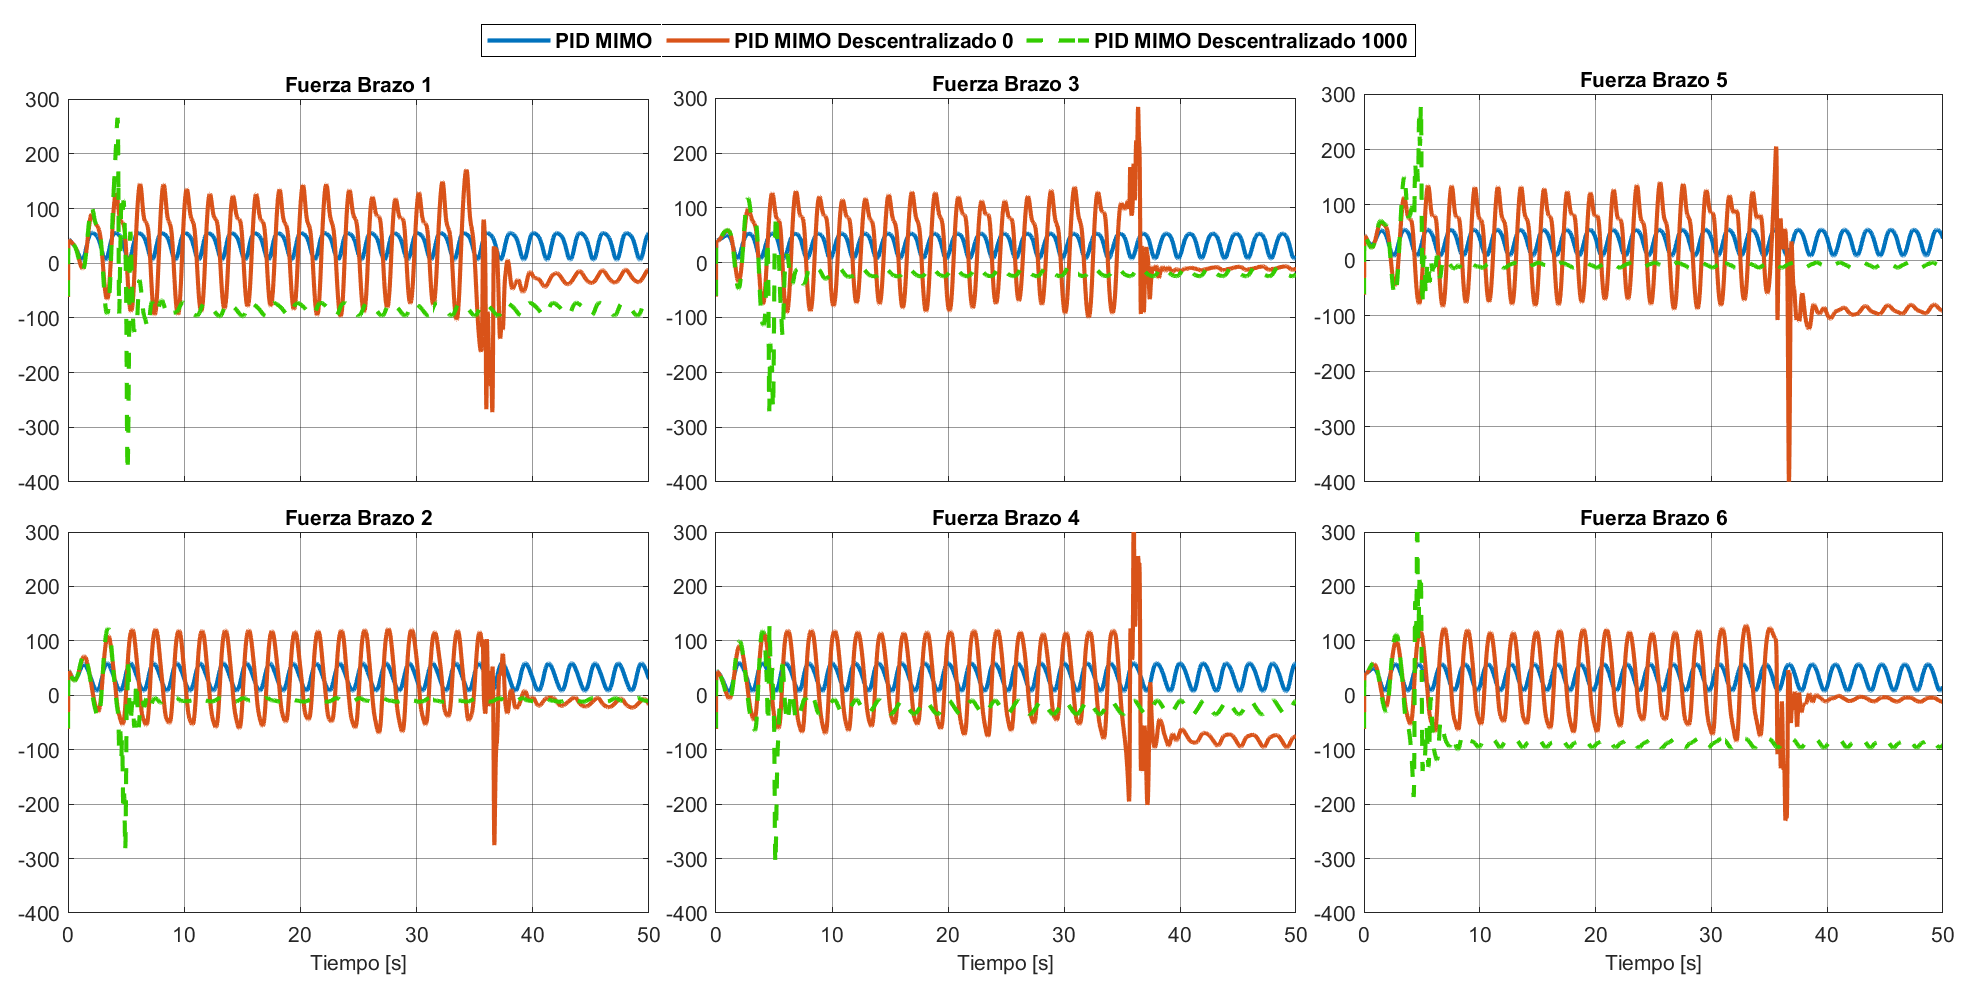
\includegraphics[width=1\columnwidth]{Results/mimoPID_sinusoidal2/CASO_2_fuerza_sinusoidal2.eps}
    \caption{CASO 2 Fuerza de actuación (N), referencia sinusoidal Nro 2.}
    \label{fig:result_mimoPID_sinusoidal_nro2_fuerza2}
\end{figure}

Finalmente es posible deducir, que ante señales de tipo sinusoidales los controladores MIMO PID analizados (full y descentralizados) no son eficientes. Todos ellos presentan altas magnitudes de error de seguimiento, además de inestabilidad por parte de los controladores descentralizados. La ventaja principal del controlador MIMO PID Full con los demás, es que logra garantizar una estabilidad del sistema, además de presentar mejores índices de desempeño en comparación a sus versiones descentralizadas (normal y optimizada), debido a la presencia de los elementos fuera de la diagonal de la matriz de control, pero con el inconveniente de presentar un desempeño claramente deficiente ante referencias sinusoidales\\

Por lo tanto, el diseño de control MIMO PID sintetizado mediante un control LQI no garantiza error de seguimiento cero en estado estacionario para señales de referencia de tipo sinusoidal. Para solucionar esto, en el capítulo \ref{cap:OutputRegulation} siguiente, se diseña un control que garantice un seguimiento eficiente de referencias de señales sinusoidales en estado estacionario.



% =========================== CAPÍTULO 5 ============================ %
\lhead[\thepage]{\thechapter. \rightmark}
\rhead[\leftmark]{\thepage}
\renewcommand{\headrulewidth}{0.5pt}
\lfoot[]{}
\cfoot[]{}
\rfoot[]{}
\renewcommand{\footrulewidth}{0pt}
	
\fancypagestyle{plain}{
	\fancyhead[L]{}
	\fancyhead[C]{}
	\fancyhead[R]{\thepage}
	\fancyfoot[L]{}
	\fancyfoot[C]{}
	\fancyfoot[R]{}
	\renewcommand{\headrulewidth}{0.5pt}
}
	\chapter{OUTPUT REGULATION PARA SEGUIMIENTO A SEÑALES SINUSOIDALES}
\label{cap:OutputRegulation}
\markboth{CAPÍTULO \thechapter. OUTPUT REGULATION}{CAPÍTULO \thechapter. OUTPUT REGULATION}

En este capítulo se resuelve la problemática del seguimiento sinusoidal para la plataforma Stewart. Para esto se desarrolla un nuevo controlador basado en los controladores MIMO PID obtenidos en el capítulo \ref{cap:mimoPID} anterior sintetizados mediante diseño de control LQI. Mediante el principio del modelo interno se obtiene una solución estable para esta problemática. Los resultados del controlador son simulados y comparados mediante tablas bajo distintos índices de desempeño. 

Para modo de simplificación, en el diseño de los controladores con Output Regulation y simulaciones respectivas, la referencia asignada en este capítulo \ref{cap:OutputRegulation} sera con respecto a la posición de los brazos $l(t)$ específicamente. No se considerará el movimiento de la plataforma superior $q_{ref}(t)$ como referencia para este capítulo. 

Se considerarán 2 casos de referencias sinusoidales, la primera referencia de igual señal sinusoidal para todos los brazos de la plataforma (misma amplitud, frecuencia y fase), mientras que la segunda referencia poseerá distintas señales sinusoidales para cada brazo.

\newpage
\section{Diseño control LQR con Output Regulation para referencias sinusoidales de única frecuencia}
\lhead[\thepage]{Sección \thesection. LQR Output Regulation frecuencia única}
\label{sec:LQR_outputRegulation_frec_fija}

Se considera el sistema linealizado \ref{eq:sys_varestados_transf} con la transformación de similaridad de la plataforma Stewart, desarrollado en la sección \ref{sec:linealizacion_stewart} del Capítulo \ref{cap:modeladoStewart}. Recordando las ecuaciones del sistema:

\begin{subequations} \label{eq:sysStewart_outputregulation}
    \begin{align}
        \Dot{\xi}(t) & = A_0 \cdot \xi(t) + B_0 \cdot u(t), \\
        y(t) & = C_0 \cdot \xi(t) + D_0 \cdot u(t)
    \end{align}    
\end{subequations}
con los estados internos
\begin{align} 
    \xi (t) & = \begin{bmatrix}
        l(t)^{\top} & \dot{l}(t)^{\top}
    \end{bmatrix}^{\top} \notag \\
    & = \begin{bmatrix}
        l_1(t) & \hdots & l_6(t) & \dot{l}_1(t) & \hdots & \dot{l}_6(t)
    \end{bmatrix}^{\top}
\end{align}

Como $C_0 = I_{12\times12}$ y $D_0 = 0$ se obtiene como medición directa de la plataforma los estados internos del sistema correspondientes a la posición y velocidad de los brazos. \\

Se define la nueva referencia sinusoidal para el diseño de control LQR con Output Regulation. Esta referencia se caracteriza por modelar la posición de los brazos (no velocidad), además de poseer una frecuencia $\theta$, fase $\phi$ y amplitudes $\Upsilon_{sin}$ $\Upsilon_{step}$ iguales para cada brazo:

\begin{equation}
    l_{ref}(t) = \begin{bmatrix}
        \Upsilon_{sin} sin(\theta t + \phi) + \Upsilon_{step}\\
        \Upsilon_{sin} sin(\theta t + \phi) + \Upsilon_{step}\\
        \Upsilon_{sin} sin(\theta t + \phi) + \Upsilon_{step}\\
        \Upsilon_{sin} sin(\theta t + \phi) + \Upsilon_{step}\\
        \Upsilon_{sin} sin(\theta t + \phi) + \Upsilon_{step}\\
        \Upsilon_{sin} sin(\theta t + \phi) + \Upsilon_{step}\\
    \end{bmatrix}
\end{equation}

Se transforma la referencia de los 6 brazos como sistema independiente exógeno tal como se explica en el problema de Output Regulation de la sección \ref{sec:outputregulation} del Capítulo \ref{cap:Notación y preliminares}. 

Para este caso, el sistema exógeno de la referencia estará formado por 3 estados internos correspondientes a un escalón, una sinusoidal y su derivada, de la forma $v(t)=\begin{bmatrix} step & sin & \frac{d}{dt}(sin) \end{bmatrix}$. Mediante esta representación es posible formar cualquier referencia compuesta por señales escalón y sinusoidal.
\begin{align}
\label{eq:sys_ref_fija}
    \dot{v}(t) & = H_v v(t), \notag \\
    l_{ref}(t) & = C_v v(t)
\end{align}
donde 
\begin{gather}
    \begin{align}
    H_v & = \begin{bmatrix}
        H_{v1} & \hdots & 0 \\
        \vdots & \ddots & \vdots \\ 
        0 & \hdots & H_{v6}
    \end{bmatrix}, 
    \quad \textrm{con } \quad
    H_{vi} = \begin{bmatrix}
        0 & 0 & 0 \\
        0 & 0 & 1 \\
        0 & -\theta^2 & 0
    \end{bmatrix}, \notag \\
    C_v & = \begin{bmatrix}
        C_{v1} & \hdots & 0 \\
        \vdots & \ddots & \vdots \\ 
        0 & \hdots & C_{v6}
    \end{bmatrix},
    \quad \textrm{con } \quad
    C_{vi} = \begin{bmatrix}
        \Upsilon_{step} & \Upsilon_{sin} & 0
    \end{bmatrix},
    \end{align} \\
    v(0) = \begin{bmatrix}
        \begin{bmatrix} 1 & sin(\phi) & \theta cos(\phi) \end{bmatrix} & \hdots & \begin{bmatrix} 1 & sin(\phi) & \theta cos(\phi) \end{bmatrix} 
    \end{bmatrix}_{1\times18}, \quad 
    \textrm{tal que } i = 1,\hdots,6 \notag
\end{gather}

La importancia del sistema exógeno anterior, es que la matriz $H_v$ posee la información de la frecuencia de cada sinusoidal que se desea seguir en cada brazo. 

Una vez desarrollada la referencia deseada, se procede a diseñar el controlador LQR el cual sera la base para el desarrollo del Output Regulation. 

Tal como se define en la sección \ref{sec:lqicontrol} del Capítulo \ref{cap:Notación y preliminares}, se obtiene mediante el Lema \ref{lem1:riccati_infinto} la matriz de realimentación $K_\xi$ del control LQR, encargada de regular los estados internos del sistema \ref{eq:sysStewart_outputregulation} de interés (debe tener incluido el signo negativo propio del control LQR).

Con $K_\xi$ obtenido, se procede a resolver la matriz solución $K_v$ de Output Regulation mediante el Teorema \ref{teo1:OutputRegulation} de la sección \ref{sec:outputregulation} del capítulo \ref{cap:Notación y preliminares}. Se resuelve $X$ y $U$ del sistema de ecuaciones reguladoras (demostrado en Apéndice \ref{appen1}) caracterizado en este caso por: la matriz $H_v$ de los estados de la referencia, la matriz $C_v$ de la referencia deseada y las matrices $A_0, B_0, C_{pos}, D_0$ de la plataforma propiamente tal (como no se tiene ruido en el sistema, entonces $E=0$ y $F=-C_v$ del Teorema \ref{teo1:OutputRegulation}):
\begin{align} \label{eq:OR_equations_fija}
    X H_v = A_0 X + B_0 U \notag \\
    0 = C_{pos} X + D_0 U - C_v 
\end{align}

\begin{remark}
Como se esta regulando unicamente posición de brazos en la referencia, se debe utilizar en las ecuaciones la matriz $C_{pos}=\begin{bmatrix}I_{6\times6} & 0_{6\times6}\end{bmatrix}$ en vez de $C_0$ de la plataforma, para así regular solo posición sin agregar la medición de velocidad disponible.
\end{remark}

Con $X$ y $U$ obtenidos, se despeja $K_v$ desde la igualdad $K_v = U - K_\xi X$.

Finalmente, se obtiene la ley de control final utilizada para el control LQR con Output Regulation de la plataforma Stewart, constituida por una matriz de realimentación $K_\xi$ de los estados internos de la plataforma, junto con una matriz feedforward $K_v$ de los estados de la referencia deseada:

\begin{equation} \label{eq:OR_law_control_fija}
    u(t) = K_\xi \xi(t) + K_v v(t)
\end{equation}






\section{Diseño control LQR con Output Regulation para referencias sinusoidales de distinta amplitud, frecuencia y fase}
\lhead[\thepage]{Sección \thesection. LQR Output Regulation frecuencia variada}

Considerando el mismo sistema linealizado \ref{eq:sysStewart_outputregulation} de la plataforma Stewart, se redefine la referencia deseada diferenciando en amplitud, frecuencia y fase entre cada trayectoria:

\begin{equation}
    l_{ref}(t) = \begin{bmatrix}
        \Upsilon_{sin1} sin(\theta_1 t + \phi_1) + \Upsilon_{step1}\\
        \Upsilon_{sin2} sin(\theta_2 t + \phi_2) + \Upsilon_{step2}\\
        \Upsilon_{sin3} sin(\theta_3 t + \phi_3) + \Upsilon_{step3}\\
        \Upsilon_{sin4} sin(\theta_4 t + \phi_4) + \Upsilon_{step4}\\
        \Upsilon_{sin5} sin(\theta_5 t + \phi_5) + \Upsilon_{step5}\\
        \Upsilon_{sin6} sin(\theta_6 t + \phi_6) + \Upsilon_{step6}\\
    \end{bmatrix}
\end{equation}

Se define el nuevo sistema exógeno, que posee una diferenciación de frecuencia, amplitud y fase a cada trayectoria deseada de cada brazo. 

\begin{align}
\label{eq:sys_ref_variable}
    \dot{v}(t) & = H_v v(t), \notag \\
    l_{ref}(t) & = C_v v(t)
\end{align}
donde 
\begin{gather}
    \begin{align}
    H_v & = \begin{bmatrix}
        H_{v1} & \hdots & 0 \\
        \vdots & \ddots & \vdots \\ 
        0 & \hdots & H_{v6}
    \end{bmatrix}, 
    \quad \textrm{con } \quad
    H_{vi} = \begin{bmatrix}
        0 & 0 & 0 \\
        0 & 0 & 1 \\
        0 & -\theta_i^2 & 0
    \end{bmatrix}, \notag \\
    C_v & = \begin{bmatrix}
        C_{v1} & \hdots & 0 \\
        \vdots & \ddots & \vdots \\ 
        0 & \hdots & C_{v6}
    \end{bmatrix},
    \quad \textrm{con } \quad
    C_{vi} = \begin{bmatrix}
        \Upsilon_{step\textrm{ }i} & \Upsilon_{sin\textrm{ }i} & 0
    \end{bmatrix}, 
    \end{align} \\
    v(0) = \begin{bmatrix}
        \begin{bmatrix} 1 & sin(\phi_1) & \theta_1 cos(\phi_1) \end{bmatrix} & \hdots & \begin{bmatrix} 1 & sin(\phi_6) & \theta_6 cos(\phi_6) \end{bmatrix} 
    \end{bmatrix}, \quad
    \textrm{tal que } i = 1,\hdots,6 \notag
\end{gather}

Después de redefinir la referencia, con las matrices del sistema lineal \ref{eq:sysStewart_outputregulation} se obtiene la matriz de realimentación LQR denominada $K_\xi$ mediante el Lema \ref{lem1:riccati_infinto}, que en este caso es igual a la sección anterior (con signo negativo incluido del control LQR).

Con esta matriz $K_\xi$, se resuelve el mismo sistema de ecuaciones \ref{eq:OR_equations_fija} para $X$ y $U$ (Teorema \ref{teo1:OutputRegulation}), con la nueva matriz de referencia $H_v$ que incluye diferenciación en frecuencia y las matrices del sistema lineal junto a $C_{pos}$ para medir solo posición de la planta. 

Con $X$ y $U$ obtenidos se despeja $K_v$ desde la igualdad $K_v = U - K_\xi X$.

Finalmente se obtiene la misma ley de control \ref{eq:OR_law_control_fija} LQR con Output Regulation para referencias sinusoidales de distintas frecuencias, con $K_\xi$ la matriz estabilizante de los estados internos de la planta y $K_v$ la matriz feedforward de los estados de la referencia. 


%###############################################
%###############################################
%###############################################
\section{Resultados de simulación control LQR con Output Regulation}
\lhead[\thepage]{Sección \thesection. Resultados de simulación LQR con Output Regulation}

Para el control LQR con Output Regulation se utiliza el esquema de control mostrado en la Figura \ref{fig:lqr_OR_stewart_scheme}. Se puede apreciar claramente la matriz de realimentación $K_\xi$ encargada de regular los estados internos del sistema, junto a la matriz feedforward $K_v$ para el seguimiento a la referencia.

\begin{figure}[ht]
\centering
    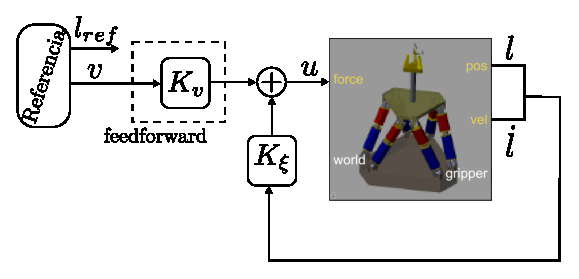
\includegraphics[width=0.7\columnwidth]{Figures/Output_Regulation/lqr_OR_stewart_scheme.eps}
    \caption{Esquema de control LQR con Output Regulation para la plataforma Stewart.}
    \label{fig:lqr_OR_stewart_scheme}
\end{figure}


Se utilizan las matrices $A_0, B_0, C_0, D_0$ del sistema lineal \ref{eq:sysStewart_outputregulation} de la plataforma Stewart.

Con las matrices del sistema lineal, se obtiene la matriz de realimentación $K_\xi$ (con signo negativo incluido) de los estados internos del sistema mediante el Lema \ref{lem1:riccati_infinto}:

\begin{equation}
    K_\xi = \scalebox{0.8}{$\begin{bmatrix}
        \textrm{-}13.433 &	6.858 &	2.100 &	\textrm{-}4.205 &	1.542 &	3.748 &	\textrm{-}3.844 &	0.547 &	0.281 &	\textrm{-}0.394 &	0.120 &	0.087 \\
        6.865 &	\textrm{-}13.400 &	3.743 &	1.520 &	\textrm{-}4.198 &	2.080 &	0.545 &	\textrm{-}3.842 &	0.088 &	0.118 &	\textrm{-}0.393 &	0.280 \\
        1.518 &	3.788 &	\textrm{-}13.476 &	6.865 &	2.098 &	\textrm{-}4.200 &	0.119 &	0.088 &	\textrm{-}3.845 &	0.547 &	0.281 &	\textrm{-}0.395 \\
        \textrm{-}4.176 &	2.117 &	6.856 &	\textrm{-}13.494 &	3.796 &	1.514 &	\textrm{-}0.395 &	0.282 &	0.548 &	\textrm{-}3.846 &	0.089 &	0.119 \\
        2.148 &	\textrm{-}4.157 &	1.495 &	3.787 &	\textrm{-}13.506 &	6.846 &	0.283 &	\textrm{-}0.396 &	0.118 &	0.089 &	\textrm{-}3.847 &	0.548 \\
        3.774 &	1.497 &	\textrm{-}4.192 &	2.101 &	6.875 &	\textrm{-}13.460 &	0.088 &	0.118 &	\textrm{-}0.395 &	0.282 &	0.547 &	\textrm{-}3.845 
    \end{bmatrix}$}
\end{equation}

%--------------------------------------------------
\newpage
\subsection{Referencia sinusoidal Nro.1 frecuencia fija}

Se define la referencia Nro.1 a seguir de cada brazo actuador de la plataforma Stewart, caracterizada por un escalón y sinusoidales de misma amplitud, frecuencia y fase para todos los brazos: 
\begin{equation}
    l_{ref1}(t) = \begin{bmatrix}
        2 sin(\pi t) + 10\\
        2 sin(\pi t) + 10\\
        2 sin(\pi t) + 10\\
        2 sin(\pi t) + 10\\
        2 sin(\pi t) + 10\\
        2 sin(\pi t) + 10\\
    \end{bmatrix}
\end{equation}

Se establecen así los parámetros de la referencia:
\begin{itemize}
    \item amplitud escalón $\Upsilon_{step}=10$.
    \item amplitud sinusoidal $\Upsilon_{sin}=2$, \\
    frecuencia $\theta=\pi$, \\
    fase $\phi=0$.
\end{itemize}

Con los parámetros obtenidos de la referencia se modela su sistema exógeno de \ref{eq:sys_ref_fija}. Con el sistema exógeno de la referencia y los parámetros del sistema \ref{eq:sysStewart_outputregulation} de la plataforma Stewart, se obtiene la matriz feedforward $K_v$ del control para la referencia sinusoidal Nro.1:

\begin{multline}
    K_v = \scalebox{0.75}{$\left[\begin{matrix}
        73.878 &	12.138 &	7.689 &	\textrm{-}29.820 &	\textrm{-}4.249 &	\textrm{-}1.094 &	\textrm{-}10.957 &	\textrm{-}1.612 &	\textrm{-}0.562 &	20.854 &	3.267 &	0.789 \\
        \textrm{-}29.762 &	\textrm{-}4.237 &	\textrm{-}1.091 &	73.682 &	12.099 &	7.685 &	\textrm{-}17.338 &	\textrm{-}3.586 &	\textrm{-}0.175 &	\textrm{-}4.819 &	\textrm{-}0.384 &	\textrm{-}0.237 \\
        \textrm{-}4.844 &	\textrm{-}0.389 &	\textrm{-}0.238 &	\textrm{-}17.338 &	\textrm{-}3.586 &	\textrm{-}0.175 &	73.946 &	12.152 &	7.691 &	\textrm{-}29.876 &	\textrm{-}4.260 &	\textrm{-}1.095 \\
        20.906 &	3.277 &	0.791 &	\textrm{-}11.006 &	\textrm{-}1.621 &	\textrm{-}0.564 &	\textrm{-}29.907 &	\textrm{-}4.266 &	\textrm{-}1.096 &	74.108 &	12.184 &	7.693 \\
        \textrm{-}11.177 &	\textrm{-}1.656 &	\textrm{-}0.567 &	20.881 &	3.272 &	0.792 &	\textrm{-}4.822 &	\textrm{-}0.385 &	\textrm{-}0.236 &	\textrm{-}17.541 &	\textrm{-}3.626 &	\textrm{-}0.179 \\
        \textrm{-}17.347 &	\textrm{-}3.588 &	\textrm{-}0.177 &	\textrm{-}4.740 &	\textrm{-}0.368 &	\textrm{-}0.236 &	20.868 &	3.270 &	0.790 &	\textrm{-}11.063 &	\textrm{-}1.633 &	\textrm{-}0.563 \\
    \end{matrix}\right.$} \\
    \scalebox{0.75}{$\left. \begin{matrix}
        \textrm{-}4.997 &	\textrm{-}0.420 &	\textrm{-}0.240 &	\textrm{-}17.298 &	\textrm{-}3.578 &	\textrm{-}0.174 \\
        20.750 &	3.246 &	0.786 &	\textrm{-}10.849 &	\textrm{-}1.590 &	\textrm{-}0.559 \\
        \textrm{-}10.985 &	\textrm{-}1.617 &	\textrm{-}0.562 &	20.859 &	3.268 &	0.789 \\
        \textrm{-}17.514 &	\textrm{-}3.621 &	\textrm{-}0.177 &	\textrm{-}4.902 &	\textrm{-}0.401 &	\textrm{-}0.237 \\
        74.255 &	12.214 &	7.695 &	\textrm{-}29.912 &	\textrm{-}4.267 &	\textrm{-}1.096 \\
        \textrm{-}29.848 &	\textrm{-}4.255 &	\textrm{-}1.093 &	73.887 &	12.140 &	7.689 \\
    \end{matrix}\right]$}
\end{multline}



\subsubsection{Simulación Sistema Lineal}

En la Figura \ref{fig:lqrOR_lineal_frec_fija} se puede apreciar el error de seguimiento de los brazos actuadores del sistema lineal. Como se puede notar, el efecto del Output Regulation funciona perfectamente al seguir a la referencia sinusoidal de frecuencia única, mostrando un error cero en estado estacionario para el sistema linealizado.

\begin{figure}[H]
\centering
    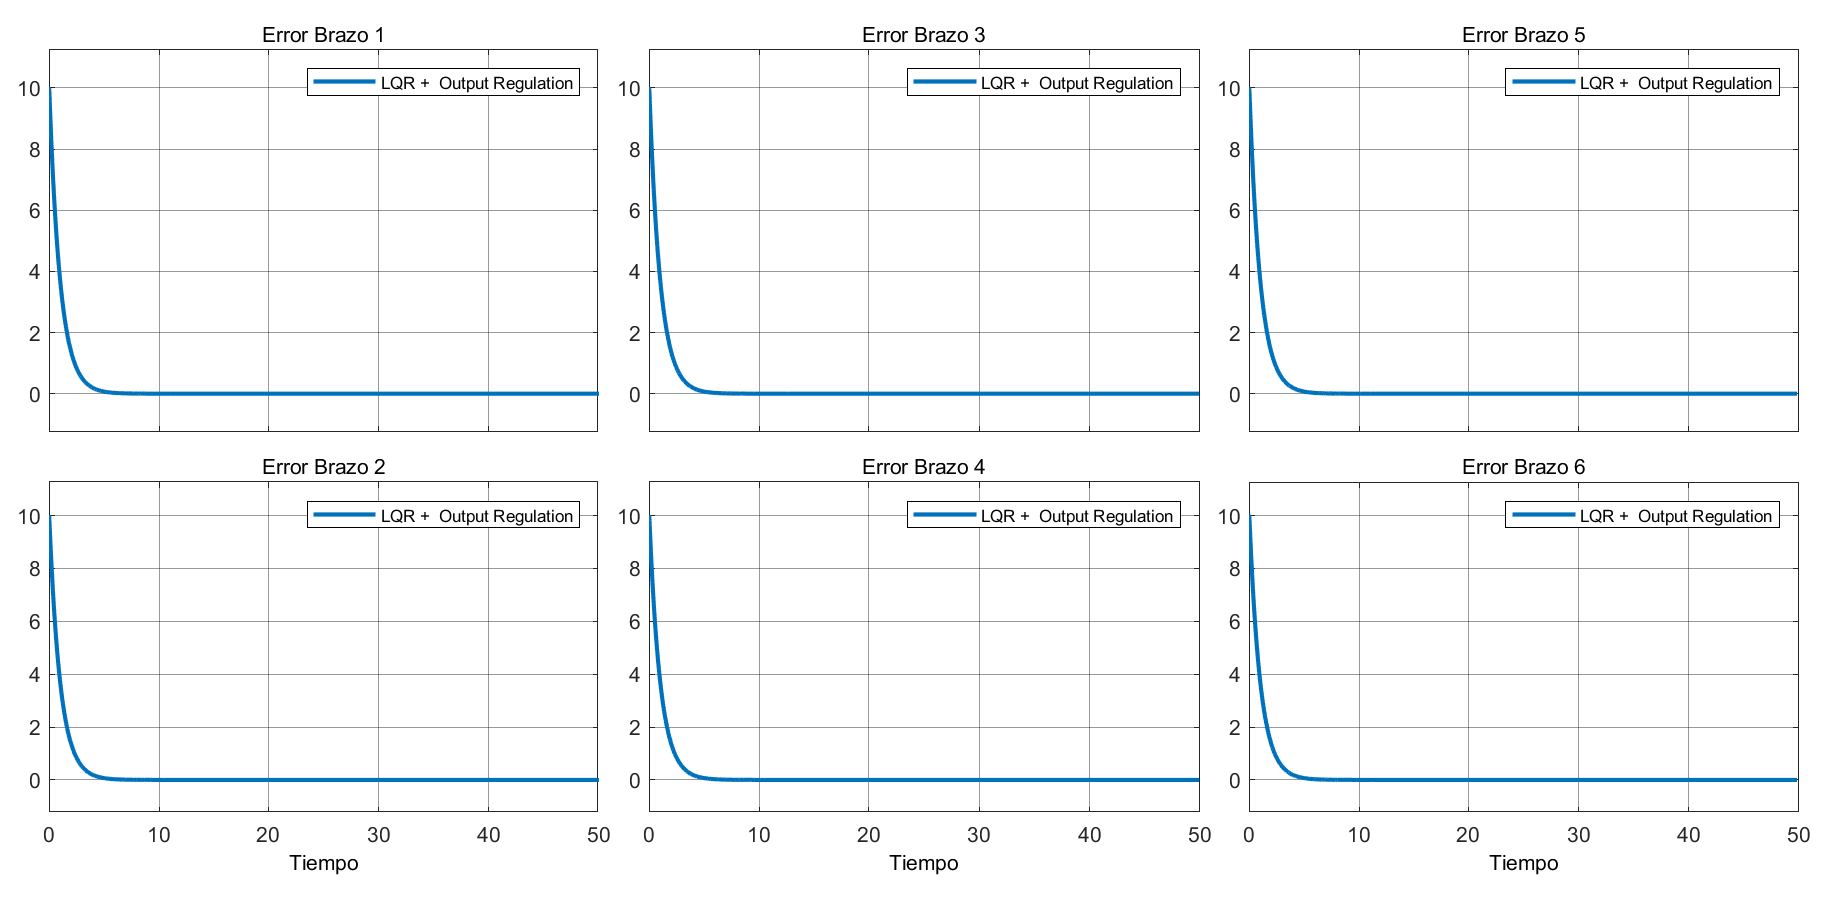
\includegraphics[width=0.9\columnwidth]{Results/lqrOR_frec_fija/lqr_sys_lineal_frec_fija.eps}
    \caption{Error de seguimiento (cm) LQR + Output Regulation sistema lineal, referencia frecuencia fija.}
    \label{fig:lqrOR_lineal_frec_fija}
\end{figure}

\subsubsection{Simulación Sistema No-Lineal}

Se utiliza el sistema no-lineal de la plataforma Stewart para la simulación, mostrando los errores de seguimiento de los brazos en la Figura \ref{fig:lqrOR_real_frec_fija}. Es posible notar que, el seguimiento de la referencia sinusoidal de frecuencia única no se logra adecuadamente. Se ve un error considerable en todos los brazos, que se constituye de un valor constante de aproximadamente $11.8$ sumado a oscilaciones pequeñas pero no despreciables.

Debido al error obtenido, se deberá ajustar el controlador diseñado más adelante.

\begin{figure}[H]
\centering
    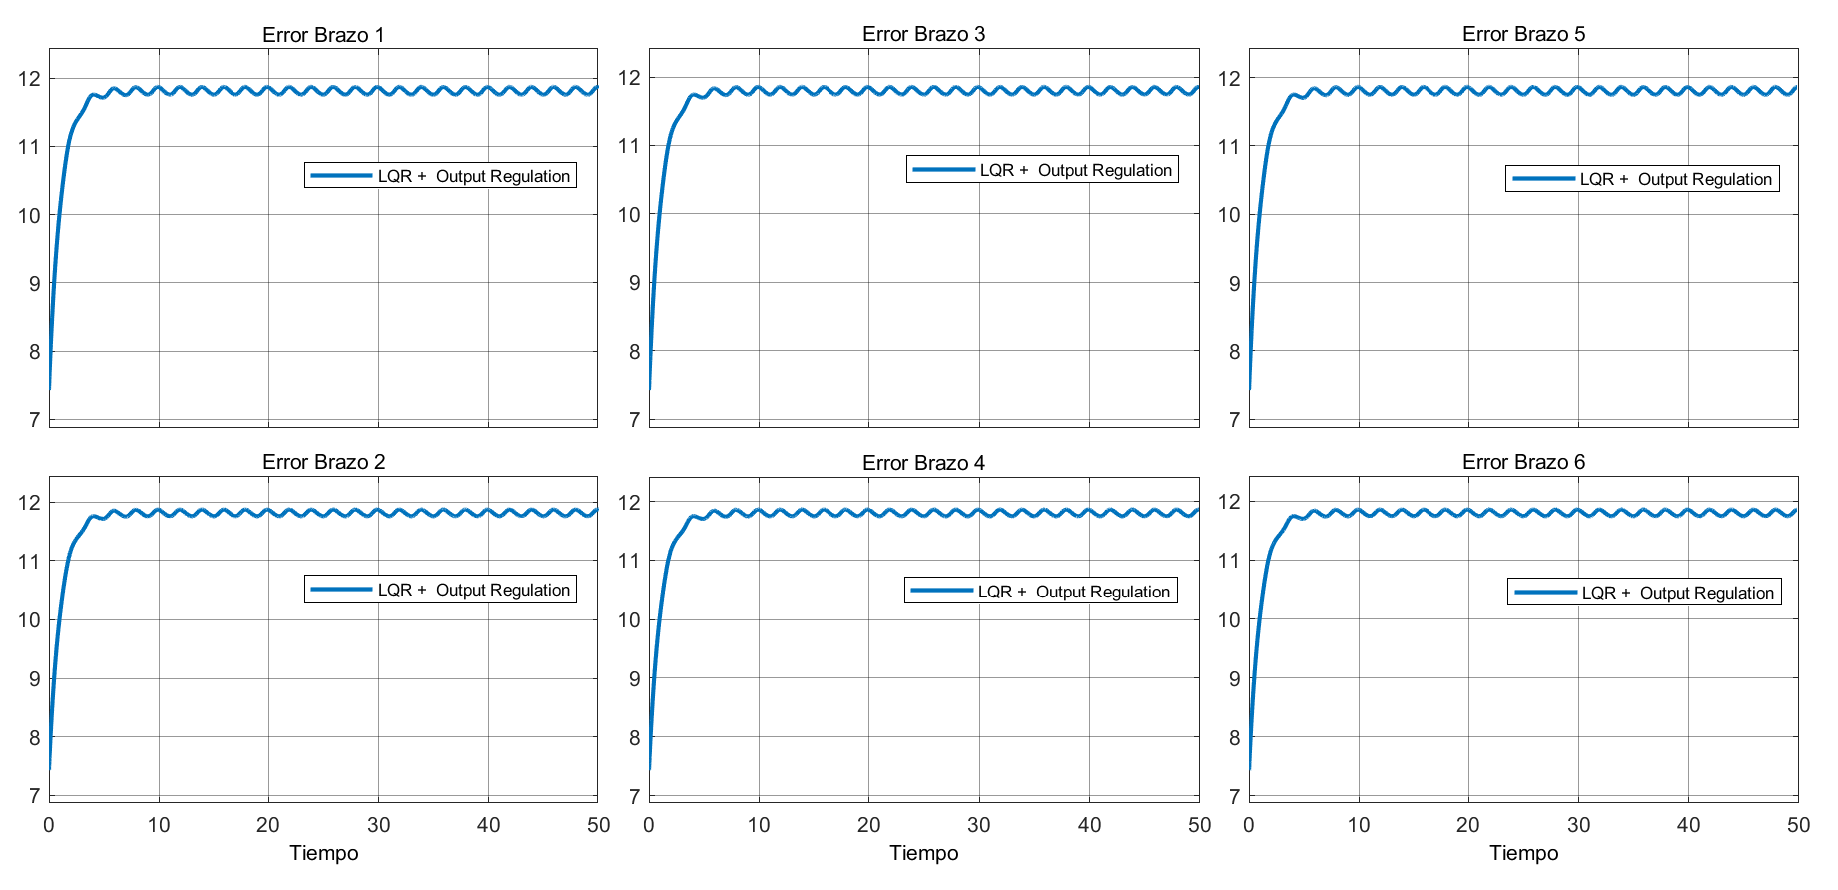
\includegraphics[width=0.9\columnwidth]{Results/lqrOR_frec_fija/lqr_sys_real_frec_fija.eps}
    \caption{Error de seguimiento (cm) LQR + Output Regulation sistema no-lineal, referencia frecuencia fija.}
    \label{fig:lqrOR_real_frec_fija}
\end{figure}

%--------------------------------------------------
\subsection{Referencia sinusoidal Nro.2 frecuencia, amplitud y fase variable}

Se define la referencia Nro.2 a seguir de cada brazo, con escalones y sinusoidales de distinta amplitud, frecuencia, y fase:
\begin{equation}
    l_{ref2}(t) = \begin{bmatrix}
        4 sin(0.5\pi t) + 8\\
        sin(\pi t) + 10\\
        sin(0.5\pi t) + 10\\
        sin(\pi t) + 10\\
        sin(0.5\pi t) + 10\\
        sin(\pi t) + 10\\
    \end{bmatrix}
\end{equation}

Se establecen así los parámetros de la referencia de amplitud, frecuencia y fase variable:
\begin{itemize}
    \item amplitud escalón $\Upsilon_{step1}=8$ y $\Upsilon_{step2}=\Upsilon_{step3}=\Upsilon_{step4}=\Upsilon_{step5}=\Upsilon_{step6}=10$.
    \item amplitud sinusoidal $\Upsilon_{sin1}=4$ y $\Upsilon_{sin2}=\Upsilon_{sin3}=\Upsilon_{sin4}=\Upsilon_{sin5}=\Upsilon_{sin6}=1$,\\ 
    frecuencia $\theta_1=\theta_3=\theta_5=0.5\pi$ y $\theta_2=\theta_4=\theta_6=\pi$, \\
    fase $\phi_1=\phi_2=\phi_3=\phi_4=\phi_5=\phi_6=0$.
\end{itemize}
 

Con los parámetros obtenidos de la referencia se modela su sistema exógeno de \ref{eq:sys_ref_variable}. Con el sistema exógeno de la referencia y los parámetros del sistema \ref{eq:sysStewart_outputregulation} de la plataforma Stewart, se obtiene la matriz feedforward $K_v$ del control para la referencia sinusoidal Nro.2:

\begin{multline}
    K_v = \scalebox{0.75}{$\left[ \begin{matrix}
        59.103 &	28.233 &	15.377 &	\textrm{-}29.820 &	\textrm{-}2.125 &	\textrm{-}0.547 &	\textrm{-}10.957 &	\textrm{-}1.023 &	\textrm{-}0.281 &	20.854 &	1.634 &	0.394 \\
        \textrm{-}23.809 &	\textrm{-}11.047 &	\textrm{-}2.181 &	73.682 &	6.050 &	3.842 &	\textrm{-}17.338 &	\textrm{-}1.749 &	\textrm{-}0.088 &	\textrm{-}4.819 &	\textrm{-}0.192 & \textrm{-}0.118 \\
        \textrm{-}3.875 &	\textrm{-}1.648 &	\textrm{-}0.475 &	\textrm{-}17.338 &	\textrm{-}1.793 &	\textrm{-}0.088 &	73.946 &	7.065 &	3.845 &	\textrm{-}29.876 &	\textrm{-}2.130 &	\textrm{-}0.547 \\
        16.725 &	7.911 &	1.582 &	\textrm{-}11.006 &	\textrm{-}0.811 &	\textrm{-}0.282 &	\textrm{-}29.907 &	\textrm{-}2.776 &	\textrm{-}0.548 &	74.108 &	6.092 &	3.846 \\
        \textrm{-}8.941 &	\textrm{-}4.181 &	\textrm{-}1.134 &	20.881 &	1.636 &	0.396 &	\textrm{-}4.822 &	\textrm{-}0.410 &	\textrm{-}0.118 &	\textrm{-}17.541 &	\textrm{-}1.813 &	\textrm{-}0.089 \\
        \textrm{-}13.878 &	\textrm{-}6.998 &	\textrm{-}0.353 &	\textrm{-}4.740 &	\textrm{-}0.184 &	\textrm{-}0.118 &	20.868 &	1.974 &	0.395 &	\textrm{-}11.063 &	\textrm{-}0.816 &	\textrm{-}0.282 \\
    \end{matrix} \right.$} \\
    \scalebox{0.75}{$\left. \begin{matrix}
        \textrm{-}4.997 &	\textrm{-}0.427 &	\textrm{-}0.120 &	\textrm{-}17.298 &	\textrm{-}1.789 &	\textrm{-}0.087 \\
        20.750 &	1.962 &	0.393 &	\textrm{-}10.849 &	\textrm{-}0.795 &	\textrm{-}0.280 \\
        \textrm{-}10.985 &	\textrm{-}1.026 &	\textrm{-}0.281 &	20.859 &	1.634 &	0.395 \\
        \textrm{-}17.514 &	\textrm{-}1.766 &	\textrm{-}0.089 &	\textrm{-}4.902 &	\textrm{-}0.200 &	\textrm{-}0.119 \\
        74.255 &	7.096 &	3.847 &	\textrm{-}29.912 &	\textrm{-}2.134 &	\textrm{-}0.548 \\
        \textrm{-}29.848 &	\textrm{-}2.770 &	\textrm{-}0.547 &	73.887 &	6.070 &	3.845 \\
    \end{matrix} \right]$}
\end{multline}


\subsubsection{Simulación Sistema Lineal}

En la Figura \ref{fig:lqrOR_lineal_frec_variable} se puede apreciar el error de seguimiento de los brazos actuadores del sistema lineal. Como se puede notar, el efecto del Output Regulation funciona perfectamente al seguir a la referencia sinusoidal de amplitud, frecuencia y fase variable, mostrando un error cero en estado estacionario para el sistema linealizado.
\begin{figure}[H]
\centering
    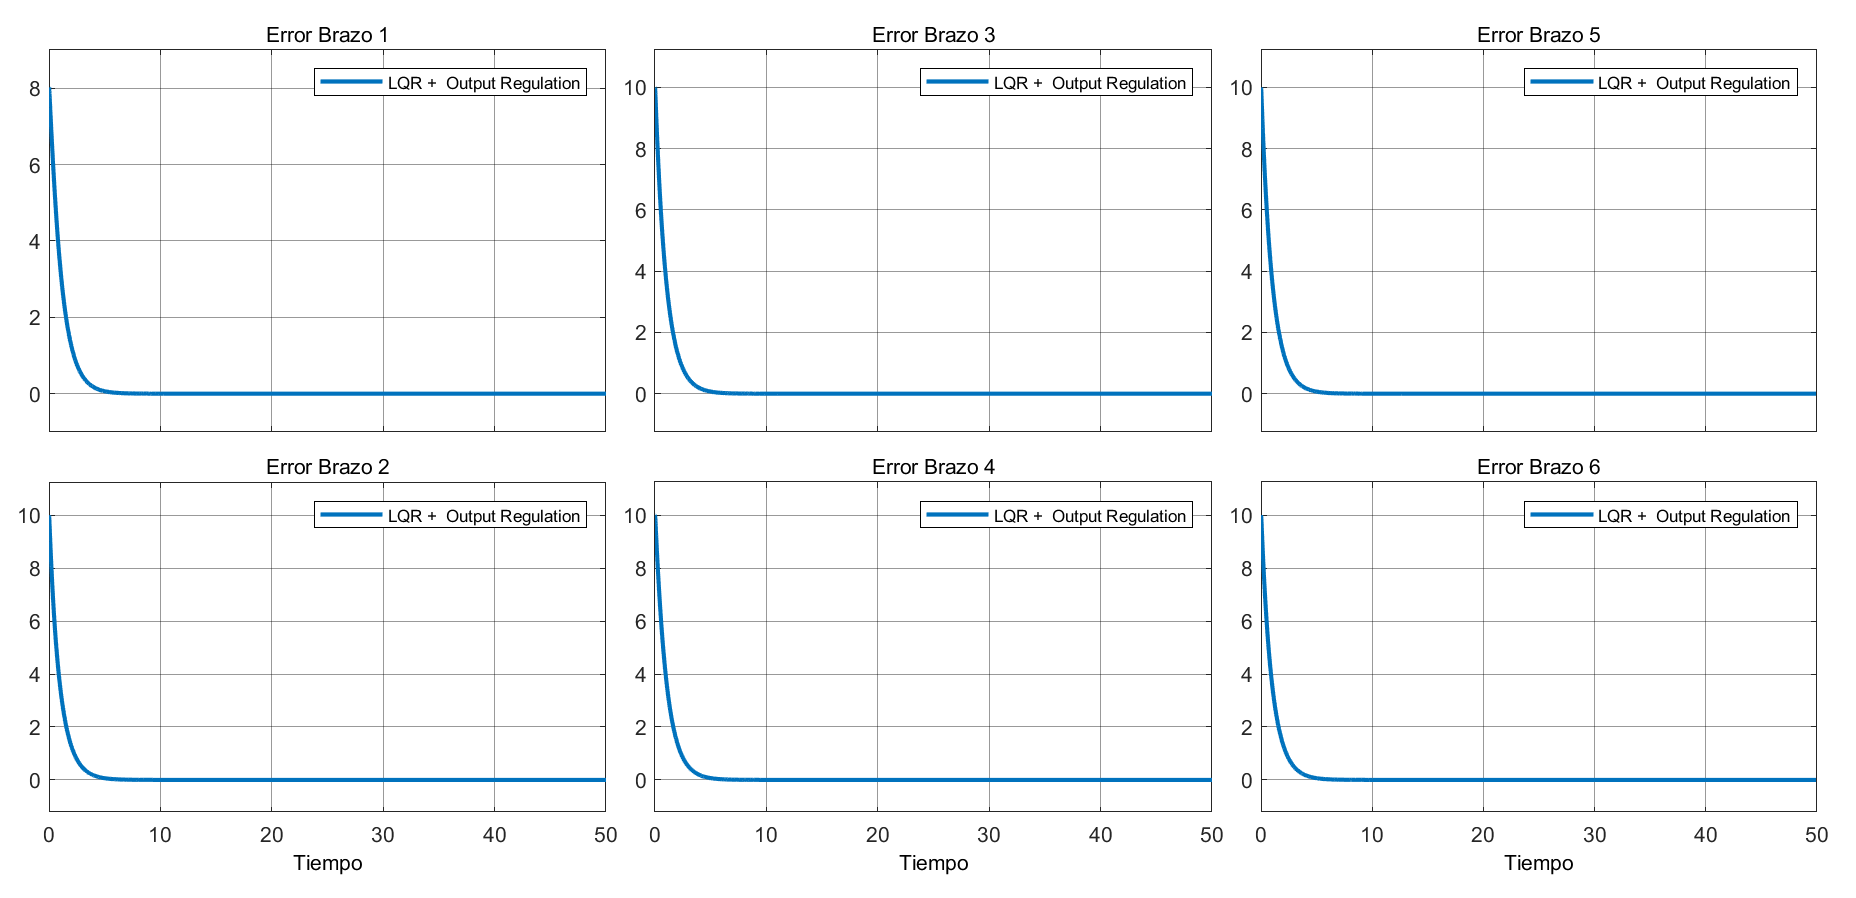
\includegraphics[width=0.87\columnwidth]{Results/lqrOR_frec_variable/lqr_sys_lineal_frec_variable.eps}
    \caption{Error de seguimiento (cm) LQR + Output Regulation sistema lineal, referencia frecuencia variable.}
    \label{fig:lqrOR_lineal_frec_variable}
\end{figure}

\subsubsection{Simulación Sistema No-Lineal}

Se utiliza el sistema no-lineal de la plataforma Stewart para la simulación, ilustrando los errores de seguimiento de los brazos en la Figura \ref{fig:lqrOR_real_frec_variable}.

Como se puede notar, se obtiene un error considerable en todos los brazos actuadores. Cada gráfica posee un valor de error constante junto a oscilaciones que se diferencian entre si. 
Por mucho que la nueva referencia sinusoidal de frecuencia variable haya sido incluida en el problema de Output Regulation, no fue suficiente para garantizar un seguimiento adecuado de esta referencia, es decir, error estacionario cero.

\begin{figure}[H]
\centering
    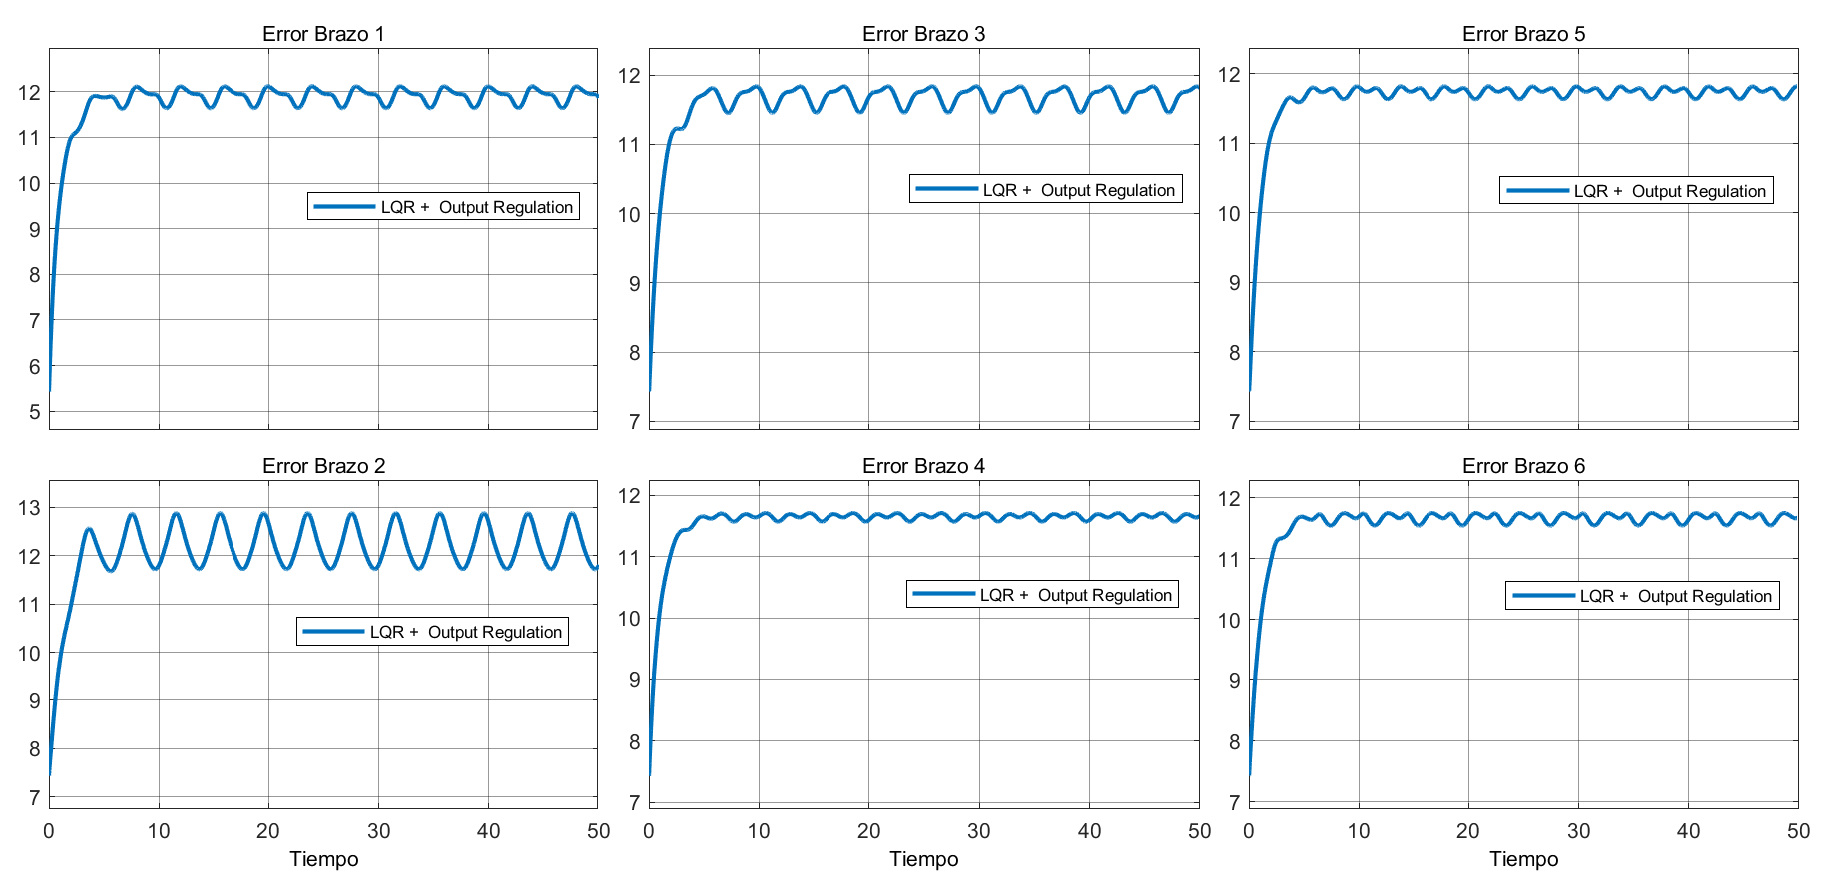
\includegraphics[width=0.87\columnwidth]{Results/lqrOR_frec_variable/lqr_sys_real_frec_variable.eps}
    \caption{Error de seguimiento (cm) LQR + Output Regulation sistema no-lineal, referencia frecuencia variable.}
    \label{fig:lqrOR_real_frec_variable}
\end{figure}


Con los resultados obtenidos en ambos casos de las referencias sinusoidal Nro.1 y Nro.2 (frecuencia fija y variable), podemos concluir que no es suficiente un controlador LQR con Output Regulation para el seguimiento sinusoidal. Las simulaciones con las plantas lineales dieron buenos resultados, pero al momento de modelar con el sistema no-lineal los resultados no eran los esperados. En primer lugar, se obtuvo un valor constante presente en todas las gráficas de error. En segundo lugar, un factor oscilante se presento también en todos estos errores. Tanto el valor constante como el oscilante, deben tratar de ser erradicados para lograr un control eficiente. 

Para lograr corregir los 2 defectos anteriores, se propone a continuación 2 ajustes al diseño de control desarrollado para el seguimiento a referencia sinusoidal. 




%###############################################
%###############################################
%###############################################
 \section{Diseño control LQI con Output Regulation posición velocidad}
\lhead[\thepage]{Sección \thesection. LQI con Output Regulation}

Se proponen 2 ajustes al control anterior para mejorar el desempeño y corregir los errores obtenidos:
\begin{itemize}
    \item \textbf{\underline{Control LQI:}} Adición de la integral del error como estado extra al sistema, para garantizar error de posición cero en estado estacionario para la componente constante de la referencia. Con esto se eliminará cualquier tipo de constante otorgada por parte de la referencia o de perturbaciones en el caso de que el sistema posea.

    \item \textbf{\underline{Output Regulation con posición y velocidad:}} Como la medición de la velocidad de los brazos actuadores esta disponible, se puede utilizar junto a la posición y velocidad de la referencia ya conocida, para aumentar la precisión en la regulación empleada para el seguimiento sinusoidal. De esta forma, se podrá disminuir aun más el error de seguimiento de la componente sinusoidal.
\end{itemize}

Se agrega la integral del error como estado extra, teniendo un estado aumentado al igual como se desarrolló en la sección \ref{sec:lqi_stewart} del capítulo \ref{cap:mimoPID}. Con el sistema aumentado LQI \ref{eq:sys_aumentado_lqi} y el sistema lineal \ref{eq:sysStewart_outputregulation} de la plataforma Stewart se tiene:

\begin{equation} 
    \begin{bmatrix}
        \dot{\xi}(t) \\ \dot{\xi}_{int}(t)
    \end{bmatrix} = \underbrace{\begin{bmatrix}
        A_0 & 0 \\ -C_0 & 0 
    \end{bmatrix}}_{A_a} \begin{bmatrix}
        \xi(t) \\ \xi_{int}(t)
    \end{bmatrix} + \underbrace{\begin{bmatrix}
        B_0 \\ 0
    \end{bmatrix}}_{B_a} u(t)
\end{equation}
donde $\xi_{int}(t) = \int e(t) dt= \int (r(t)-y(t)) dt = \int (r(t)-C_0 \xi(t)) dt$ es la integral del error de seguimiento de posición, y el nuevo estado aumentado definido como $z(t) = \begin{bmatrix} \xi(t)^\top & \xi_{int}(t)^\top\end{bmatrix}^\top$.

Resolviendo para la ley de control LQI como se desarrolla en la sección \ref{sec:lqicontrol} del capítulo \ref{cap:Notación y preliminares}, se obtienen las matrices de realimentación $K_\xi$ y $K_{int}$:
\begin{equation}
    u(t) = -K_\xi \xi(t) - K_{int} \xi_{int}(t)
\end{equation}

Posteriormente, se define la referencia incluyendo la velocidad como la derivada de la posición:
\begin{equation}
    \begin{bmatrix}
        l_{ref}(t) \\ \dot{l}_{ref}(t)
    \end{bmatrix} = \begin{bmatrix}
        \Upsilon_{pos1} sin(\theta_1 t + \phi_1) + \Upsilon_{step1}\\
        \Upsilon_{pos2} sin(\theta_2 t + \phi_2) + \Upsilon_{step2}\\
        \Upsilon_{pos3} sin(\theta_3 t + \phi_3) + \Upsilon_{step3}\\
        \Upsilon_{pos4} sin(\theta_4 t + \phi_4) + \Upsilon_{step4}\\
        \Upsilon_{pos5} sin(\theta_5 t + \phi_5) + \Upsilon_{step5}\\
        \Upsilon_{pos6} sin(\theta_6 t + \phi_6) + \Upsilon_{step6}\\
        \Upsilon_{pos1} \theta_1 cos(\theta_1 t + \phi_1)\\
        \Upsilon_{pos2} \theta_2 cos(\theta_2 t + \phi_2)\\
        \Upsilon_{pos3} \theta_3 cos(\theta_3 t + \phi_3)\\
        \Upsilon_{pos4} \theta_4 cos(\theta_4 t + \phi_4)\\
        \Upsilon_{pos5} \theta_5 cos(\theta_5 t + \phi_5)\\
        \Upsilon_{pos6} \theta_6 cos(\theta_6 t + \phi_6)\\
    \end{bmatrix}
\end{equation}

Se modela la referencia como sistema exógeno de la forma:
\begin{align} \label{eq:ref_exogeno_LQI_OR}
    \dot{v}(t) & = H_v v(t), \notag \\
    \begin{bmatrix}
        l_{ref}(t) \\ \dot{l}_{ref}(t)
    \end{bmatrix} & = C_v v(t)
\end{align}
donde 
\begin{gather}
    H_v = \begin{bmatrix}
        H_{v1} & \hdots & 0 \\
        \vdots & \ddots & \vdots \\ 
        0 & \hdots & H_{v6}
    \end{bmatrix}, 
    \quad \textrm{con } \quad
    H_{vi} = \begin{bmatrix}
        0 & 0 & 0 \\
        0 & 0 & 1 \\
        0 & -\theta_i^2 & 0
    \end{bmatrix},  \\
    C_v = \begin{bmatrix}
        C_{v1\_pos} & \hdots & 0 \\
        \vdots & \ddots & \vdots \\ 
        0 & \hdots & C_{v6\_pos} \\
        C_{v1\_vel} & \hdots & 0 \\
        \vdots & \ddots & \vdots \\ 
        0 & \hdots & C_{v6\_vel}
    \end{bmatrix}, \notag \\
    \quad \textrm{con } \quad
    C_{vi\_pos} = \begin{bmatrix}
        \Upsilon_{step\textrm{ }i} & \Upsilon_{pos\textrm{ }i} & 0
    \end{bmatrix},
    \quad 
    C_{vi\_vel} = \begin{bmatrix}
        0 & 0 & \theta_i \Upsilon_{pos\textrm{ }i}
    \end{bmatrix}, \\
    v(0) = \begin{bmatrix}
        \begin{bmatrix} 1 & sin(\phi_1) & cos(\phi_1) \end{bmatrix} & \hdots & \begin{bmatrix} 1 & sin(\phi_6) & cos(\phi_6) \end{bmatrix} 
    \end{bmatrix}, \quad
    \textrm{tal que } i = 1,\hdots,6 \notag
\end{gather}

Con la nueva referencia con velocidad incluida y la nueva matriz de los estados internos del sistema $(-K_\xi)$ (se incluye signo negativo), se resuelven las ecuaciones de regulación para $X$ y $U$ (demostrado en Apéndice \ref{appen1}) en el problema de Output Regulation de posición y velocidad:

\begin{align}
    X H_v = A_0 X + B_0 U \notag \\
    0 = C_0 X + D_0 U - C_v 
\end{align}

Con $A_0, B_0, C_0, D_0$ las matrices del sistema lineal \ref{eq:sysStewart_outputregulation} de la plataforma Stewart, donde $C_0$ nos permite medir directamente posición y velocidad de los brazos. Además $C_v$ corresponde a la referencia deseada de la posición y de la velocidad de los brazos.

Con $X$ y $U$ obtenidos se despeja $K_v$ desde la igualdad $K_v = U - (-K_\xi) X$.

Finalmente, se obtiene la ley de control LQI con Output Regulation posición velocidad para referencias sinusoidales de la forma:

\begin{equation}
    u(t) = -K_\xi \xi(t) - K_{int} \xi_{int}(t) + K_v v(t)
\end{equation}
con $\xi(t)$ los estados de la plataforma Stewart (posición y velocidad de brazos), $\xi_{int}(t)$ el estado de la integral del error de posición y $v(t)$ el estado interno del sistema exógeno de la referencia.

En la Figura \ref{fig:lqi_OR_stewart_scheme} se puede ilustrar el nuevo esquema de control LQI con Output Regulation posición velocidad. 

\begin{figure}[ht]
\centering
    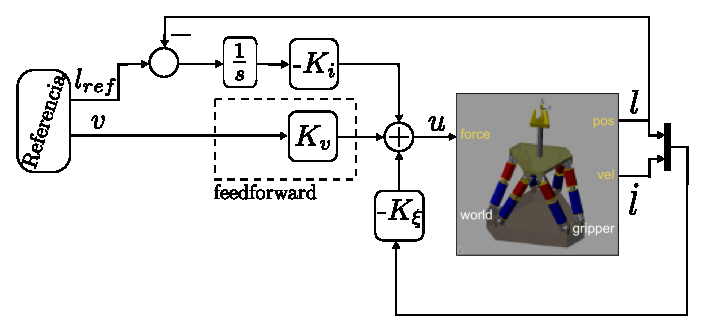
\includegraphics[width=0.8\columnwidth]{Figures/Output_Regulation/lqi_OR_stewart_scheme.eps}
    \caption{Esquema de control LQI con Output Regulation posición velocidad para la plataforma Stewart.}
    \label{fig:lqi_OR_stewart_scheme}
\end{figure}

 \section{Resultados de simulación control LQI con Output Regulation posición velocidad}
\lhead[\thepage]{Sección \thesection. Resultados de simulación control LQI con Output Regulation}

Los resultados de simulación del control LQI con Output Regulation posición velocidad para seguimiento sinusoidal, se compararán con el controlador de mejor desempeño del capítulo \ref{cap:mimoPID} anterior. Recordando, el controlador MIMO PID Full del capítulo \ref{cap:mimoPID} demostraba tener un mejor seguimiento de la referencia, así como mejores índices de desempeño en comparación con sus versiones descentralizadas. El principal problema que presenta es en el seguimiento de referencia sinusoidal, ya que la magnitud del error de seguimiento es significativo.

\begin{remark}
Las matrices $K_P$, $K_D$ y $K_I$ del controlador MIMO PID Full utilizadas son las mismas mostradas en \ref{eq:KP_mimoPID}, \ref{eq:KD_mimoPID} y \ref{eq:KI_mimoPID}, en los resultados del Caso 2 de la sección \ref{sec:resultados_mimoPID} del capítulo \ref{cap:mimoPID}.
\end{remark}

Se utilizan las matrices $A_0, B_0, C_0, D_0$ del sistema lineal \ref{eq:sysStewart_outputregulation} de la plataforma Stewart.

Para el diseño del control LQI con Output Regulation, se utilizan las siguientes matrices $Q$ y $R$ para la obtención de las matrices de realimentación:
\begin{equation}
    Q = \begin{bmatrix} C_0^\top C_0 & 0 \\ 0 & 100\cdot I_{6\times6} \end{bmatrix}, \qquad R = 0.1\cdot I_{6\times6} 
\end{equation}
La explicación del $Q$ anterior es la misma mencionada en el capítulo \ref{cap:mimoPID}, es decir, se ponderan los estados correspondientes a la integral del error por sobre los demás para así darle más importancia al seguimiento de la referencia. Por otro lado, la matriz $R$ utilizada es de baja ponderación para la señal de actuación, para así no restringir demasiado su efecto en el sistema.

Con $Q$ y $R$ dados, las matrices de realimentación $K_\xi$ y $K_{int}$ para el control LQI con Output Regulation posición velocidad son:

\begin{equation}
    K_\xi = \scalebox{0.8}{$\begin{bmatrix}
        24.037 &	\textrm{-}6.357 &	\textrm{-}2.141 &	3.812 &	\textrm{-}1.493 &	\textrm{-}2.746 & 4.150 &	\textrm{-}0.710 &	\textrm{-}0.304 &	0.443 &	\textrm{-}0.194 &	\textrm{-}0.038 \\
        \textrm{-}6.363 &	24.013 &	\textrm{-}2.739 &	\textrm{-}1.479 &	3.807 &	\textrm{-}2.125 & \textrm{-}0.709 &	4.148 &	\textrm{-}0.038 &	\textrm{-}0.193 &	0.442 &	\textrm{-}0.303 \\
        \textrm{-}1.478 &	\textrm{-}2.785 &	24.078 &	\textrm{-}6.361 &	\textrm{-}2.137 &	3.807 & \textrm{-}0.193 &	\textrm{-}0.038 &	4.158 &	\textrm{-}0.710 &	\textrm{-}0.304 &	0.443 \\
        3.784 &	\textrm{-}2.159 &	\textrm{-}6.351 &	24.089 &	\textrm{-}2.786 &	\textrm{-}1.467 & 0.444 &	\textrm{-}0.305 &	\textrm{-}0.711 &	4.151 &	\textrm{-}0.039 &	\textrm{-}0.193 \\
        \textrm{-}2.181 &	3.768 &	\textrm{-}1.452 &	\textrm{-}2.777 &	24.093 &	\textrm{-}6.341 & \textrm{-}0.306 &	0.445 &	\textrm{-}0.192 &	\textrm{-}0.040 &	4.152 &	\textrm{-}0.711 \\
        \textrm{-}2.773 &	\textrm{-}1.461 &	3.799 &	\textrm{-}2.136 &	\textrm{-}6.370 &	24.065 & \textrm{-}0.039 &	\textrm{-}0.192 &	0.443 &	\textrm{-}0.304 &	\textrm{-}0.710 &	4.150 \\
    \end{bmatrix}$}
\end{equation}

\begin{equation}
    K_{int} = \begin{bmatrix}
    	\textrm{-}31.611 &	0.005 &	0.577 &	0.004 &	\textrm{-}0.594 &	\textrm{-}0.005 \\
    	\textrm{-}0.005 &	\textrm{-}31.611 &	\textrm{-}0.0002 &	\textrm{-}0.594 & 0.012 & 0.576 \\
    	\textrm{-}0.588 &	0.0006 &	\textrm{-}31.611 &	\textrm{-}0.002 &	0.582 &	0.0005 \\
    	\textrm{-}0.004 &	0.584 &	0.002 &	\textrm{-}31.611 &	\textrm{-}0.002 &	\textrm{-}0.592 \\
    	0.583 &	\textrm{-}0.012 &	\textrm{-}0.593 &	0.002 &	\textrm{-}31.611 &	0.005 \\
    	0.005 &	\textrm{-}0.587 &	\textrm{-}0.0008 &	0.581 &	\textrm{-}0.005 &	\textrm{-}31.611 \\
    \end{bmatrix}
\end{equation}

%--------------------------------------------------
\subsection{Referencia sinusoidal Nro.1 frecuencia fija}

Se establece la referencia sinusoidal Nro.1 de frecuencia fija, para el seguimiento de los brazos actuadores:

\begin{equation}
    \begin{bmatrix}
        l_{ref1}(t) \\ \dot{l}_{ref1}(t)
    \end{bmatrix} = \begin{bmatrix}
        2 sin(\pi t ) + 10\\
        2 sin(\pi t ) + 10\\
        2 sin(\pi t ) + 10\\
        2 sin(\pi t ) + 10\\
        2 sin(\pi t ) + 10\\
        2 sin(\pi t ) + 10\\
        2 \pi cos(\pi t )\\
        2 \pi cos(\pi t )\\
        2 \pi cos(\pi t )\\
        2 \pi cos(\pi t )\\
        2 \pi cos(\pi t )\\
        2 \pi cos(\pi t )\\
    \end{bmatrix}
\end{equation}

Se definen así los siguientes parámetros de la referencia:
\begin{itemize}
    \item amplitud escalón $\Upsilon_{step1}=\Upsilon_{step2}=\Upsilon_{step3}=\Upsilon_{step4}=\Upsilon_{step5}=\Upsilon_{step6}=10$.
    \item amplitud sinusoidal posición $\Upsilon_{pos1}=\Upsilon_{pos2}=\Upsilon_{pos3}=\Upsilon_{pos4}=\Upsilon_{pos5}=\Upsilon_{pos6}=2$, \\
    frecuencia $\theta_1=\theta_2=\theta_3=\theta_4=\theta_5=\theta_6=\pi$, \\
    fase $\phi_1=\phi_2=\phi_3=\phi_4=\phi_5=\phi_6=0$.
\end{itemize}

Con los parámetros obtenidos de la referencia se modela su sistema exógeno de \ref{eq:ref_exogeno_LQI_OR}. Con el sistema exógeno de la referencia y los parámetros del sistema \ref{eq:sysStewart_outputregulation} de la plataforma Stewart, se obtiene la matriz feedforward $K_v$ del control para la referencia sinusoidal Nro.1:

\begin{multline}
    K_v = \scalebox{0.75}{$\left[\begin{matrix}
        179.928 &  33.348 &  8.300 & \textrm{-}24.813 & \textrm{-}3.247 & \textrm{-}1.421 & \textrm{-}11.375 & \textrm{-}1.695  & \textrm{-}0.608 &  16.930 & 2.482 & 0.887 \\
      \textrm{-}24.745 &  \textrm{-}3.233 &  \textrm{-}1.419 & 179.818 &  33.326  &  8.297 &  \textrm{-}7.309  & \textrm{-}1.579  & \textrm{-}0.077 &  \textrm{-}4.416  & \textrm{-}0.303  & \textrm{-}0.386 \\
       \textrm{-}4.446 &  \textrm{-}0.309  & \textrm{-}0.387 &  \textrm{-}7.312 &  \textrm{-}1.580 &  \textrm{-}0.077 & 179.974 &  33.357  &  8.301 & \textrm{-}24.837 &  \textrm{-}3.252 &  \textrm{-}1.421 \\
       16.989  &  2.494 &   0.889 & \textrm{-}11.429 &  \textrm{-}1.706 &  \textrm{-}0.610 & \textrm{-}24.863 &  \textrm{-}3.257 &  \textrm{-}1.422 & 180.067 &  33.376  &  8.303 \\
      \textrm{-}11.511 &  \textrm{-}1.722 &  \textrm{-}0.612 &  16.997  &  2.495  &  0.890 &  \textrm{-}4.395 &  \textrm{-}0.299  & \textrm{-}0.385 &  \textrm{-}7.448  & \textrm{-}1.607 &  \textrm{-}0.080 \\
       \textrm{-}7.342 &  \textrm{-}1.586 &  \textrm{-}0.078 &  \textrm{-}4.388 &  \textrm{-}0.297 &  \textrm{-}0.385 &  16.937  &  2.483  &  0.887 & \textrm{-}11.422 &  \textrm{-}1.704 &  \textrm{-}0.609 
    \end{matrix}\right.$} \\
    \scalebox{0.75}{$\left. \begin{matrix}
        \textrm{-}4.508 &  \textrm{-}0.321 & \textrm{-}0.388 & \textrm{-}7.281 & \textrm{-}1.574 & \textrm{-}0.076 \\
        16.846  &  2.465 &   0.885 & \textrm{-}11.311 &  \textrm{-}1.682 & \textrm{-}0.606 \\
        \textrm{-}11.382 &  \textrm{-}1.696 &  \textrm{-}0.608 &  16.928 &   2.481 & 0.887 \\
        \textrm{-}7.418  & \textrm{-}1.601 &  \textrm{-}0.079 &  \textrm{-}4.438 &  \textrm{-}0.307 & \textrm{-}0.386 \\
        180.128 &  33.388 &   8.304 & \textrm{-}24.866 &  \textrm{-}3.258 & \textrm{-}1.422 \\
        \textrm{-}24.799  & \textrm{-}3.244 &  \textrm{-}1.420 & 179.937 &  33.350 & 8.300
    \end{matrix}\right]$}
\end{multline}

Para un tiempo de simulación de $T_{sim}=50(s)$ se obtienen las gráficas de error de posición y fuerza de actuación mostradas en las Figuras \ref{fig:lqiOR_error_frec_fija} y \ref{fig:lqiOR_fuerza_frec_fija} respectivamente. 
En primera instancia si comparamos el error del control LQI Output Regulation (Figura \ref{fig:lqiOR_error_frec_fija}) con el error del control LQR Output Regulation (Figura \ref{fig:lqrOR_real_frec_fija}), notamos una mejora considerable al utilizar el integrador del control LQI, ya que elimina el valor constante que presenta el error del control LQR. Por otro lado, es evidente que el control MIMO PID Full no es capaz de seguir correctamente a la referencia sinusoidal evidenciado en los altos valores del error de seguimiento que posee. Finalmente, al utilizar Output Regulation podemos notar que el error en cada brazo disminuye considerablemente con la matriz feedforward $K_v$ de la referencia. Esta matriz permite el seguimiento de la señal de manera más eficiente como se aprecia en la gráfica, logrando magnitudes del error muy pequeñas del orden de los $0.02$. 

Con respecto a las fuerzas aplicadas en los brazos actuadores (Figura \ref{fig:lqiOR_fuerza_frec_fija}), podemos notar que el controlador MIMO PID Full posee actuaciones más pequeñas que el control LQI con Output Regulation. Por mucho que la actuación sea levemente menor, el control MIMO PID Full no es suficiente para el seguimiento sinusoidal como se aprecia en la gráfica del error. La diferencia de actuación con el control LQI Output Regulation radica en que este está enfocado en seguir a la referencia sinusoidal de mejor manera, por ende, necesita de más actuación para el control.
\newpage
\begin{figure}[H]
\centering
    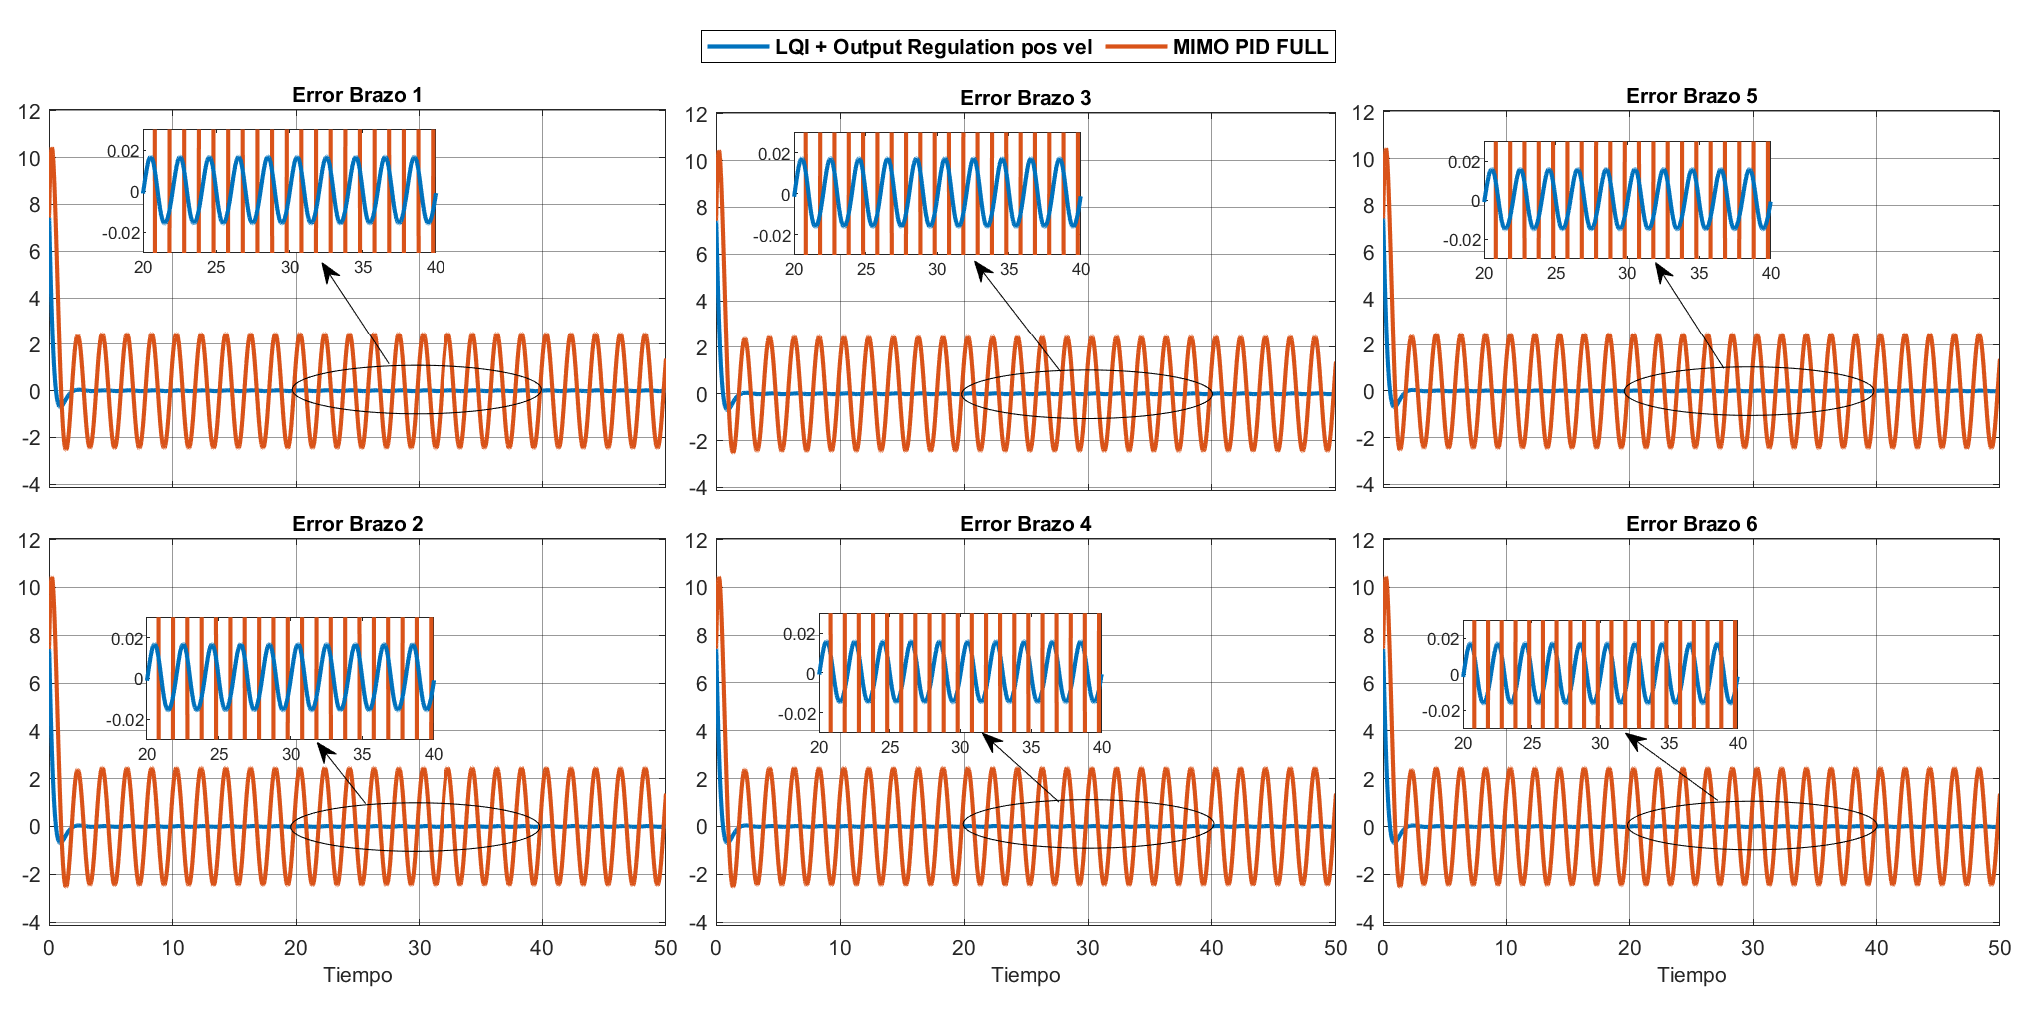
\includegraphics[width=1\columnwidth]{Results/LQI_OR_frec_fija/error_frec_fija.eps}
    \caption{Error de seguimiento (cm) LQI+OR v/s MIMO PID Full, referencia frecuencia fija.}
    \label{fig:lqiOR_error_frec_fija}
\end{figure}

\begin{figure}[H]
\centering
    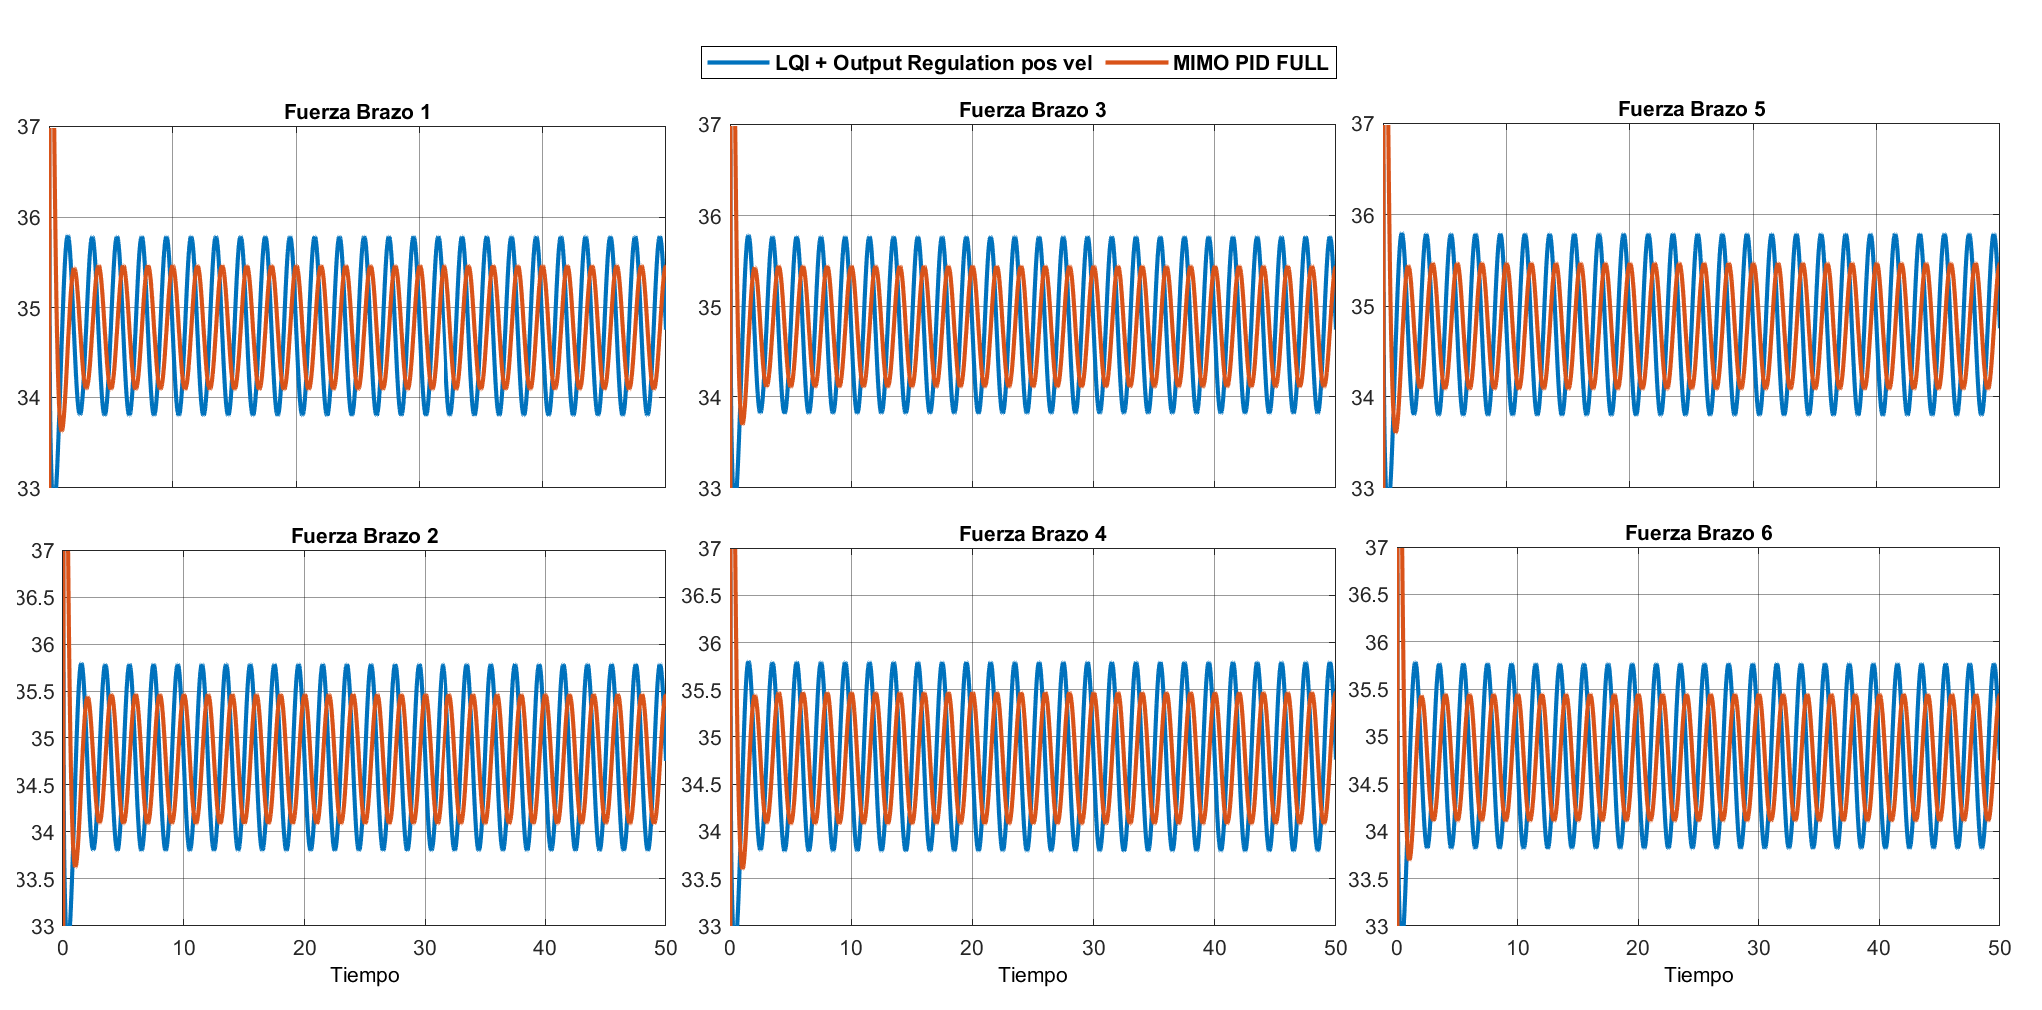
\includegraphics[width=1\columnwidth]{Results/LQI_OR_frec_fija/fuerza_frec_fija.eps}
    \caption{Fuerza de actuación (N) LQI+OR v/s MIMO PID Full, referencia frecuencia fija.}
    \label{fig:lqiOR_fuerza_frec_fija}
\end{figure}

\newpage
%--------------------------------------------------
\subsection{Referencia sinusoidal Nro.2 frecuencia, amplitud y fase variable}

Se establece la referencia sinusoidal Nro.2 de frecuencia, amplitud y fase variable, para el seguimiento de los brazos actuadores:

\begin{equation}
    \begin{bmatrix}
        l_{ref2}(t) \\ \dot{l}_{ref2}(t)
    \end{bmatrix} = \begin{bmatrix}
        4 sin(0.5\pi t ) + 8\\
        sin(\pi t ) + 10\\
        sin(0.5\pi t ) + 10\\
        sin(\pi t ) + 10\\
        sin(0.5\pi t ) + 10\\
        sin(\pi t ) + 10\\
        4(0.5\pi) cos(0.5\pi t )\\
        \pi cos(\pi t )\\
        0.5\pi cos(0.5\pi t )\\
        \pi cos(\pi t )\\
        0.5\pi cos(0.5\pi t )\\
        \pi cos(\pi t )\\
    \end{bmatrix}
\end{equation}

Se definen así los siguientes parámetros:
\begin{itemize}
    \item amplitud escalón $\Upsilon_{step1}=8$ y $\Upsilon_{step2}=\Upsilon_{step3}=\Upsilon_{step4}=\Upsilon_{step5}=\Upsilon_{step6}=10$.
    \item amplitud sinusoidal posición $\Upsilon_{pos1}=4$ y $\Upsilon_{pos2}=\Upsilon_{pos3}=\Upsilon_{pos4}=\Upsilon_{pos5}=\Upsilon_{pos6}=1$, \\
    frecuencia $\theta_1=\theta_3=\theta_5=0.5\pi$ y $\theta_2=\theta_4=\theta_6=\pi$, \\
    fase $\phi_1=\phi_2=\phi_3=\phi_4=\phi_5=\phi_6=0$.
\end{itemize}

Con los parámetros obtenidos de la referencia se modela su sistema exógeno de \ref{eq:ref_exogeno_LQI_OR}. Con el sistema exógeno de la referencia y los parámetros del sistema \ref{eq:sysStewart_outputregulation} de la plataforma Stewart, se obtiene la matriz feedforward $K_v$ del control para la referencia sinusoidal Nro.2:

\begin{multline}
    K_v = \scalebox{0.75}{$\left[\begin{matrix}
        143.943	& 70.653 &	16.601 &	\textrm{-}24.813	& \textrm{-}1.624 &	\textrm{-}0.711 &	\textrm{-}11.375	& \textrm{-}1.065 &	\textrm{-}0.304 & 	16.931 &	1.241 &	0.444  \\
        \textrm{-}19.796 &	\textrm{-}9.041 &	\textrm{-}2.838 &	179.818 &	16.663 &	4.149 &	\textrm{-}7.309 &	\textrm{-}0.746 &	\textrm{-}0.039 &	\textrm{-}4.417 &	\textrm{-}0.152 &	\textrm{-}0.193  \\
        \textrm{-}3.557 &	\textrm{-}1.489 &	\textrm{-}0.775 &	\textrm{-}7.313 &	\textrm{-}0.790 &	\textrm{-}0.039 &	179.974 &	17.668 &	4.151 &	\textrm{-}24.837 &	\textrm{-}1.626 &	\textrm{-}0.711 \\
        13.591 &	6.344 &	1.779 &	\textrm{-}11.430 &	\textrm{-}0.853 &	\textrm{-}0.305 &	\textrm{-}24.864	& \textrm{-}2.272 &	\textrm{-}0.711 &	180.068 &	16.688 &	4.152 \\
        \textrm{-}9.209 &	\textrm{-}4.315 &	\textrm{-}1.224 &	16.998 &	1.248 &	0.445 &	\textrm{-}4.395 &	\textrm{-}0.367 &	\textrm{-}0.193 &	\textrm{-}7.449 &	\textrm{-}0.804 &	\textrm{-}0.040  \\
        \textrm{-}5.874 &	\textrm{-}2.996 &	\textrm{-}0.157 &	\textrm{-}4.388 &	\textrm{-}0.149 &	\textrm{-}0.193 &	16.937 &	1.581 &	0.444 &	\textrm{-}11.423 &	\textrm{-}0.852 &	\textrm{-}0.305	\\
    \end{matrix}\right.$} \\
    \scalebox{0.75}{$\left.\begin{matrix}
        \textrm{-}4.508 &	\textrm{-}0.378 &	\textrm{-}0.195 &	\textrm{-}7.282 &	\textrm{-}0.787 &	\textrm{-}0.038 \\
        16.847 &	1.572 &	0.443 &	\textrm{-}11.311	& \textrm{-}0.841 &	\textrm{-}0.303 \\
        \textrm{-}11.382 &	\textrm{-}1.066 &	\textrm{-}0.304 &	16.929 &	1.241 &	0.444 \\
        \textrm{-}7.418 &	\textrm{-}0.757 &	\textrm{-}0.040 &	\textrm{-}4.439 &	\textrm{-}0.154 &	\textrm{-}0.193 \\
        180.129 &	17.683 &	4.152 &	\textrm{-}24.867 &	\textrm{-}1.629 &	\textrm{-}0.711 \\
        \textrm{-}24.799 &	\textrm{-}2.266 &	\textrm{-}0.710 &	179.937 &	16.675 &	4.150 \\
    \end{matrix}\right]$}
\end{multline}

Para un tiempo de simulación de $T_{sim}=50(s)$ se obtienen las gráficas de error de posición y fuerza de actuación mostradas en las Figuras \ref{fig:lqiOR_error_frec_variable} y \ref{fig:lqiOR_fuerza_frec_variable} respectivamente. En primera instancia, al comparar el error del control LQI Output Regulation (Figura \ref{fig:lqiOR_error_frec_variable}) con el error del control LQR Output Regulation (Figura \ref{fig:lqrOR_real_frec_variable}) podemos ver que el integrador utilizado en el control LQI logra eliminar completamente la constante presente en todos los errores del control LQR. Por otro lado, en comparación con el control MIMO PID Full se puede notar claramente que el efecto del Output Regulation logra disminuir considerablemente el error de seguimiento en cada brazo, pasando de magnitudes cercanas de $3$ y $1$ para el control MIMO PID Full, a magnitudes cercanas de $0.4$ y $0.1$ respectivamente para el control LQI Output Regulation.

Por otro lado en la Figura \ref{fig:lqiOR_fuerza_frec_variable} , las fuerzas actuadoras del control LQI Output Regulation son levemente mayores que el control MIMO PID Full, ya que posee un objetivo extra que es el seguimiento sinusoidal a diferencia del control MIMO PID Full.

\begin{figure}[H]
\centering
    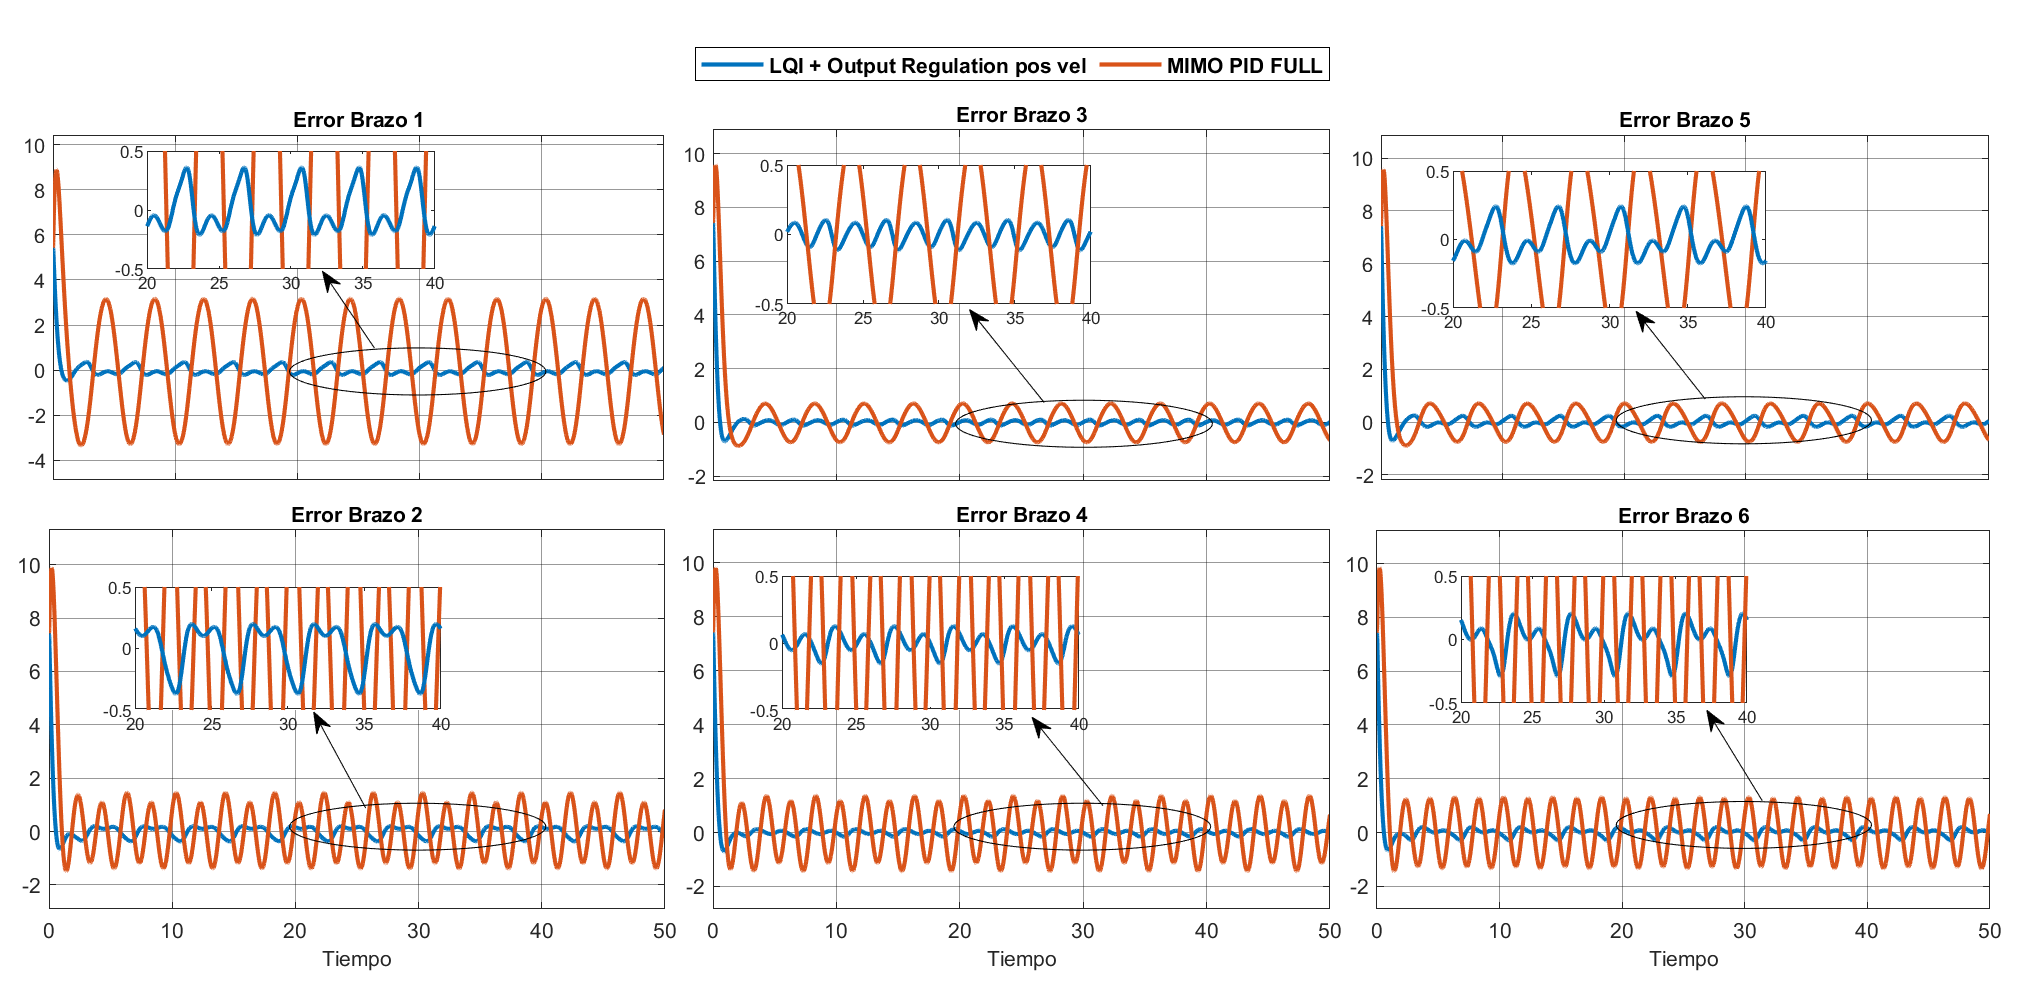
\includegraphics[width=1\columnwidth]{Results/LQI_OR_frec_variable/error_frec_variable.eps}
    \caption{Error de seguimiento (cm) LQI+OR v/s MIMO PID Full, referencia frecuencia variable.}
    \label{fig:lqiOR_error_frec_variable}
\end{figure}
\newpage
\begin{figure}[H]
\centering
    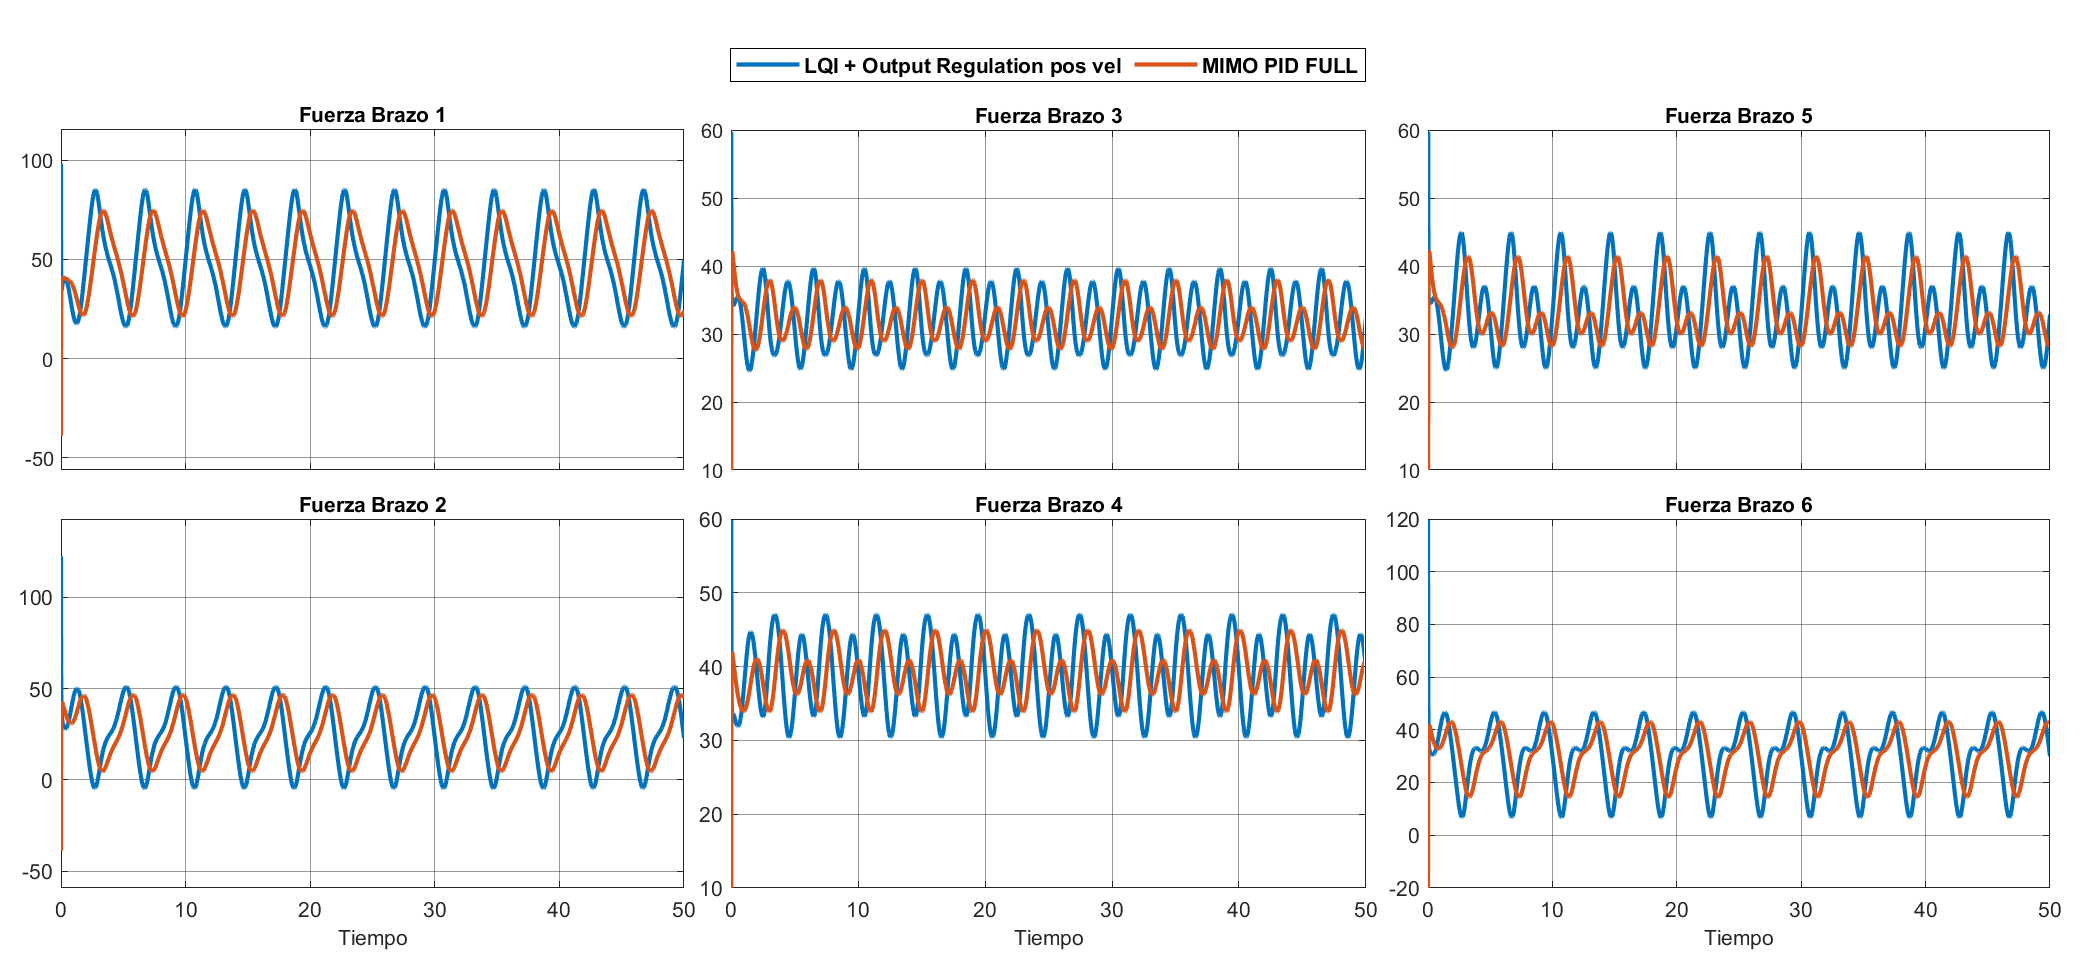
\includegraphics[width=1\columnwidth]{Results/LQI_OR_frec_variable/fuerza_frec_variable.eps}
    \caption{Fuerza de actuación (N) LQI+OR v/s MIMO PID Full, referencia frecuencia variable.}
    \label{fig:lqiOR_fuerza_frec_variable}
\end{figure}

Tanto para las referencias Nro.1 y Nro.2, los errores obtenidos mediante el control LQI con Output Regulation bajaron considerablemente en comparación al controlador MIMO PID Full, evidenciando el efecto del feedforward con la referencia deseada. Se debe notar que, por mucho que se aplica Output Regulation al control, en ninguno de los casos los errores obtenidos son cero. Esto es un punto importante ya que según la definición de Output Regulation garantizaba error cero en estado estacionario. En el caso de la plataforma Stewart, debido a la alta no linealidad que posee, es posible que este sea un factor determinante que impida el error cero en estado estacionario. Otro factor que puede explicar estos resultados, es el no haber pasado las referencias a través del bloque de Cinemática Inversa del capítulo \ref{cap:modeladoStewart}, ya que se tomó como referencia el movimiento de los brazos directamente en lugar de considerar el movimiento de la plataforma superior. Al forzar la trayectoria sin considerar las relaciones dinámicas existentes entre los brazos adyacentes ($1$-$2$ ó $2$-$3$, etc), es posible que se quiera seguir una referencia no realizable, explicando así el error distinto de cero en estado estacionario. Por ejemplo, debido a las condiciones físicas de la plataforma, no es posible tener el brazo 1 en $30(cm)$ de alto mientras el brazo 2 este en $5(cm)$ de alto. Es por esto que, se recomienda asignar el movimiento deseado en la plataforma superior, para posteriormente ser transformado por el bloque de cinemática inversa y así obtener la referencia deseada de los brazos, con el requerimiento necesario de reconocer todos los parámetros de la referencia en su sistema exógeno para poder resolver el problema de Output Regulation en el seguimiento sinusoidal.

Para un análisis más detallado, se consideran nuevamente los índices de desempeño $J_{ISE}$ y $J_u$ de las ecuaciones \ref{eq:indices_desempeño} del capítulo \ref{cap:mimoPID}. El índice $J_{LQI}$ no se considera en esta etapa ya que el controlador MIMO PID al ser sintetizado por control LQI, su costo $J_{LQI}$ es exactamente igual al controlador LQI con Output Regulation, siendo un índice sin información útil para este caso. 

Para un tiempo de simulación $T_{sim}=50(s)$ se muestran los índices de desempeño para la referencia Nro.1 y Nro.2 en la tabla \ref{tab:indices_LQIOR_final}.

\begin{table}[H]
\centering
\begin{tabular}{|c|c|c|c|}
\hline
    \textbf{Referencia} & \textbf{Controlador} & $\mathbf{J_{ISE}}$ & $\mathbf{J_{u}}(\cdot10^5)$ \\ \hline
\multicolumn{1}{|c|}{\multirow{2}{*}{Nro. 1}} &  MIMO PID Full & $1219$ & $3.6337$ \\ \cline{2-4}  
\multicolumn{1}{|c|}{}                        & LQI+OR pos vel & $48.41$ & $3.6347$ \\ \hline
\multicolumn{1}{|c|}{\multirow{2}{*}{Nro. 2}} & MIMO PID Full  & $693.3$ & $4.0638$  \\ \cline{2-4} 
\multicolumn{1}{|c|}{}                        & LQI+OR pos vel & $50.37$ & $4.2358$  \\ \hline
\end{tabular}
\caption{Desempeño para LQI con Output Regulation posición velocidad y PID MIMO Full, referencias sinusoidales de frecuencia fija (Nro.1) y variable (Nro.2).}
\label{tab:indices_LQIOR_final}
\end{table}

De la tabla \ref{tab:indices_LQIOR_final} anterior podemos notar la mejoría significativa lograda con el problema de Output Regulation. Considerando los índices del controlador MIMO PID Full como referencia, el controlador LQI con Output Regulation posee una disminución del $96.0\%$ para el $J_{ISE}$ y un aumento del $0.02\%$ del $J_u$ para la referencia Nro.1. Por otro lado para la referencia Nro.2, el controlador LQI con Output Regulation obtiene una disminución del $92.7\%$ de la integral del error cuadrático $J_{ISE}$ y un aumento del $4.2\%$ del esfuerzo de control $J_u$. Esto refleja lo mostrado en las gráficas anteriores, donde se logró disminuir considerablemente el error de seguimiento a costa de un leve aumento en la fuerza de actuación de los brazos.\\

Con los resultados anteriores obtenidos, se debe hacer mención de los 3 puntos más importantes mejorados con la prepuesta de control realizada:
\begin{itemize}
    \item Capacidad de seguimiento sinusoidal gracias al feedforward aplicado con el problema de Output Regulation.
    \item Aumento de la precisión del seguimiento sinusoidal al incluir la velocidad como parte de la referencia en el problema de Output Regulation de la plataforma Stewart.
    \item Eliminación de cualquier componente constante en el error de seguimiento, gracias al integrador implementado en el control LQI, garantizando error estacionario cero para componentes constantes en la referencia.
\end{itemize}

% =========================== CAPÍTULO 6 ============================ %
\lhead[\thepage]{\thechapter. \rightmark}
\rhead[\leftmark]{\thepage}
\renewcommand{\headrulewidth}{0.5pt}
\lfoot[]{}
\cfoot[]{}
\rfoot[]{}
\renewcommand{\footrulewidth}{0pt}
	
\fancypagestyle{plain}{
	\fancyhead[L]{}
	\fancyhead[C]{}
	\fancyhead[R]{\thepage}
	\fancyfoot[L]{}
	\fancyfoot[C]{}
	\fancyfoot[R]{}
	\renewcommand{\headrulewidth}{0.5pt}
}
	\chapter{CONCLUSIONES Y TRABAJO FUTURO}
\label{cap:Conclusiones}
\markboth{\thechapter. Conclusiones}{\thechapter. Conclusiones}

Los resultados obtenidos en el área del control de la plataforma Stewart demuestran distintas ventajas que caracterizan a los diferentes controladores propuestos. Por un lado los controladores PID descentralizados diseñados presentan una implementación más sencilla en el diseño de control, pero carecen de rendimiento en comparación a la versión PID MIMO full la cual considera todas las relaciones cruzadas en el control de los brazos de la plataforma. Esta mejora significativa del rendimiento con el controlador PID MIMO se ve reflejado al reducir considerablemente los errores de seguimiento y al acotar las fuerzas de actuación en los brazos de la plataforma. Esto se evidencia en las distintas gráficas obtenidas y en las tablas comparativas de los distintos índices de desempeño analizados. La importancia de la diferencia en los errores y en la fuerza aplicada a los actuadores, junto a la complejidad de la implementación del control, constituye un criterio de diseño para elegir entre un controlador PID MIMO full o un controlador PID descentralizado.

Por otro lado, el seguimiento de señales sinusoidales en la plataforma Stewart agrega otro criterio en el diseño de control, al necesitar específicamente de reguladores con feedforward de la referencia para su realización. El incluir el concepto de Output Regulation en el diseño de control logra garantizar mejoras evidentes en el seguimiento sinusoidal, al bajar significativamente los errores de seguimiento. Este concepto en combinación con una acción integral, permite seguir de forma correcta a cualquier señal sinusoidal desplazada (sinusoidal sumada a una señal tipo escalón) al eliminar toda componente constante en los errores de seguimiento. Con las gráficas obtenidas y las tablas comparativas de los índices de desempeño analizados, es posible concluir que un control LQI con Output Regulation es la mejor opción para referencias sinusoidales. Este control garantiza un error en estado estacionario muy pequeño, aunque no cero, debido principalmente a las no-linealidades del sistema y las limitaciones físicas de trabajar directamente con la posición de los brazos sin el bloque de cinemática inversa (como se discutió al final del capitulo \ref{cap:OutputRegulation}). Aun así, logra ser muy eficiente en comparación con los controladores MIMO PID Full y PID descentralizado, que no están diseñados para el seguimiento de señales sinusoidal. \\

Como trabajo futuro, se buscará aplicar el bloque de cinemática inversa que transforma el movimiento de la plataforma superior al movimiento de los brazos, junto a un bloque detector de amplitud, frecuencia y fase personalizado para cada brazo actuador, que junto al diseño de control de seguimiento a señales sinusoidales formarán el esquema de control completo de la plataforma Stewart. Además, los diseños de control desarrollados en la presente Tesis se implementarán en una plataforma Stewart real, la cual sera construida y probada con un equipo de trabajo. 




% =========================== APÉNDICES ============================ %

\newlength\rulew
\titleformat{\chapter}[block]
{\filleft\sffamily\bfseries}
{\fontsize{120}{120}\selectfont\textcolor{blue}{\thechapter}\hskip8mm\titlerule[1.8pt]}
{0em}
{\fontsize{32}{36}\bfseries\llap{\parbox[b]{0.4\linewidth}{\filleft#1\vskip0.6ex}}}%
\titlespacing*{\chapter}{0pt}{-45pt}{18ex}
\titleformat{\chapter}[display]
{\LARGE\normalfont\bfseries\filcenter}{\MakeUppercase\chaptertitlename\ \thechapter}{0pt}{\MakeUppercase{#1}}  % Spacing between titles
\titlespacing*{\chapter}
{0pt}{0pt}{30pt}	        % Controls vertical margins on title


\lhead[\thepage]{\thechapter. \rightmark}
\rhead[\leftmark]{\thepage}
\renewcommand{\headrulewidth}{0.5pt}
\lfoot[]{}
\cfoot[]{}
\rfoot[]{}
\renewcommand{\footrulewidth}{0pt}
	
\fancypagestyle{plain}{
	\fancyhead[L]{}
	\fancyhead[C]{}
	\fancyhead[R]{\thepage}
	\fancyfoot[L]{}
	\fancyfoot[C]{}
	\fancyfoot[R]{}
	\renewcommand{\headrulewidth}{0.5pt}
}
	\renewcommand{\proofname}{Demostración}
\renewcommand{\appendixname}{APÉNDICE}
\chapter*{APÉNDICES}
\appendix
\markboth{\thechapter APÉNDICES}{\thechapter APÉNDICES}
\addcontentsline{toc}{chapter}{APÉNDICES}
\renewcommand{\thesection}{\Alph{section}}
\renewcommand{\theequation}{A.\arabic{equation}}

\section{Resolución ecuaciones de regulación del Lema \ref{lem2:regulation_equation} y Teorema \ref{teo1:OutputRegulation}}
\lhead[\thepage]{\thesection. Resolución ecuaciones de regulación del Lema \ref{lem2:regulation_equation} y Teorema \ref{teo1:OutputRegulation}} \label{appen1}

Se asume el sistema lineal sin distorsión $d(t)=0$ dado por:
\begin{align}
    \dot{x}(t) & = A x(t) + B u(t), \notag \\
    y(t) & = C x(t) + D u(t) 
\end{align}

Se posee el sistema exógeno compuesto únicamente por la referencia dado por:
\begin{align}
    \dot{v}(t) & = A_1 v(t), \notag \\
    r(t) & = C_1 v(t)  
\end{align}

Una vez descrito el sistema lineal sin distorsión y el sistema exógeno de la referencia ($E=0$ y $F=-C_1$ respectivamente de Teorema \ref{teo1:OutputRegulation}), las ecuaciones de regulación que caracterizan al problema de Output Regulation se definen como:
\begin{align}
    X A_1 = A X + B U,  \\
    0 = C X + D U - C_1
\end{align}

Mediante el operador $vec(\cdot)$ junto a su propiedad $vec(ABC)=(C^\top \otimes A) vec(B)$ donde $\otimes$ es el producto de Kronecker, se desarrollan las ecuaciones de regulación para encontrar $X$ y $U$:

\begin{itemize}
    \item $ X A_1 = A X + B U $
    
    \begin{align} \label{eq:apendixA_regulation1}
        vec(A X) + vec(B U) & = vec(X A_1) \notag \\
        vec(A X I_1) - vec(I_2 X A_1) + vec(B U I_3) & = 0 \notag \\
        (I_1\otimes A) vec(X) - (A_1^\top \otimes I_2) vec(X) + (I_3 \otimes B) vec(U) & = 0 \notag \\
        \left[(I_1\otimes A) - (A_1^\top \otimes I_2)\right] vec(X) + (I_3 \otimes B) vec(U) & = 0
    \end{align}
    con $I_1$, $I_2$ y $I_3$ matrices identidad de dimensiones apropiadas.

    \newpage
    \item $0 = C X + D U - C_1$

    \begin{align} \label{eq:apendixA_regulation2}
        vec(CX) + vec(DU) - vec(C_1) & = 0 \notag \\
        vec(C X I_1) + vec(D U I_3) & = vec(C_1) \notag \\
        (I_1 \otimes C) vec(X) + (I_3 \otimes D) vec(U) & = vec(C_1)
    \end{align}
\end{itemize}

Juntando las ecuaciones \ref{eq:apendixA_regulation1} y \ref{eq:apendixA_regulation2} en forma matricial tenemos:

\begin{equation}
    \underbrace{\begin{bmatrix}
        \left[(I_1\otimes A) - (A_1^\top \otimes I_2)\right] & (I_3 \otimes B) \\ (I_1 \otimes C) & (I_3 \otimes D)
    \end{bmatrix}}_{M}
    \underbrace{\begin{bmatrix}
        \bar{X} \\ \bar{U}    
    \end{bmatrix}}_{x} = 
    \underbrace{\begin{bmatrix}
        0 \\ \bar{C_1}
    \end{bmatrix}}_{y}
\end{equation}

donde $\bar{X}=vec(X)$, $\bar{U}=vec(U)$  y $\bar{C_1}=vec(C_1)$.

Como se puede apreciar, esta ecuación matricial $(M x = y)$ se puede resolver para $x$ mediante división matricial de la forma:
\begin{equation}
    x = M^{-1} y
\end{equation}
\begin{remark}
    El comando para resolver la ecuación matricial en Matlab es $M \backslash y$.
\end{remark}

Finalmente con $x$ obtenido, se utiliza el operador inverso $vec(\cdot)^{-1}$ para obtener las soluciones originales $X$ y $U$ buscadas:

\begin{equation}
    vec^{-1}(x) = vec^{-1}\begin{bmatrix} \bar{X} \\ \bar{U} \end{bmatrix} = \begin{bmatrix}
        X \\ U
    \end{bmatrix}
\end{equation}






\clearpage



% =========================== BIBLIOGRAFÍA ============================ %
\lhead[]{}
\chead[]{}
\rhead[]{}
\renewcommand{\headrulewidth}{0pt}
\lfoot[]{}
\cfoot[]{}
\rfoot[]{}
\renewcommand{\footrulewidth}{0pt}
	
\fancypagestyle{plain}{
	\fancyhead[L]{}
	\fancyhead[C]{}
	\fancyhead[R]{\thepage}
	\fancyfoot[L]{}
	\fancyfoot[C]{}
	\fancyfoot[R]{}
	\renewcommand{\headrulewidth}{0pt}
	\renewcommand{\footrulewidth}{0pt}
}
        
	\pagestyle{fancy}
        \renewcommand{\bibname}{BIBLIOGRAFÍA}
	\addcontentsline{toc}{chapter}{BIBLIOGRAFÍA}
    \normalem
    \bibliography{mybib_tomas}

\end{document}